
\chapter{Point cloud based methods}
\label{ch:point_cloud_based}

Reconstructing surfaces from point clouds is a lively branch in computational geometry.
As discussed when summarizing the state of the art, \cf chapter \ref{ch:state_of_the_art}, several well-working methods have been developed to convert a set of points into a polyhedral surface, \ie triangle meshes in most cases.
One possible explanation for this richness in algorithms is that point clouds are heavily used for their simplicity when digitizing real-world objects, \eg by scanning their surface with lasers or depth-sensing cameras.

Some algorithms temporarily create intermediate representations, \eg Voronoi diagrams and medial axes, like the cocone \cite{cocone, tight_cocone, robust_cocone} and crust \cite{crust, power_crust} family, or functional ones, like the MLS \cite{mls}, RBF \cite{rbf} or signed distance functions \cite{sdf_surface_reconstruction} approaches.
Thus, some of these algorithms have other uses as well beside surface reconstruction.
Other methods create surface triangles directly, mostly by growing a region on the sampled surface.
These so-called region-growing or advancing front algorithms are typically faster but more susceptible to noisy input, \eg BPA and G2S.
Eventually, this collection of algorithms should also be available for reconstructing surfaces from the VML's data model.

In the previous chapter \ref{ch:tri_dexel}, the tri-dexel based surface reconstruction approach relied on a raycast to sample the VML's regular grid into dexels.
This raycast may just as well be used to sample other data structures as well.
In its simplest form, by only collecting the surface hits, a point cloud is obtained.
This point cloud may then be used as input to probably all point cloud based surface reconstruction algorithms, including the ones mentioned above.

Compared with the other two implementation chapters \ref{ch:direct_intersection} and \ref{ch:tri_dexel}, this chapter resembles more an additional idea than a serious implementation.
The reason for this is that reconstructing a surface, especially with features, turned out to be much harder from a point cloud than from semantically richer data structures such as a tri-dexel image.
Currently, the tri-dexel approach is the preferred reconstruction approach inside the VML.
However, giving the ability to export a point cloud opens up another huge world of research work and algorithms, and is therefore discussed in this chapter.


\section{Concept}
\label{sec:point_cloud_concept}

Using any kind of point cloud based algorithm for surface reconstruction from the VML's data model boils down to two steps.
Firstly, a point cloud has to be created from the VML's data model.
This step is very similar and even simpler than the creation of the dexel image discussed in the previous chapter \ref{ch:tri_dexel}.
The same raycasting technique, with all its error correcting and robustness enhancing code, will be used to sample surface intersections on the VML's data model.
The resolution of the raycasting grid for each of the three axis-aligned casts is again supplied by the user, again providing a good parameter for steering quality and computational demands.
Figure \ref{fig:cylinder_head_point_cloud} shows a point cloud created from the cylinder\_head scene using a raycast with resolution 200.
%
\begin{figure}
	\centering
	\begin{subfigure}[t]{0.49\textwidth}
		\centering
		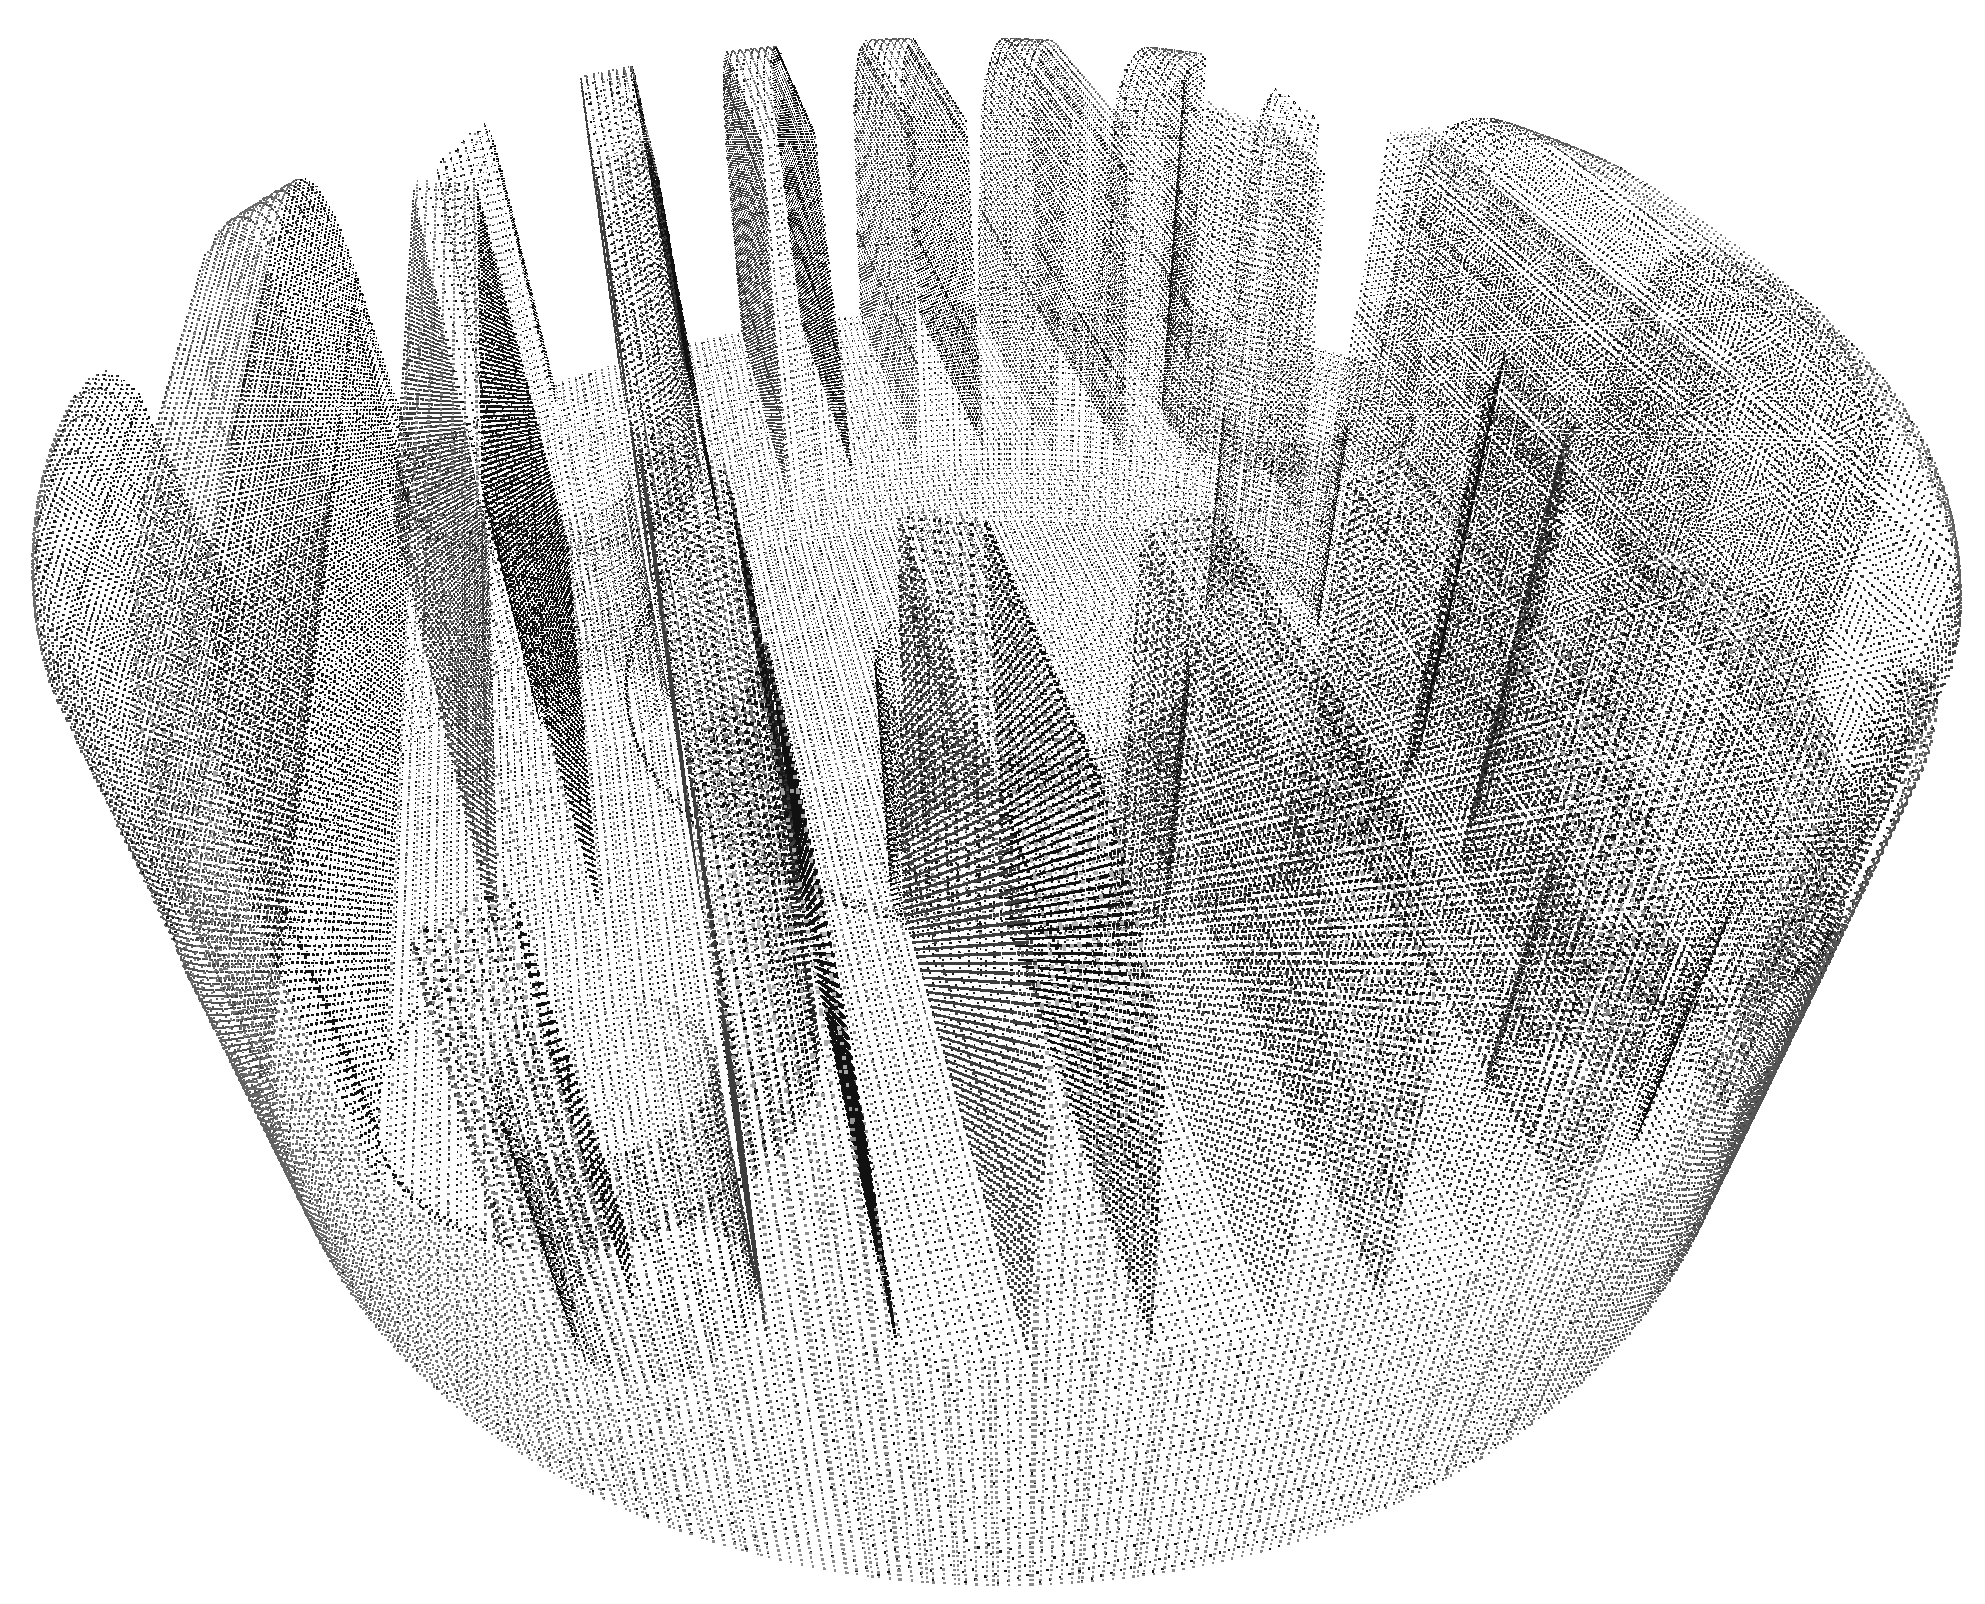
\includegraphics[width=\textwidth]{images/cylinder_head_point_cloud}
		\caption{cylinder\_head}
		\label{fig:cylinder_head_point_cloud_}
	\end{subfigure}
	\begin{subfigure}[t]{0.49\textwidth}
		\centering
		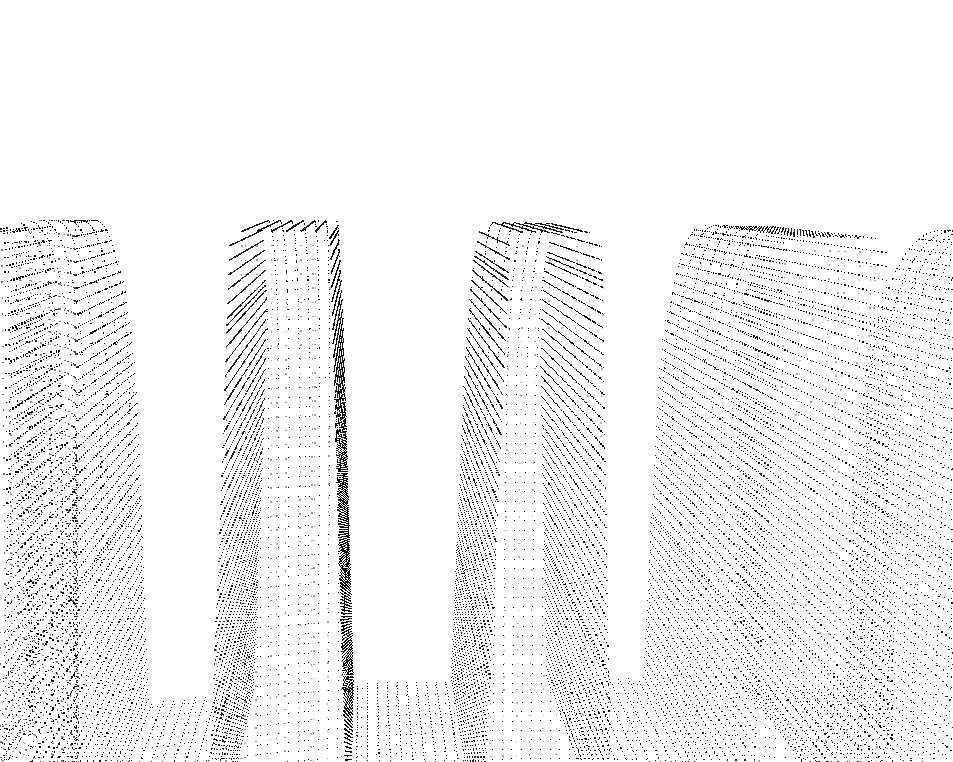
\includegraphics[width=\textwidth]{images/cylinder_head_point_cloud_fins}
		\caption{fins}
		\label{fig:cylinder_head_point_cloud_fins}
	\end{subfigure}
	\caption{
		Point cloud created by raycasting the cylinder\_head scene using three axis-aligned raycasts along the coordinate system's axes with a resolution of 200.
	}
	\label{fig:cylinder_head_point_cloud}
\end{figure}
%
Secondly, after the point cloud has been created, a surface reconstruction algorithm is run on it.

Regarding its quality, a point cloud sampled from the VML's regular grid using a uniform, axis-aligned raycast has a few properties:
\begin{itemize}
	\item
	All surface points, excluding numeric errors, are usually perfect samples, lying directly on the workpiece's surface.
	There is neither noise on the surface nor are there irrelevant inner or outer points.
	\item
	Each surface sample provides a perfect surface normal.
	\item
	The regularity of the raycaster guarantees a minimum and maximum density of the cloud, which may be derived from the distances between adjacent rays along each axis.
\end{itemize}

Despite these quality guarantees, a point cloud is still less rich in semantics when compared with a tri-dexel image.
The most prominent differences and commonalities are:
\begin{itemize}
	\item
	Point clouds only store surface information, whereas a tri-dexel image also holds volumetric information, \ie the dexel segments and point occupancy of the tri-dexel grid.
	\item
	Although a sufficient density is necessary, point clouds do not profit from the regular and uniform sampling.
	This property is fundamental for the tri-dexel approach, as it enables the construction of the regular tri-dexel grid and breaks down the problem of triangulation.
	\item
	The regularization of the tri-dexel cells provides a good way of detecting feature-rich regions which should be resampled with increased density.
	Such regions are harder to find within a point cloud, although local point distance and normal variance might give good hints.
	\item
	Although no regularization step is needed for small peculiarities of the cloud, it depends solely on the used reconstruction algorithm whether such small features are extracted or left unused.
	Regarding the tri-dexel approach presented in chapter \ref{ch:tri_dexel}, such behavior is well-defined by either regularizing, \ie dropping, or slicing a cell with small features.
	\item
	Regarding both data structures, features which are not discovered by the raycaster are not present in the built data structures.
	Subsequent algorithms have to implement some kind of feature reconstruction.
	\item
	Point clouds are simpler data structures and easier to exchange with other 3D software.
	\item
	Point clouds have a substantially smaller memory footprint than tri-dexel images.
\end{itemize}


\section{Implementation}
\label{sec:point_cloud_implementation}

Reusing the axis-aligned raycast from section \ref{sec:tri_dexel_raycast}, all reported surface intersections are just accumulated into a set of points.
Afterwards, any kind of surface reconstruction algorithm may used to proceed.

\subsection{Point cloud creation}
\label{sec:point_cloud_creation}

Algorithm \ref{alg:point_cloud_based} shows the basic routine used to obtain a point cloud and call a subsequent reconstruction algorithm.
%
\begin{algorithm}
	\centering
	\begin{algorithmic}[1]
		\Function{PointCloudBased}{$\var{grid}, \var{resolution}$}
			\State $\var{res} = \Call{UniformResolution}{\var{grid}.\var{aabb}, \var{resolution}}$
			\State $\var{cloud} = \varnothing$
			\State $\Call{AxisParallelRaycast}{\var{grid}, \var{grid}.\var{aabb}, \var{res},\hfill\break
				\hspace*{\dimexpr\algorithmicindent*2}(\var{\_}, \var{\_}, \var{\_}, \var{v}, \var{n}) \rightarrow \var{cloud}.\var{add}((\var{v}, \var{n}))}$
			\State \Return $\Call{ReconstructFromPointCloud}{\var{cloud}}$
		\EndFunction
	\end{algorithmic}
	\caption{
		Abstract workflow of the surface reconstruction using an arbitrary point cloud reconstruction algorithm \textproc{ReconstructFromPointCloud}.
	}
	\label{alg:point_cloud_based}
\end{algorithm}
%
Using the \textproc{UniformResolution} function, the algorithm starts off by computing an appropriate raycasting resolution \var{res} for all three axes, based on the \var{resolution} parameter passed by the user.
This step is also done before the tri-dexel raycast, but with an increased bounding box, \cf algorithm \ref{alg:tri_dexel}.
For the details of \textproc{UniformResolution} \cf section \ref{sec:tri_dexel_implementation}.
Afterwards, an empty set of points, \var{cloud}, is created, which will accumulate all surface points emitted by the raycaster.
Afterwards, the raycast is launched with the calculated resolution and the grid's bounding box.
The closure passed to the raycasting subroutine \textproc{AxisParallelRaycast} is called at every surface hit with a list of arguments.
From these arguments only the last two, the intersection point \var{v} and the corresponding surface normal \var{n}, are relevant.
These two are added as tuple to the current point cloud \var{cloud}.
Mind that the closure is invoked concurrently, requiring $\var{cloud}.\var{add}$ to be thread-safe.
After the raycast has finished, a point cloud based surface reconstruction algorithm is run, indicated by the call to \textproc{ReconstructFromPointCloud}.

\subsection{Surface reconstruction}
\label{sec:point_cloud_reconstruction}

Two examples of algorithms for surface reconstruction from point clouds are given in the following:

\begin{description}
	\begin{figure}
		\centering
		\begin{subfigure}[b]{0.30\textwidth}
			\centering
			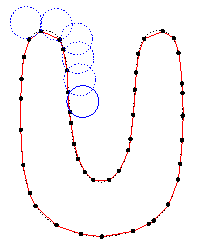
\includegraphics[width=\textwidth]{bpa_principle_1}
			\caption{
				Pivoting
			}
			\label{fig:bpa_principle_1}
		\end{subfigure}
		\begin{subfigure}[b]{0.30\textwidth}
			\centering
			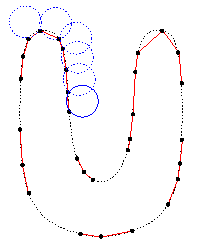
\includegraphics[width=\textwidth]{bpa_principle_2}
			\caption{
				Hole creation
			}
			\label{fig:bpa_principle_2}
		\end{subfigure}
		\begin{subfigure}[b]{0.30\textwidth}
			\centering
			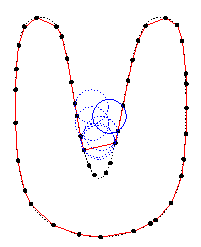
\includegraphics[width=\textwidth]{bpa_principle_3}
			\caption{
				Lost features
			}
			\label{fig:bpa_principle_3}
		\end{subfigure}
		\caption{
			Principle of the BPA surface reconstruction approach \cite{bpa}.
		}
		\label{fig:bpa_principle}
	\end{figure}

	\item[Ball pivoting algorithm] \hfill \\
	The ball pivoting algorithm (BPA) is a region growing algorithm, \cf figure \ref{fig:bpa_principle}.
	As the name suggests, it places a ball, \ie sphere, at the outside of the point cloud, touching three points, creating a seed triangle.
	From this seed triangle, the ball is pivoted over each edge of the triangle until it touches another point, creating a new triangle with new edges to roll over.
	If no point is found during pivoting, the edge is left as a boundary.
	The front of edges is rolled over repeatedly until no more edges are available.
	If all pivots where successful, a closed, manifold and oriented mesh has been created.
	The BPA requires a user supplied ball size, which steers the capability of rolling into finer features and the danger of creating holes or falling into the point cloud.
	If the point density is too low or the ball is too small, holes are created, \cf figure \ref{fig:bpa_principle_2}.
	If concave features are too small or the ball is too large, features may be lost, \cf figure \ref{fig:bpa_principle_3}.

	A highly tuned version of the BPA with elements of the G2S algorithm is already utilized by the VML for its swept volume computation \cite{bpa_vml}.
	A further implementation of the BPA is available in CGAL \cite{cgal_bpa}.
	MeshLab also offers a BPA version, parameterizable via its GUI.
	The BPA will be the main example for a point cloud surface reconstruction algorithm throughout this chapter, especially the results section \ref{sec:point_cloud_results}.

%	\begin{figure}
%		\centering
%		\begin{subfigure}[b]{0.30\textwidth}
%			\centering
%			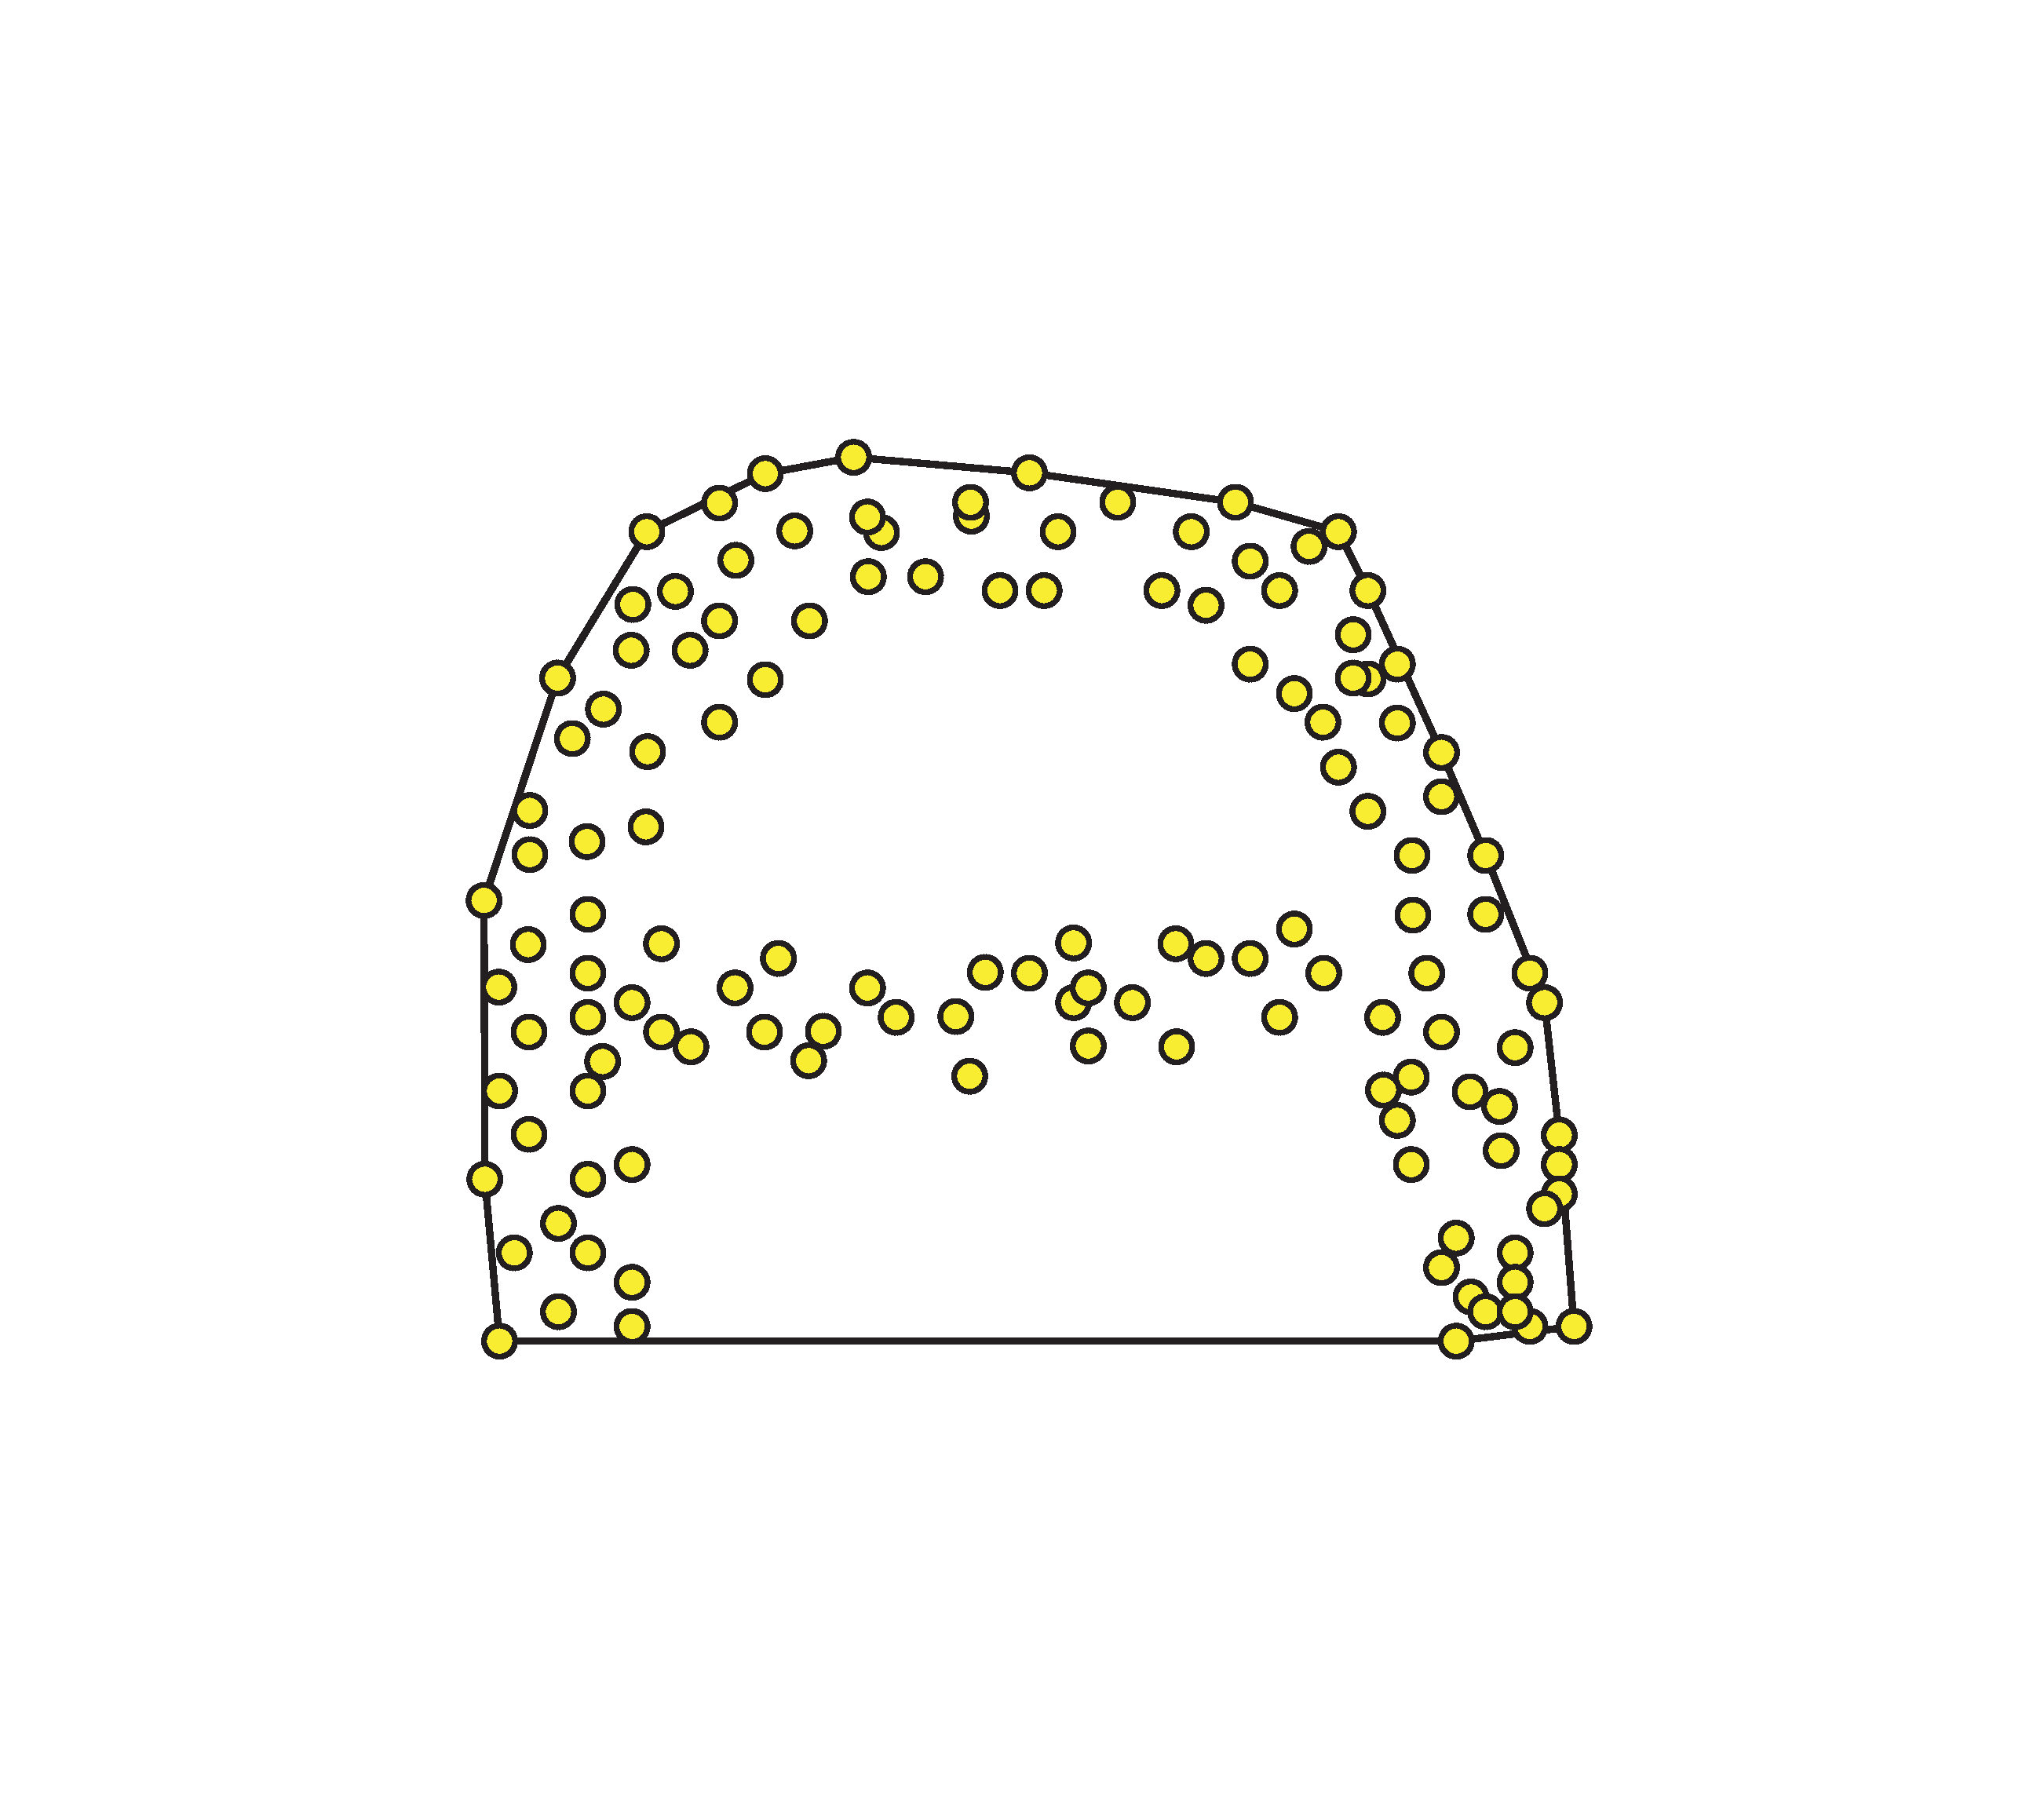
\includegraphics[width=\textwidth]{alpha_shapes_convex_hull}
%			\caption{
%				$\alpha = \infty$
%			}
%			\label{fig:alpha_shapes_convex_hull}
%		\end{subfigure}
%		\begin{subfigure}[b]{0.30\textwidth}
%			\centering
%			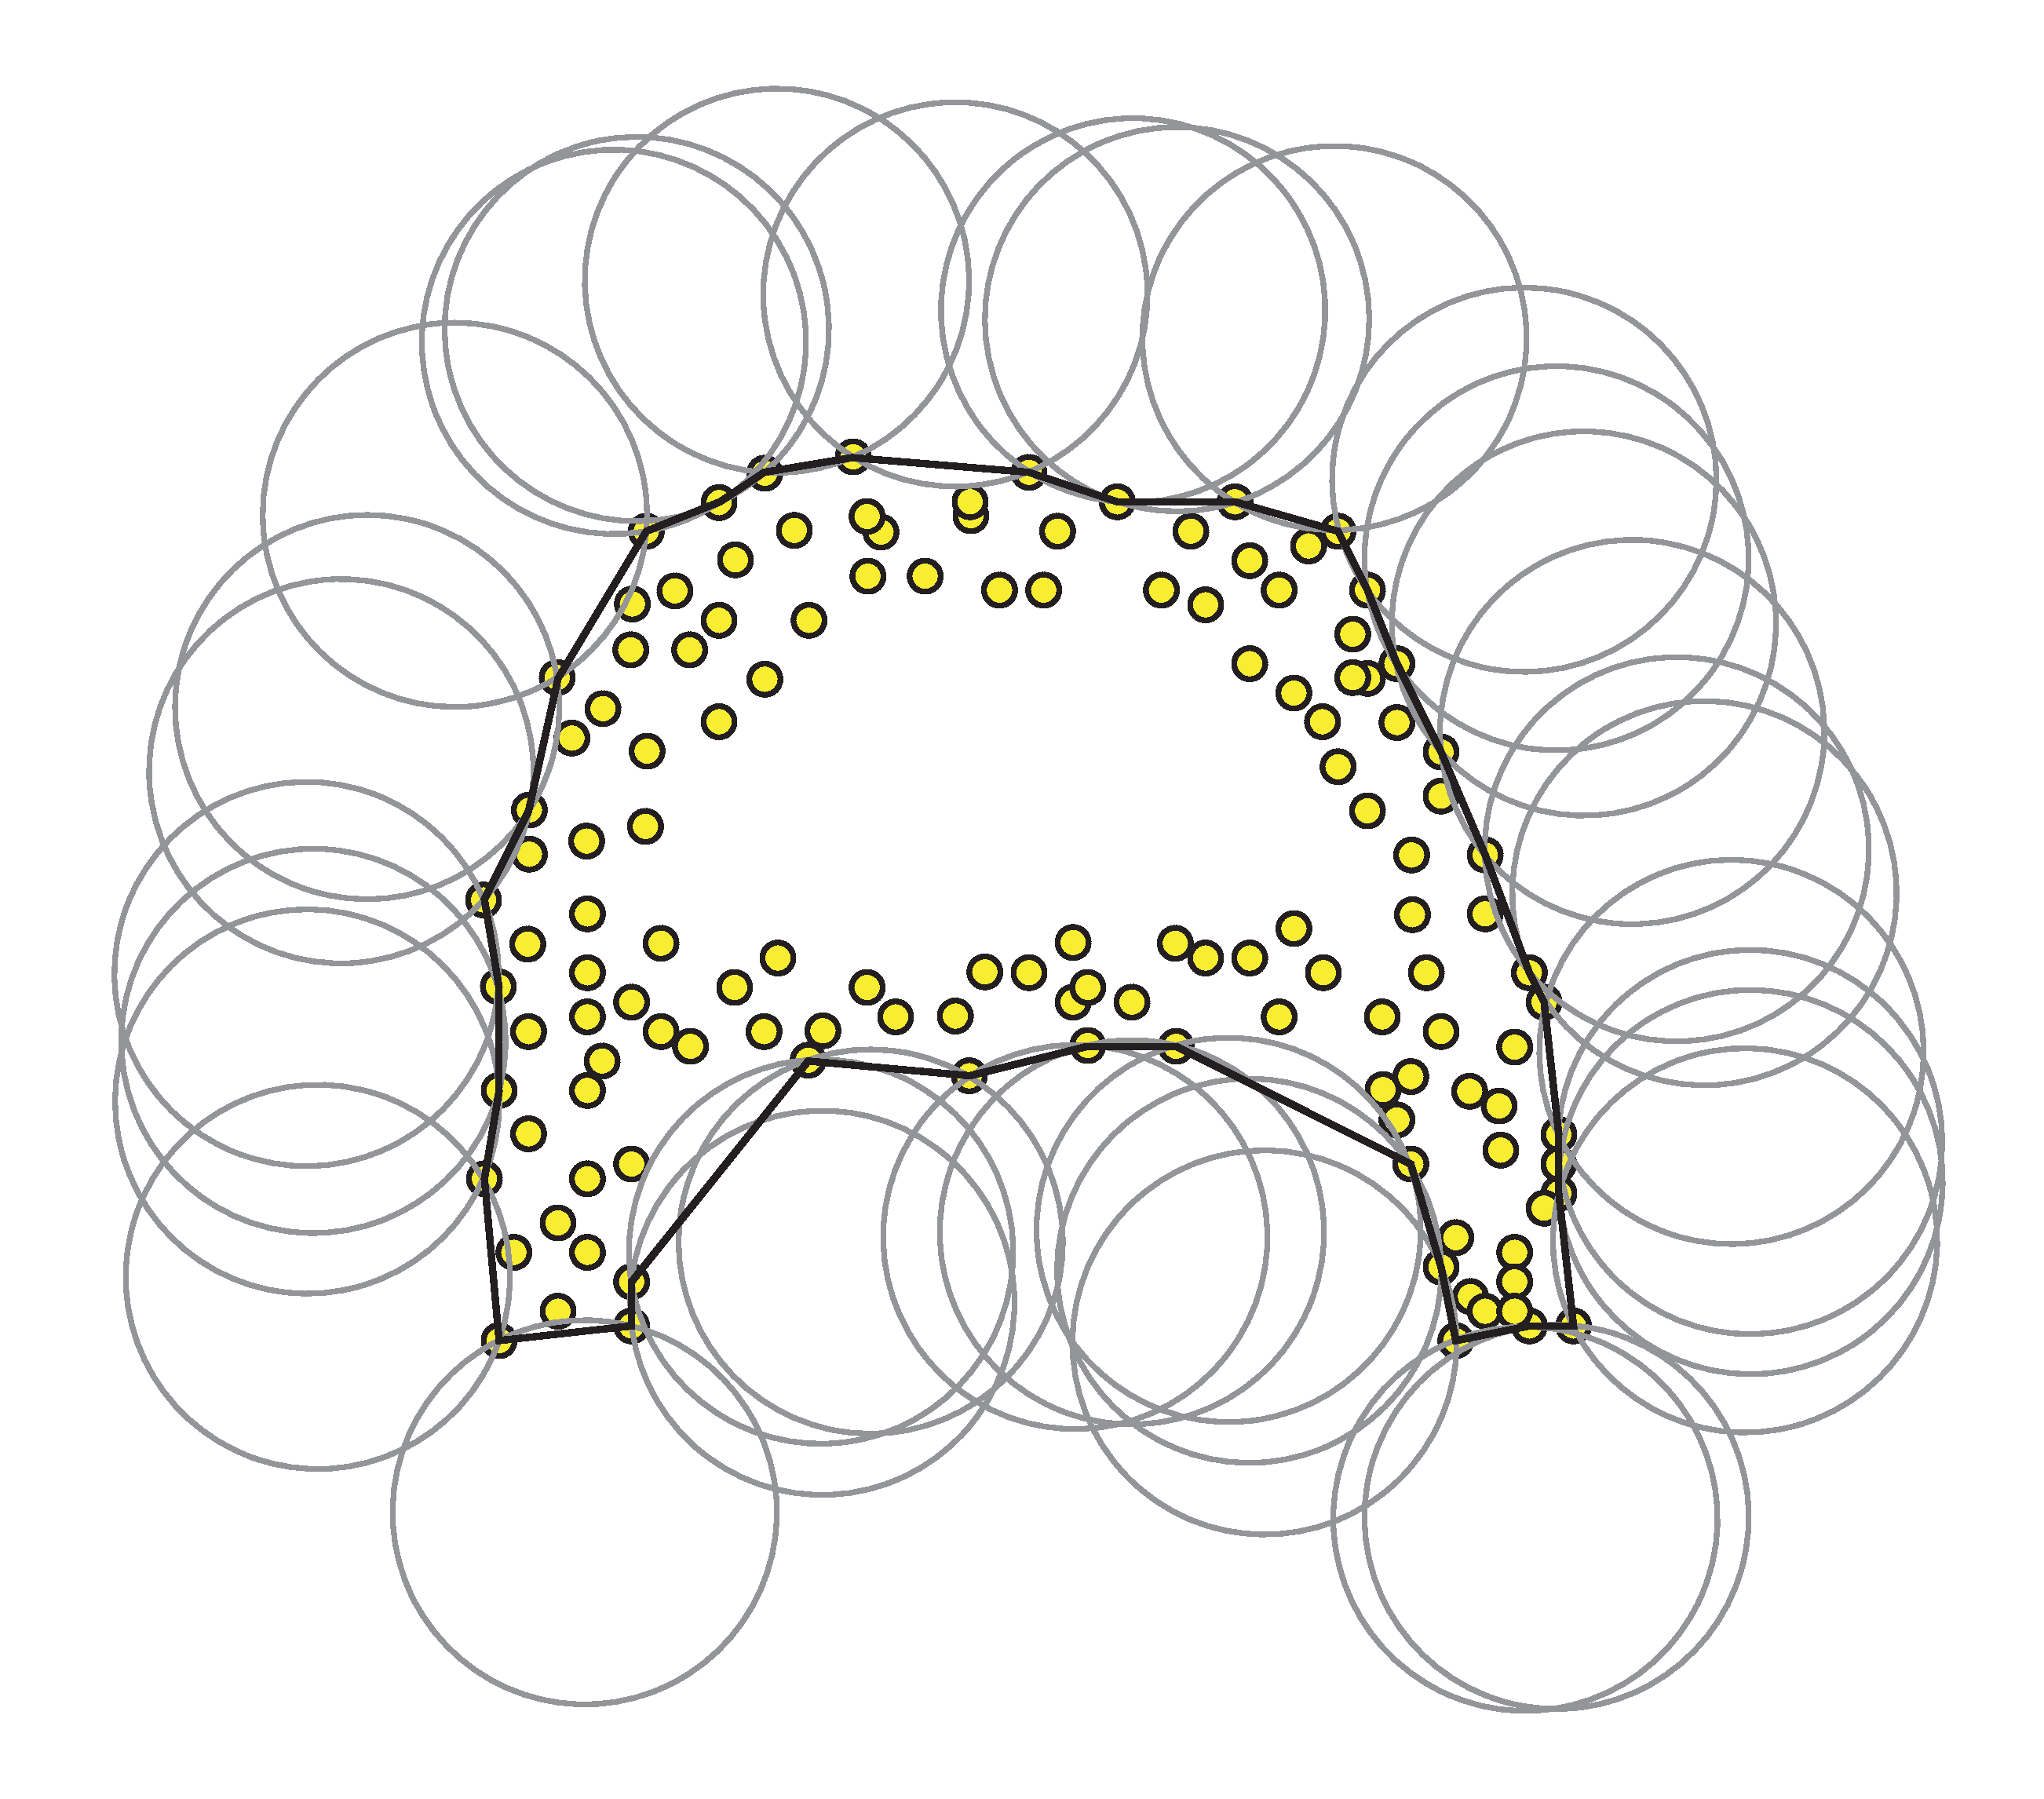
\includegraphics[width=\textwidth]{alpha_shapes_big_alpha}
%			\caption{
%				Big $\alpha$
%			}
%			\label{fig:alpha_shapes_big_alpha}
%		\end{subfigure}
%		\begin{subfigure}[b]{0.30\textwidth}
%			\centering
%			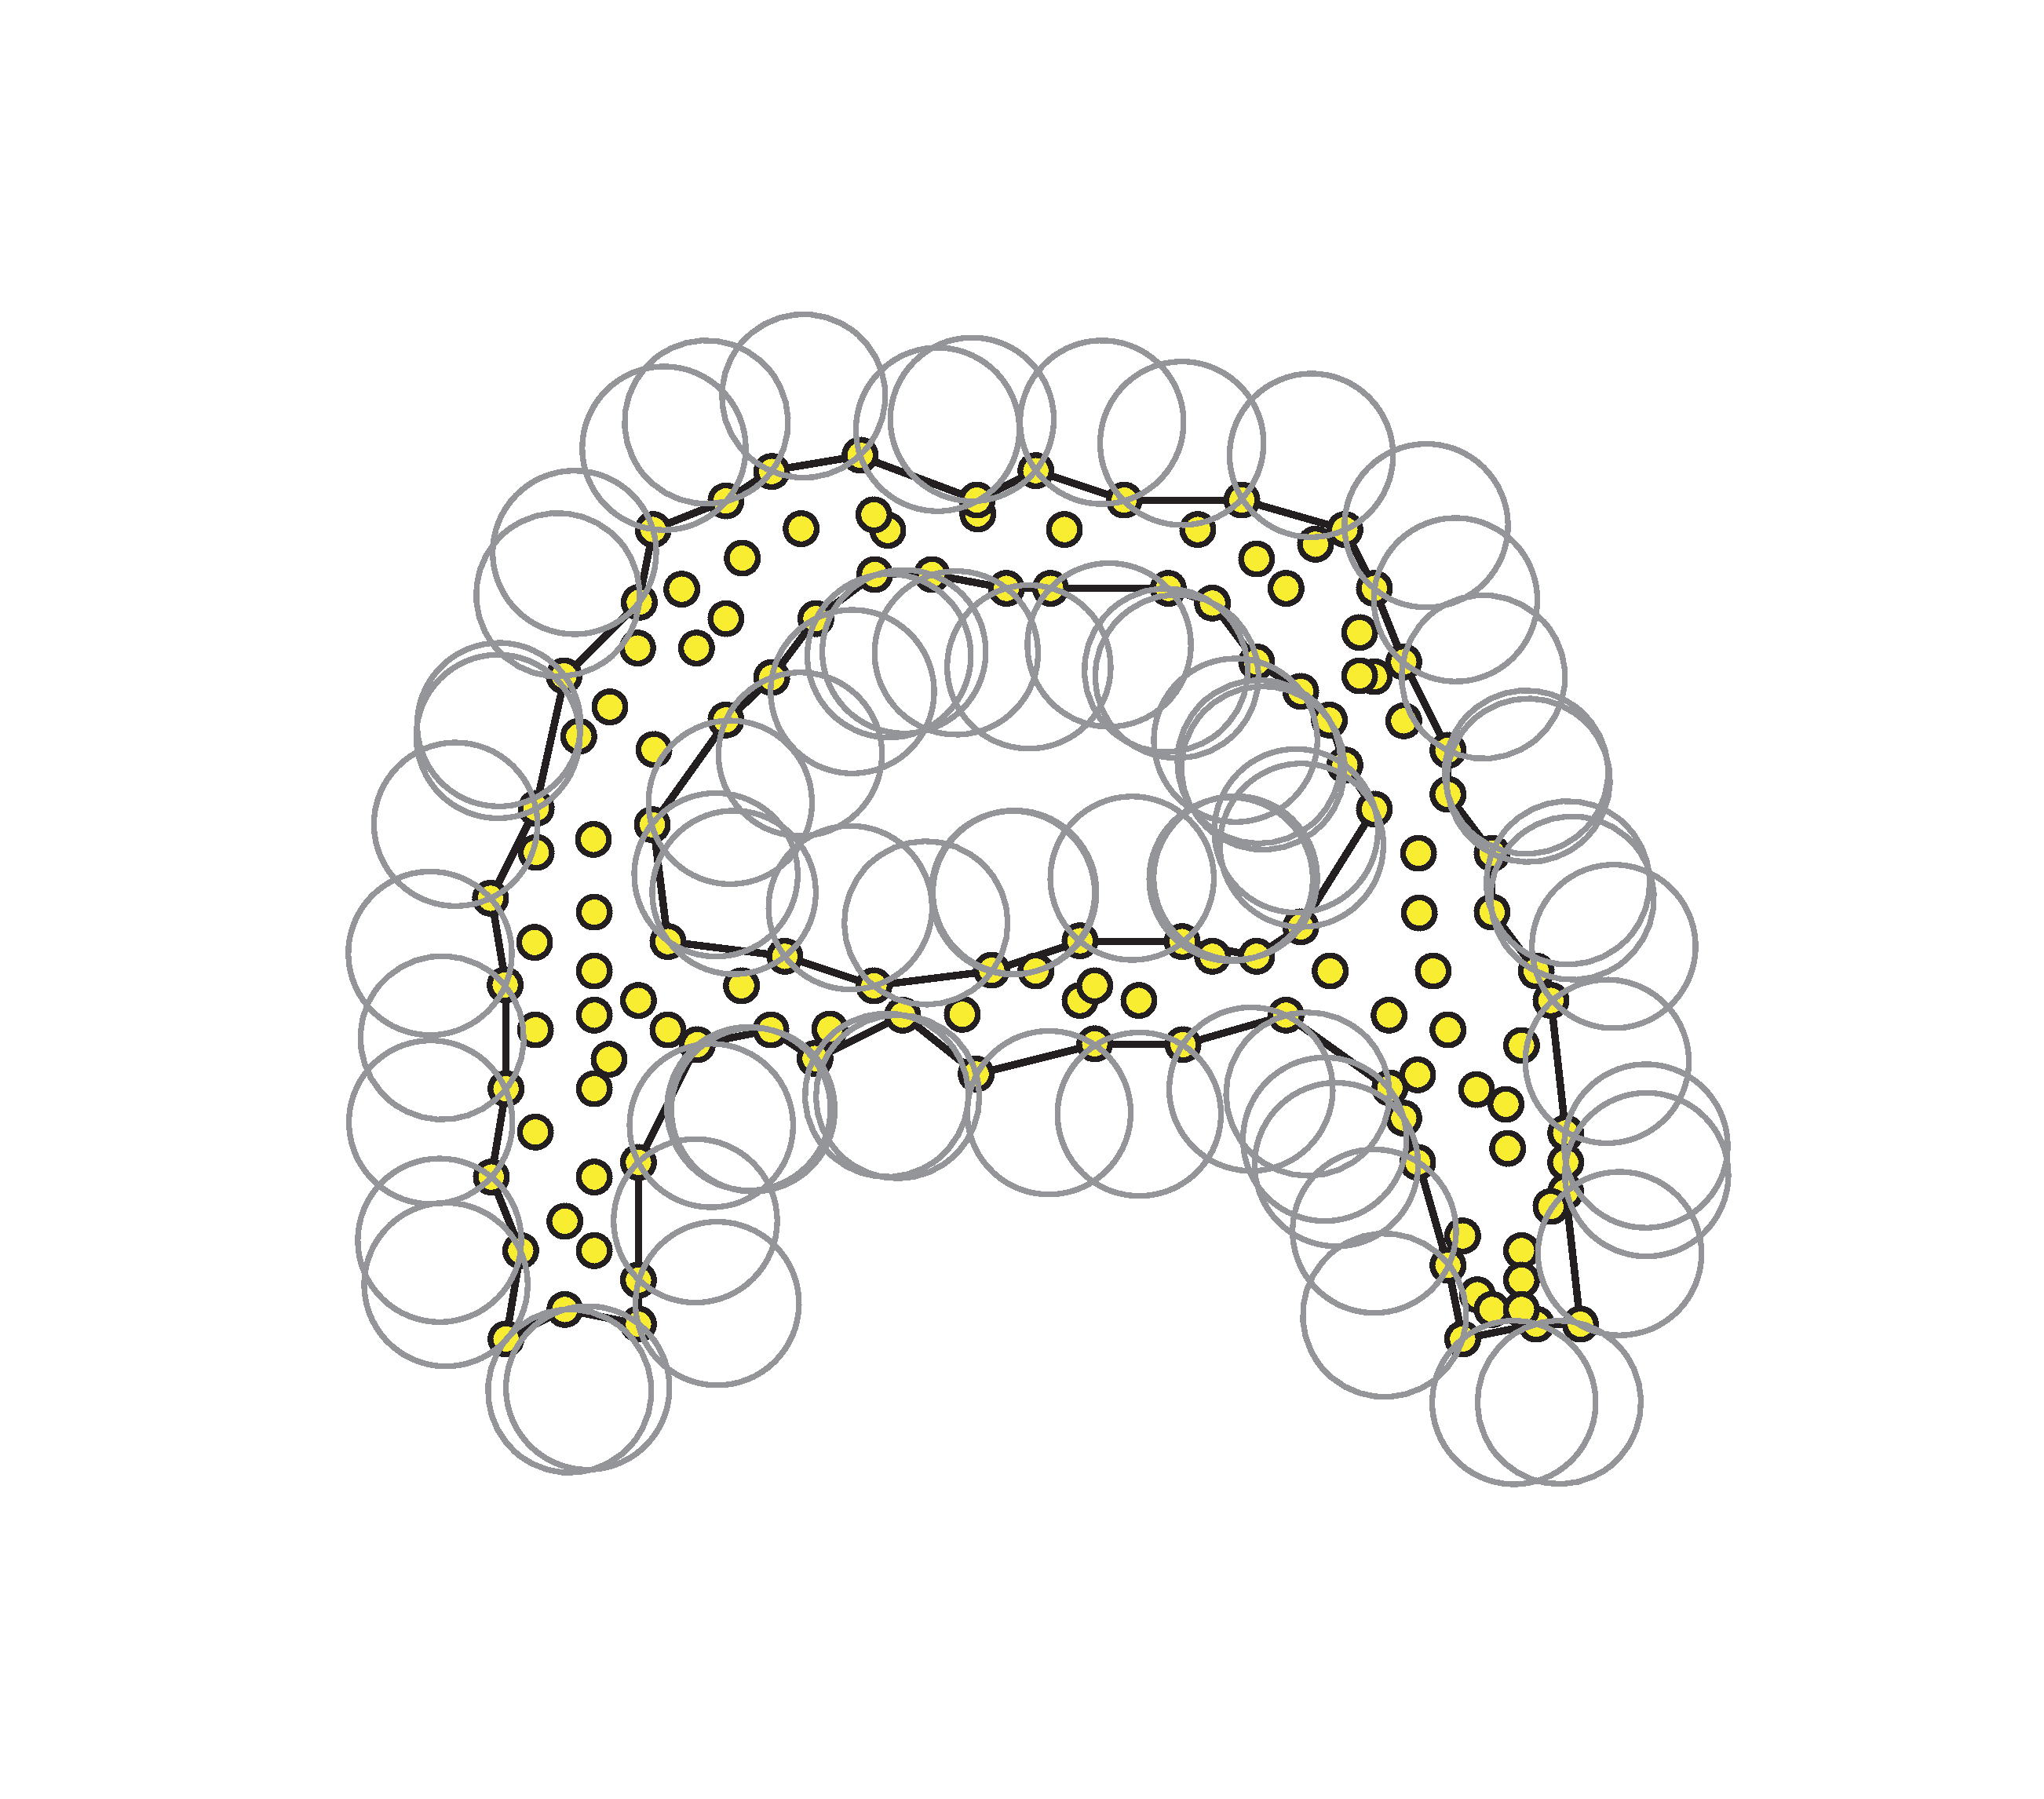
\includegraphics[width=\textwidth]{alpha_shapes_small_alpha}
%			\caption{
%				Small $\alpha$
%			}
%			\label{fig:alpha_shapes_small_alpha}
%		\end{subfigure}
%		\caption{
%			Principle of the alpha shapes surface reconstruction approach.
%			Based on \cite{alpha_shapes_images}.
%		}
%		\label{fig:alpha_shapes_principle}
%	\end{figure}
%
%	\item[$\alpha$-shape] \hfill \\
%	The $\alpha$-shape was one of the first tries to define a \enquote{shape} for a set of finite points \cite{alpha_shape}.
%	The $\alpha$-shape of a 3-dimensional point cloud is a set of triangles, where each triangle has at least one empty circumsphere with radius $\alpha$, \cf figure \ref{fig:alpha_shapes_principle}
%	It is quite similar to the BPA, but formulated statically, as no ball is rolled along the surface.
%	The $\alpha$-shape therefore also contains triangles within the point cloud, which would not be discovered by the BPA if the ball never rolls \enquote{inside} the point cloud, \ie sufficient density is given.
%	If $\alpha$ becomes $\infty$, the $\alpha$-shape becomes the convex hull of the point cloud, \cf figure \ref{fig:alpha_shapes_convex_hull}.
%	The magnitude of $\alpha$ determines
%	The empty circumsphere criterion further guarantees the triangulation to be Delaunay, \ie the $\alpha$-shape is a subset of the 3-dimensional Delaunay triangulation.
%	An implementation of an $\alpha$-shape constructing algorithm is found in \eg the CGAL \cite{cgal_3d_alpha_shapes}, VTK \cite{vtk}, QHull \cite{qhull} or PCL \cite{pcl} library.
%	MeshLab provides user-friendly access the QHull version of the algorithm via a GUI.

	\begin{figure}
		\centering
		\begin{subfigure}[b]{0.24\textwidth}
			\centering
			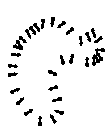
\includegraphics[width=\textwidth]{poisson_oriented_points}
			\captionsetup{justification=centering}
			\caption{
				oriented points\\
				$V$
			}
			\label{fig:poisson_oriented_points}
		\end{subfigure}
		\begin{subfigure}[b]{0.24\textwidth}
			\centering
			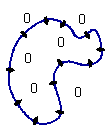
\includegraphics[width=\textwidth]{poisson_gradient_function}
			\captionsetup{justification=centering}
			\caption{
				indicator gradient\\
				$\nabla\chi$
			}
			\label{fig:poisson_gradient_function}
		\end{subfigure}
		\begin{subfigure}[b]{0.24\textwidth}
			\centering
			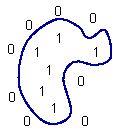
\includegraphics[width=\textwidth]{poisson_indicator_function}
			\captionsetup{justification=centering}
			\caption{
				indicator\\
				$\chi$
			}
			\label{fig:poisson_indicator_function}
		\end{subfigure}
		\begin{subfigure}[b]{0.24\textwidth}
			\centering
			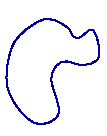
\includegraphics[width=\textwidth]{poisson_surface}
			\captionsetup{justification=centering}
			\caption{
				surface\\
				~
			}
			\label{fig:poisson_surface}
		\end{subfigure}
		\caption{
			Principle of the Poisson surface reconstruction approach \cite{poisson}.
		}
		\label{fig:poisson_principle}
	\end{figure}

	\item[Poisson] \hfill \\
	Poisson surface reconstruction is based on implicit functions \cite{poisson}, \cf figure \ref{fig:poisson_principle}.
	The goal is to compute a so-called indicator function $\chi$, which yields 1 for positions inside the workpiece and 0 for positions outside, \cf figure \ref{fig:poisson_indicator_function}
	When moving into the workpiece from outside, the values of $\chi$ change from 0 to 1 around the surface.
	The indicator function $\chi$, specifically its gradient $\nabla\chi$, \cf figure \ref{fig:poisson_gradient_function}, is strongly related to the normals of the input point set, a vector field $V$, \cf figure \ref{fig:poisson_oriented_points}.
	Therefore, the problem becomes finding a function $\chi$ whose gradient $\nabla\chi$ best approximates $V$, the normals of the point cloud, \ie $\min_\chi |\nabla\chi - V|$.
	This problem is then transformed into a standard Poisson problem, further details are given in the corresponding paper \cite{poisson}.
	For the computation of these functions, the problem space is partitioned using an octree, whose depth provides the main variable to balance memory/computational demands and reconstruction quality.
	The reconstruction of a surface is finally done by extracting an isosurface of $\chi$.

	Implementations of Poisson surface reconstruction are found in \eg the CGAL \cite{cgal_poisson}, VTK \cite{vtk_poisson} and PCL \cite{pcl} library.
	MeshLab also integrates a Poisson implementation into its GUI.
\end{description}


\section{Results}
\label{sec:point_cloud_results}

The point cloud creation and the subsequent reconstruction using the BPA discussed in \ref{sec:point_cloud_reconstruction} have been benchmarked for the test scenes described in section \ref{sec:test_scenes}.
Analogously to the tri-dexel benchmarks, the resolutions 50, 100, 200 and 400 have been used for the raycaster creating the point clouds.
Table \ref{tbl:point_cloud_results} contains the runtime and output size of the created point clouds.
%
\begin{table}
	\begin{tabular}{l|rr|rr|rr|rr}
		resolution     & \multicolumn{2}{c}{50} & \multicolumn{2}{c}{100} & \multicolumn{2}{c}{200} & \multicolumn{2}{c}{400} \\
		scene          & p\sub{out} & time & p\sub{out} & time & p\sub{out} & time & p\sub{out} & time \\
		\midrule
		cube2          & \SI{14}{\kilo\nothing} & \SI{  3}{\milli\second} & \SI{56}{\kilo\nothing} & \SI{ 12}{\milli\second} & \SI{226}{\kilo\nothing} & \SI{  47}{\milli\second} & \SI{907}{\kilo\nothing} & \SI{ 187}{\milli\second} \\
		cylinders\_d   & \SI{ 7}{\kilo\nothing} & \SI{  5}{\milli\second} & \SI{27}{\kilo\nothing} & \SI{ 17}{\milli\second} & \SI{108}{\kilo\nothing} & \SI{  63}{\milli\second} & \SI{436}{\kilo\nothing} & \SI{ 247}{\milli\second} \\
		cylinders      & \SI{ 7}{\kilo\nothing} & \SI{  3}{\milli\second} & \SI{26}{\kilo\nothing} & \SI{ 11}{\milli\second} & \SI{107}{\kilo\nothing} & \SI{  41}{\milli\second} & \SI{433}{\kilo\nothing} & \SI{ 161}{\milli\second} \\
		cylinder\_head & \SI{15}{\kilo\nothing} & \SI{  7}{\milli\second} & \SI{60}{\kilo\nothing} & \SI{ 23}{\milli\second} & \SI{242}{\kilo\nothing} & \SI{  86}{\milli\second} & \SI{976}{\kilo\nothing} & \SI{ 335}{\milli\second} \\
		impeller       & \SI{11}{\kilo\nothing} & \SI{ 99}{\milli\second} & \SI{46}{\kilo\nothing} & \SI{353}{\milli\second} & \SI{184}{\kilo\nothing} & \SI{1118}{\milli\second} & \SI{744}{\kilo\nothing} & \SI{3813}{\milli\second} \\
		impeller\_2    & \SI{ 9}{\kilo\nothing} & \SI{ 54}{\milli\second} & \SI{38}{\kilo\nothing} & \SI{193}{\milli\second} & \SI{155}{\kilo\nothing} & \SI{ 600}{\milli\second} & \SI{625}{\kilo\nothing} & \SI{2037}{\milli\second} \\
		turbine        & \SI{ 7}{\kilo\nothing} & \SI{165}{\milli\second} & \SI{31}{\kilo\nothing} & \SI{650}{\milli\second} & \SI{132}{\kilo\nothing} & \SI{2509}{\milli\second} & \SI{532}{\kilo\nothing} & \SI{9610}{\milli\second} \\
	\end{tabular}
	\caption{
		Test results for the point cloud creation.
		Benchmarks were run on a machine utilizing an Intel Core i7-3770 at \SI{3.4}{\giga\hertz} with \SI{16}{\gibi\byte} RAM.
		Runtime is averaged over 10 runs.
	}
	\label{tbl:point_cloud_results}
\end{table}
%
Three trends, similarly to the results of the tri-dexel reconstruction in table \ref{tbl:tri_dexel_results}, are also observable here.
Firstly, the number of created points p\sub{out} for a given resolution is again similar for all scenes.
Secondly, p\sub{out} increases quadratically with the resolution.
Thirdly, also the runtime increases quadratically with the resolution.
The reasons is the asymptotic complexity of $\mathcal{O}(n^2)$ of the raycaster, which is discussed in more detail in section \ref{sec:tri_dexel_results}.
Furthermore, the dependency of the runtime on the scene's complexity as well as parallelization, CPU and memory consumption is also discussed there.

Concerning subsequent surface reconstruction algorithms, table \ref{tbl:bpa_results} contains the mesh sizes and timings for the VML's BPA implementation.
The ball's radius is derived from the raycasting resolution and set to 1.5 times the diameter of a cell of the sampling grid created by 3 axis aligned raycasts.
%
\begin{table}
	\centering
	\begin{tabular}{l|rrr|rrr}
		resolution     & \multicolumn{3}{c}{50} & \multicolumn{3}{c}{100} \\
		scene          & p\sub{in} & t\sub{out} & time & p\sub{in} & t\sub{out} & time \\
		\midrule
		cube2          & \SI{14}{\kilo\nothing}& \SI{27}{\kilo\nothing} & \SI{53}{\milli\second} & \SI{56}{\kilo\nothing} & \SI{111}{\kilo\nothing} & \SI{222}{\milli\second} \\
		cylinders\_d   & \SI{ 7}{\kilo\nothing}& \SI{13}{\kilo\nothing} & \SI{22}{\milli\second} & \SI{27}{\kilo\nothing} & \SI{ 53}{\kilo\nothing} & \SI{ 95}{\milli\second} \\
		cylinders      & \SI{ 7}{\kilo\nothing}& \SI{13}{\kilo\nothing} & \SI{22}{\milli\second} & \SI{26}{\kilo\nothing} & \SI{ 53}{\kilo\nothing} & \SI{ 94}{\milli\second} \\
		cylinder\_head & \SI{15}{\kilo\nothing}& \SI{27}{\kilo\nothing} & \SI{60}{\milli\second} & \SI{60}{\kilo\nothing} & \SI{110}{\kilo\nothing} & \SI{223}{\milli\second} \\
		impeller       & \SI{11}{\kilo\nothing}& \SI{20}{\kilo\nothing} & \SI{48}{\milli\second} & \SI{46}{\kilo\nothing} & \SI{ 91}{\kilo\nothing} & \SI{200}{\milli\second} \\
		impeller\_2    & \SI{ 9}{\kilo\nothing}& \SI{17}{\kilo\nothing} & \SI{36}{\milli\second} & \SI{38}{\kilo\nothing} & \SI{ 76}{\kilo\nothing} & \SI{161}{\milli\second} \\
		turbine        & \SI{ 7}{\kilo\nothing}& \SI{ 9}{\kilo\nothing} & \SI{20}{\milli\second} & \SI{31}{\kilo\nothing} & \SI{ 53}{\kilo\nothing} & \SI{142}{\milli\second} \\

		\multicolumn{1}{l}{\bigskip} \\

		resolution     & \multicolumn{3}{c}{200} & \multicolumn{3}{c}{400} \\
		scene          & p\sub{in} & t\sub{out} & time & p\sub{in} & t\sub{out} & time \\
		\midrule
		cube2          & \SI{226}{\kilo\nothing}& \SI{449}{\kilo\nothing} & \SI{1022}{\milli\second} & \SI{907}{\kilo\nothing}& \SI{1807}{\kilo\nothing} & \SI{5106}{\milli\second} \\
		cylinders\_d   & \SI{108}{\kilo\nothing}& \SI{217}{\kilo\nothing} & \SI{ 442}{\milli\second} & \SI{436}{\kilo\nothing}& \SI{ 871}{\kilo\nothing} & \SI{1999}{\milli\second} \\
		cylinders      & \SI{107}{\kilo\nothing}& \SI{215}{\kilo\nothing} & \SI{ 421}{\milli\second} & \SI{433}{\kilo\nothing}& \SI{ 865}{\kilo\nothing} & \SI{1902}{\milli\second} \\
		cylinder\_head & \SI{242}{\kilo\nothing}& \SI{454}{\kilo\nothing} & \SI{ 946}{\milli\second} & \SI{976}{\kilo\nothing}& \SI{1850}{\kilo\nothing} & \SI{4263}{\milli\second} \\
		impeller       & \SI{184}{\kilo\nothing}& \SI{368}{\kilo\nothing} & \SI{ 859}{\milli\second} & \SI{744}{\kilo\nothing}& \SI{1485}{\kilo\nothing} & \SI{3710}{\milli\second} \\
		impeller\_2    & \SI{155}{\kilo\nothing}& \SI{309}{\kilo\nothing} & \SI{ 695}{\milli\second} & \SI{625}{\kilo\nothing}& \SI{1248}{\kilo\nothing} & \SI{3135}{\milli\second} \\
		turbine        & \SI{132}{\kilo\nothing}& \SI{246}{\kilo\nothing} & \SI{ 613}{\milli\second} & \SI{532}{\kilo\nothing}& \SI{1049}{\kilo\nothing} & \SI{2222}{\milli\second} \\
	\end{tabular}
	\caption{
		Test results surface reconstruction using the VML's internal BPA implementation excluding the time required to generate the point cloud, \cf table \ref{tbl:point_cloud_results}.
		Benchmarks were run on a machine utilizing an Intel Core i7-3770 at \SI{3.4}{\giga\hertz} with \SI{16}{\gibi\byte} RAM.
		Runtime is averaged over 10 runs.
	}
	\label{tbl:bpa_results}
\end{table}
%
Compared with the tri-dexel results in table \ref{tbl:tri_dexel_results}, the BPA outputs less than a half as much triangles.
This is due to the additional feature reconstruction and triangle fans created inside each cell by the tri-dexel approach.
As the BPA only operates on the vertices of the point cloud, it cannot create any further vertices.

Another consequence of this behavior is a correlation of the number of input points, \cf table \ref{tbl:point_cloud_results}, and the number of outputted triangles, \cf table \ref{tbl:bpa_results}.
For each point of the input roughly two triangles are created.
This ratio is smaller at lower resolutions as more features/points are skipped by the ball's size, but, with increasing density, almost all points are used by the BPA and this ratio approaches two.
An explanation for this ratio is given in figure \ref{fig:bpa_point_triangle_ratio}.
%
\begin{figure}
	\centering
	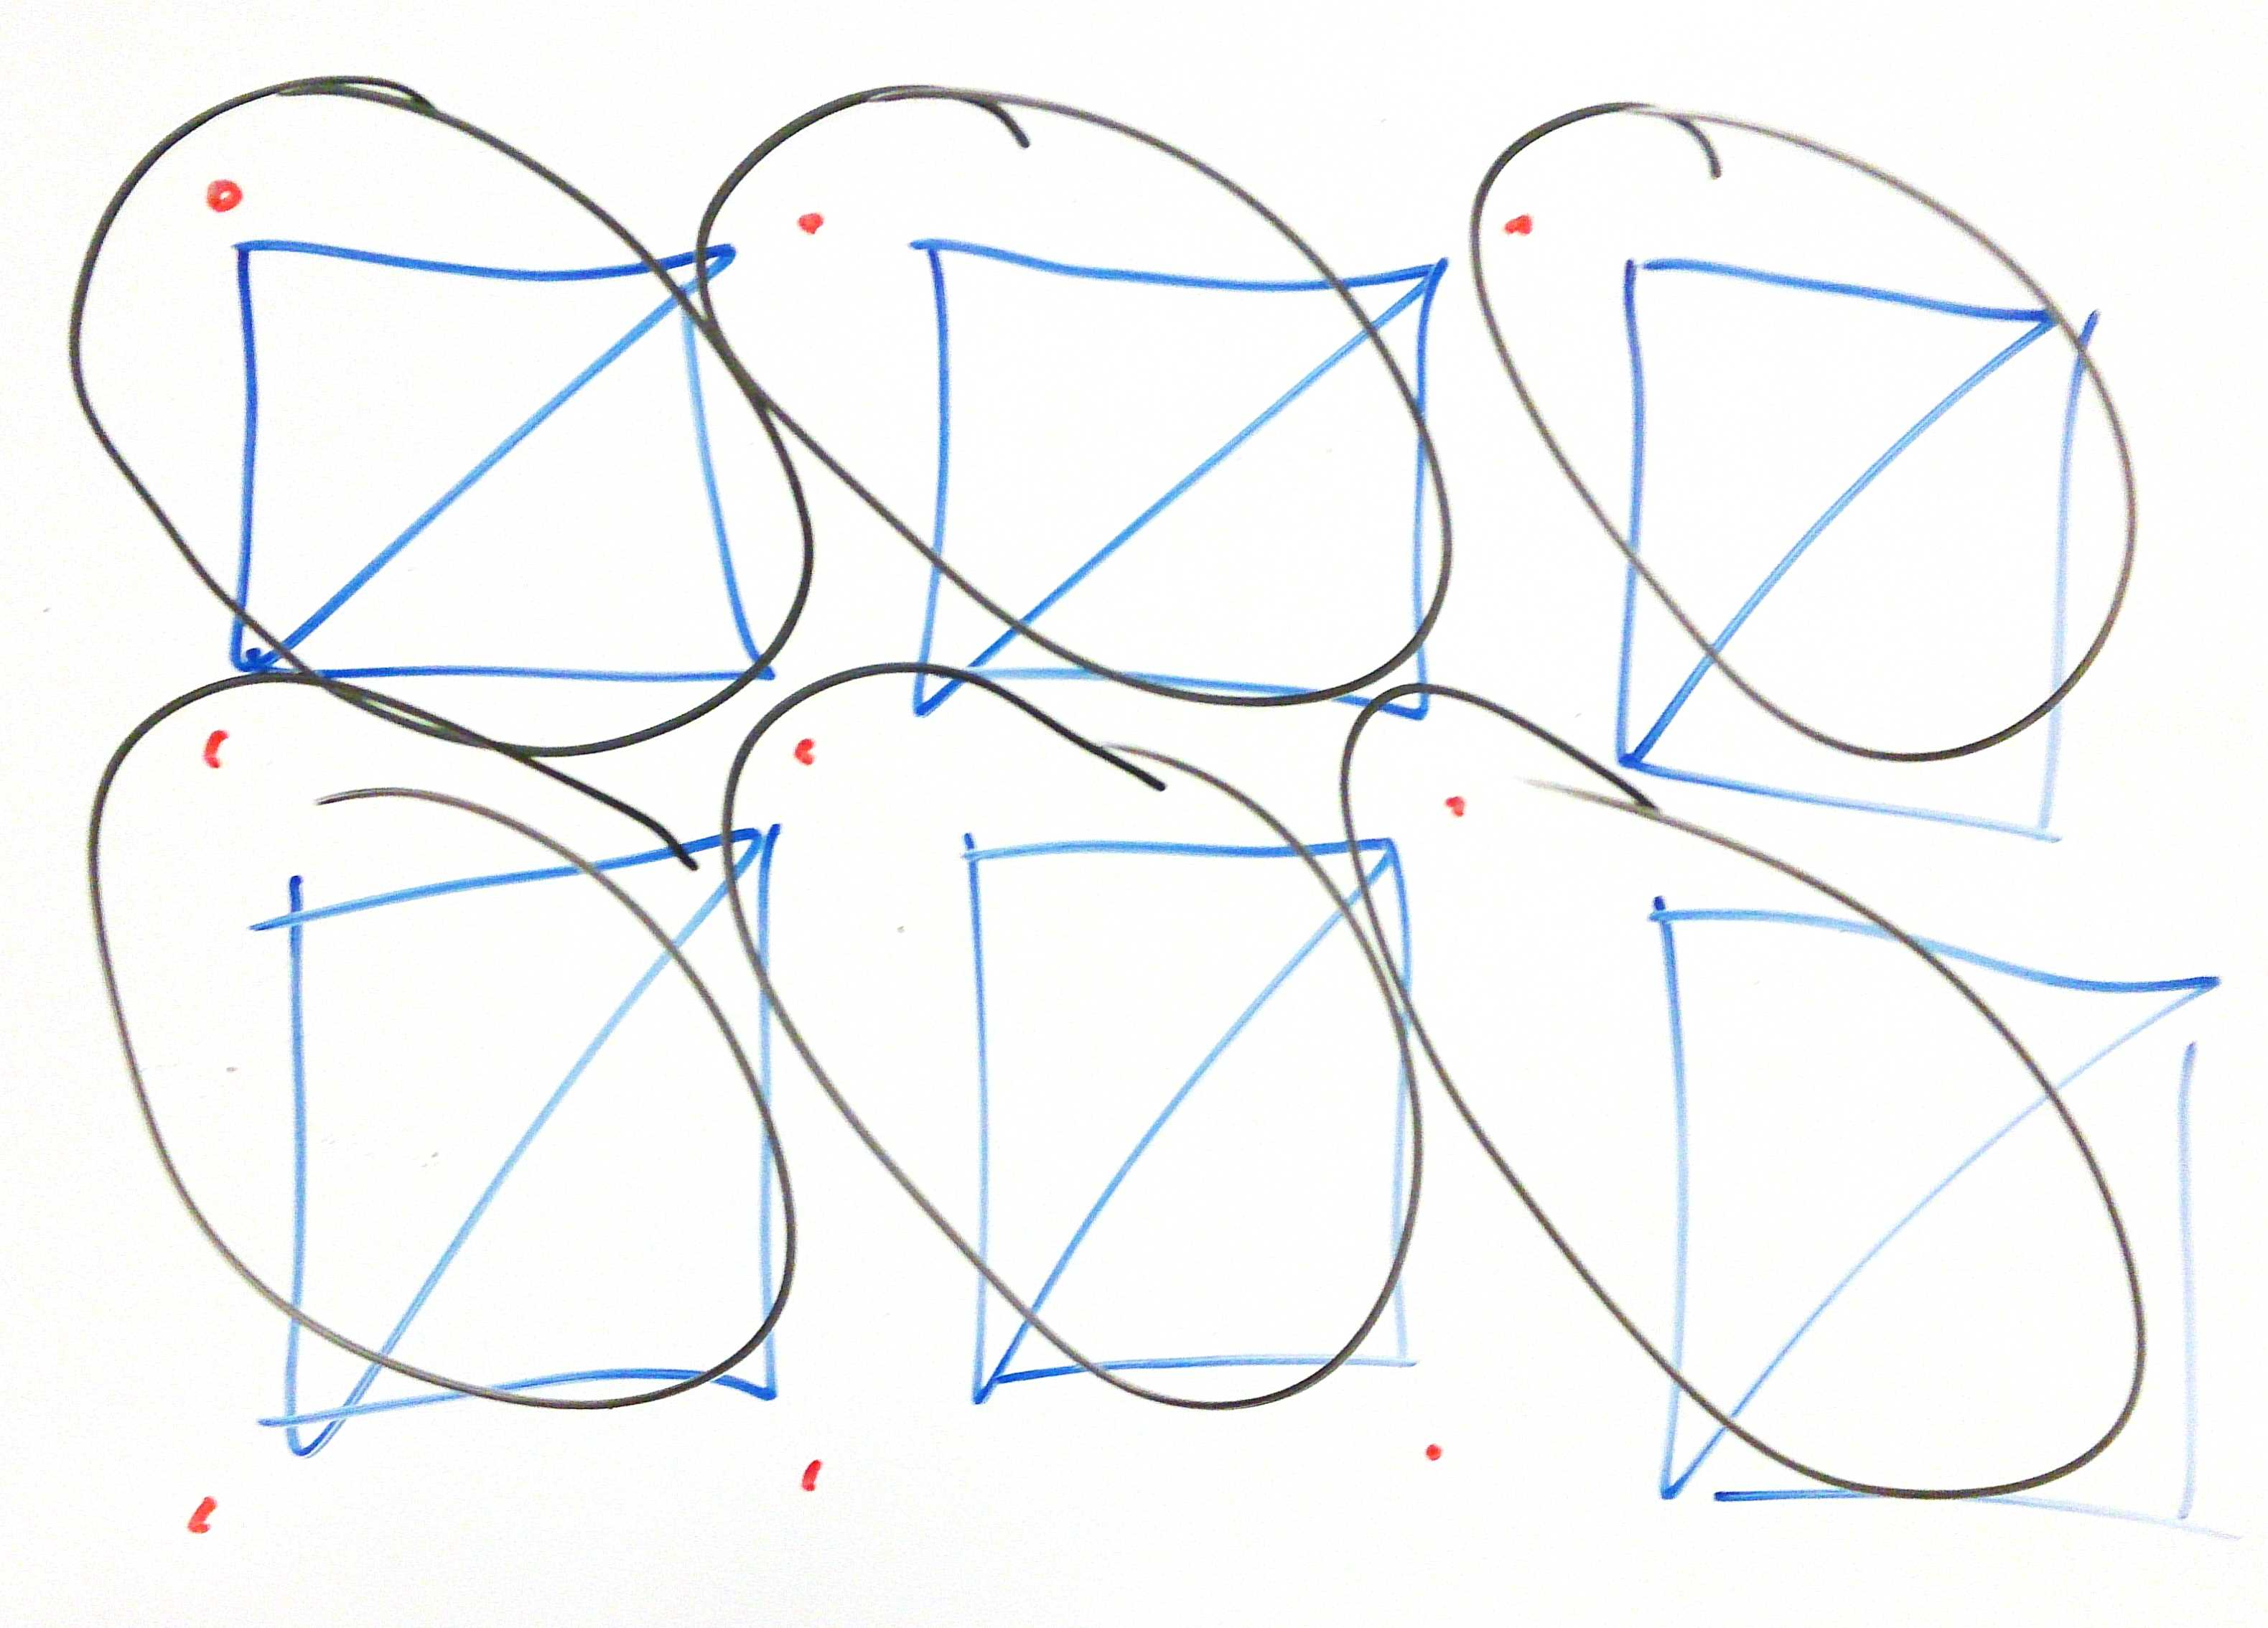
\includegraphics[width=0.6\textwidth]{images/bpa_point_triangle_ratio}
	\caption{
		Explanation for the ratio between mesh size and point cloud size approaching 2.
		If the surface of an object and the corresponding points and triangles are completely unwrapped into a plane, each surface point may be associated with exactly two triangle.
	}
	\label{fig:bpa_point_triangle_ratio}
\end{figure}
%
This correlation now allows to calculate an approximation for the input raycasting resolution given a number of output triangles, which becomes handy if a triangle budget is specified for the output mesh.

The BPA timings in table \ref{tbl:bpa_results}, especially at higher resolutions, further show that the algorithm's runtime is strongly related to the number of points of the cloud.
For each \SI{1}{\kilo\nothing} points, the BPA requires roughly \SI{4}{\milli\second} runtime, emitting \SI{2}{\kilo\nothing} triangles.
At lower resolutions, the overhead of the parallelization becomes visible, which is not as straight-forward as for the embarrassingly parallel tri-dexel or direct intersection, \cf the corresponding paper \cite{bpa_vml}.

Concerning memory demands, the BPA requires quite a bit of space for its acceleration structure, a regular grid partitioning the point cloud.
This grid greatly speeds up the search for nearby points during pivoting.
Furthermore, this grid is also the basis for a parallelization, \cf the corresponding paper for details \cite{bpa_vml}.
In addition to the grid, the currently built mesh is stored in a rich data structure, maintaining not only triangles but also a lot of connectivity information between vertices, edges and faces.
These data structures sum up to roughly \SI{1.2}{\gibi\byte} memory during a reconstruct of the impeller at a resolution of 400.

Figure \ref{fig:bpa_results} shows renderings of the result meshes after running the VML's BPA on point clouds created with a resolution of 400.
%
\begin{figure}
	\centering
	\begin{subfigure}[b]{0.34\textwidth}
		\centering
		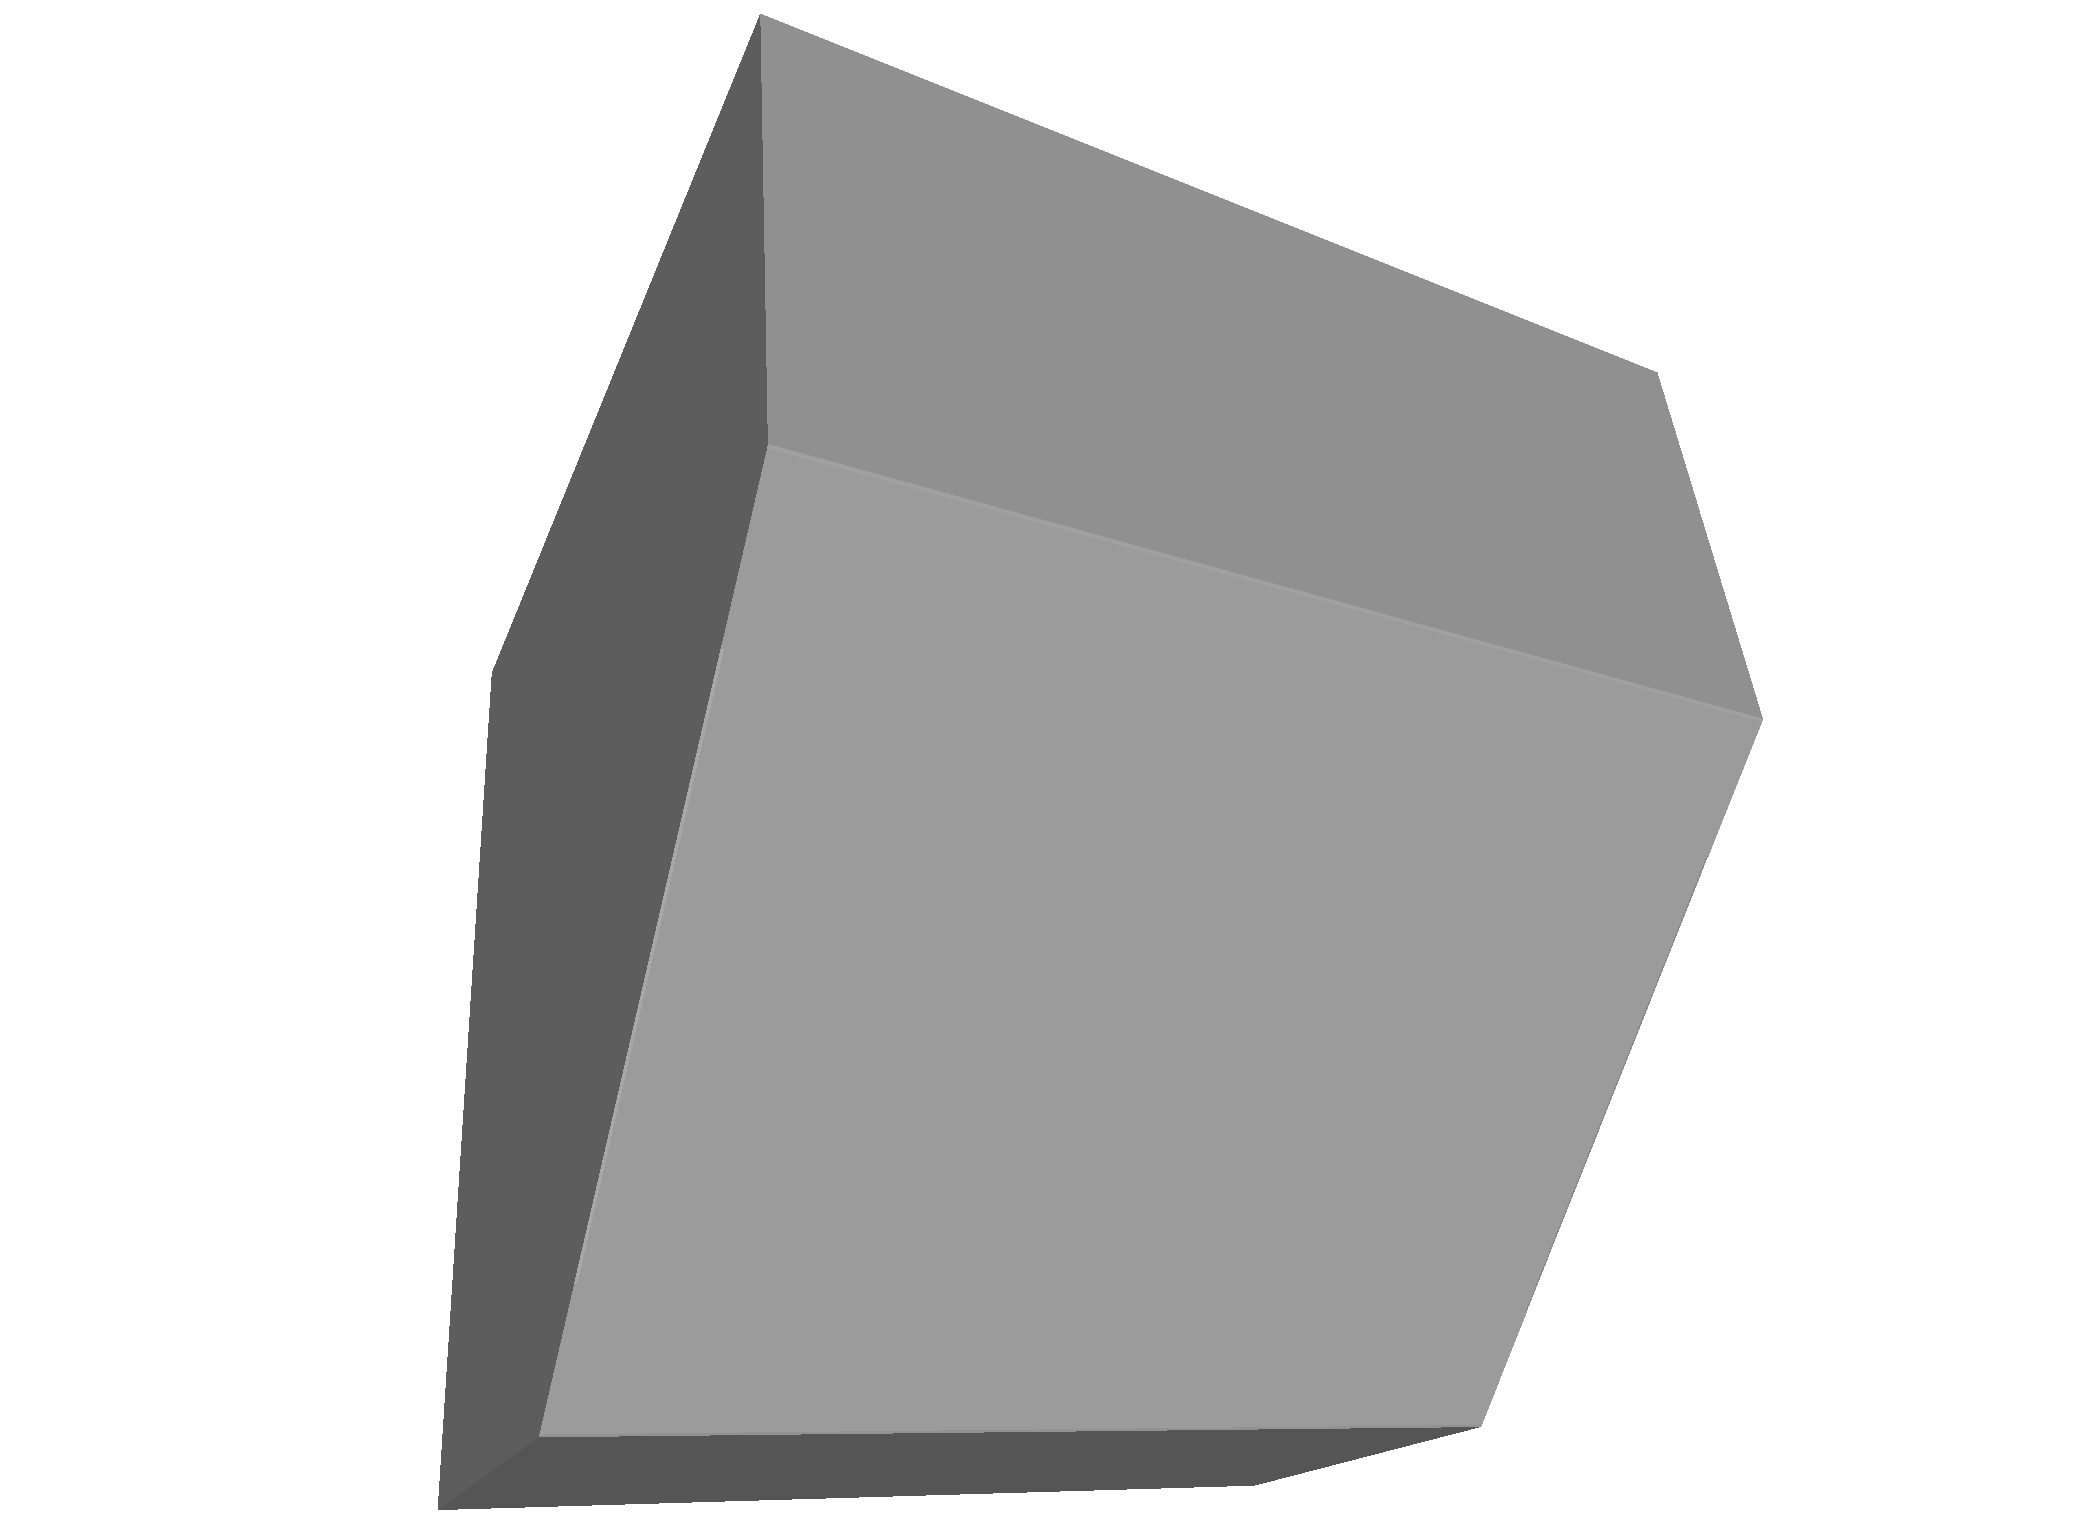
\includegraphics[width=\textwidth]{bpa_cube2}
		\caption{cube2}
		\label{fig:bpa_cube2}
	\end{subfigure}
	\hspace{1cm}
	\begin{subfigure}[b]{0.34\textwidth}
		\centering
		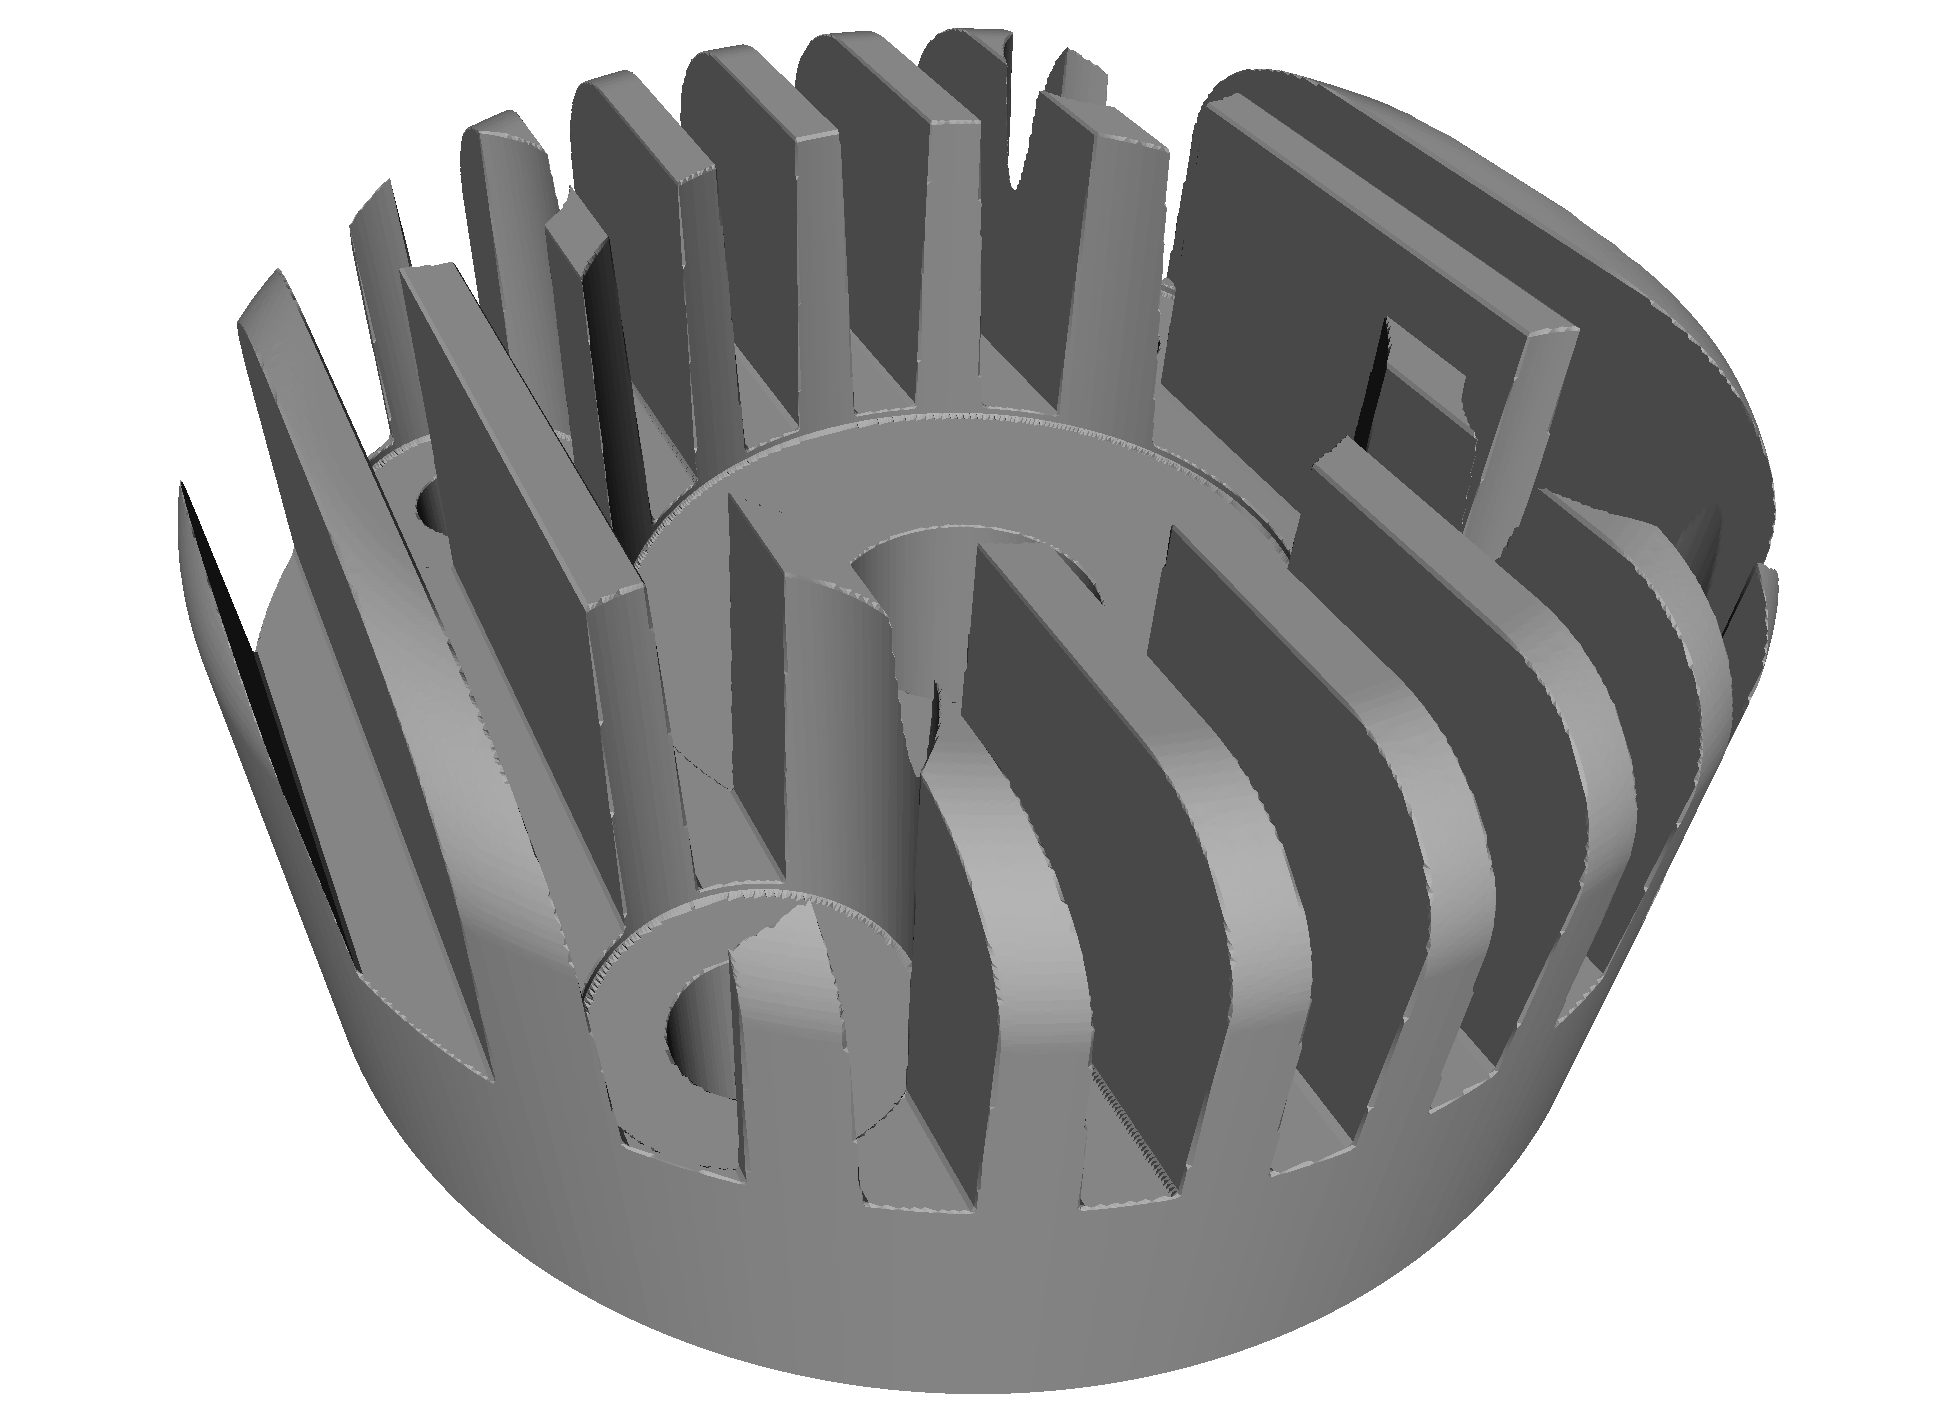
\includegraphics[width=\textwidth]{bpa_cylinder_head}
		\caption{cylinder\_head}
		\label{fig:bpa_cylinder_head}
	\end{subfigure}
	\begin{subfigure}[b]{0.34\textwidth}
		\centering
		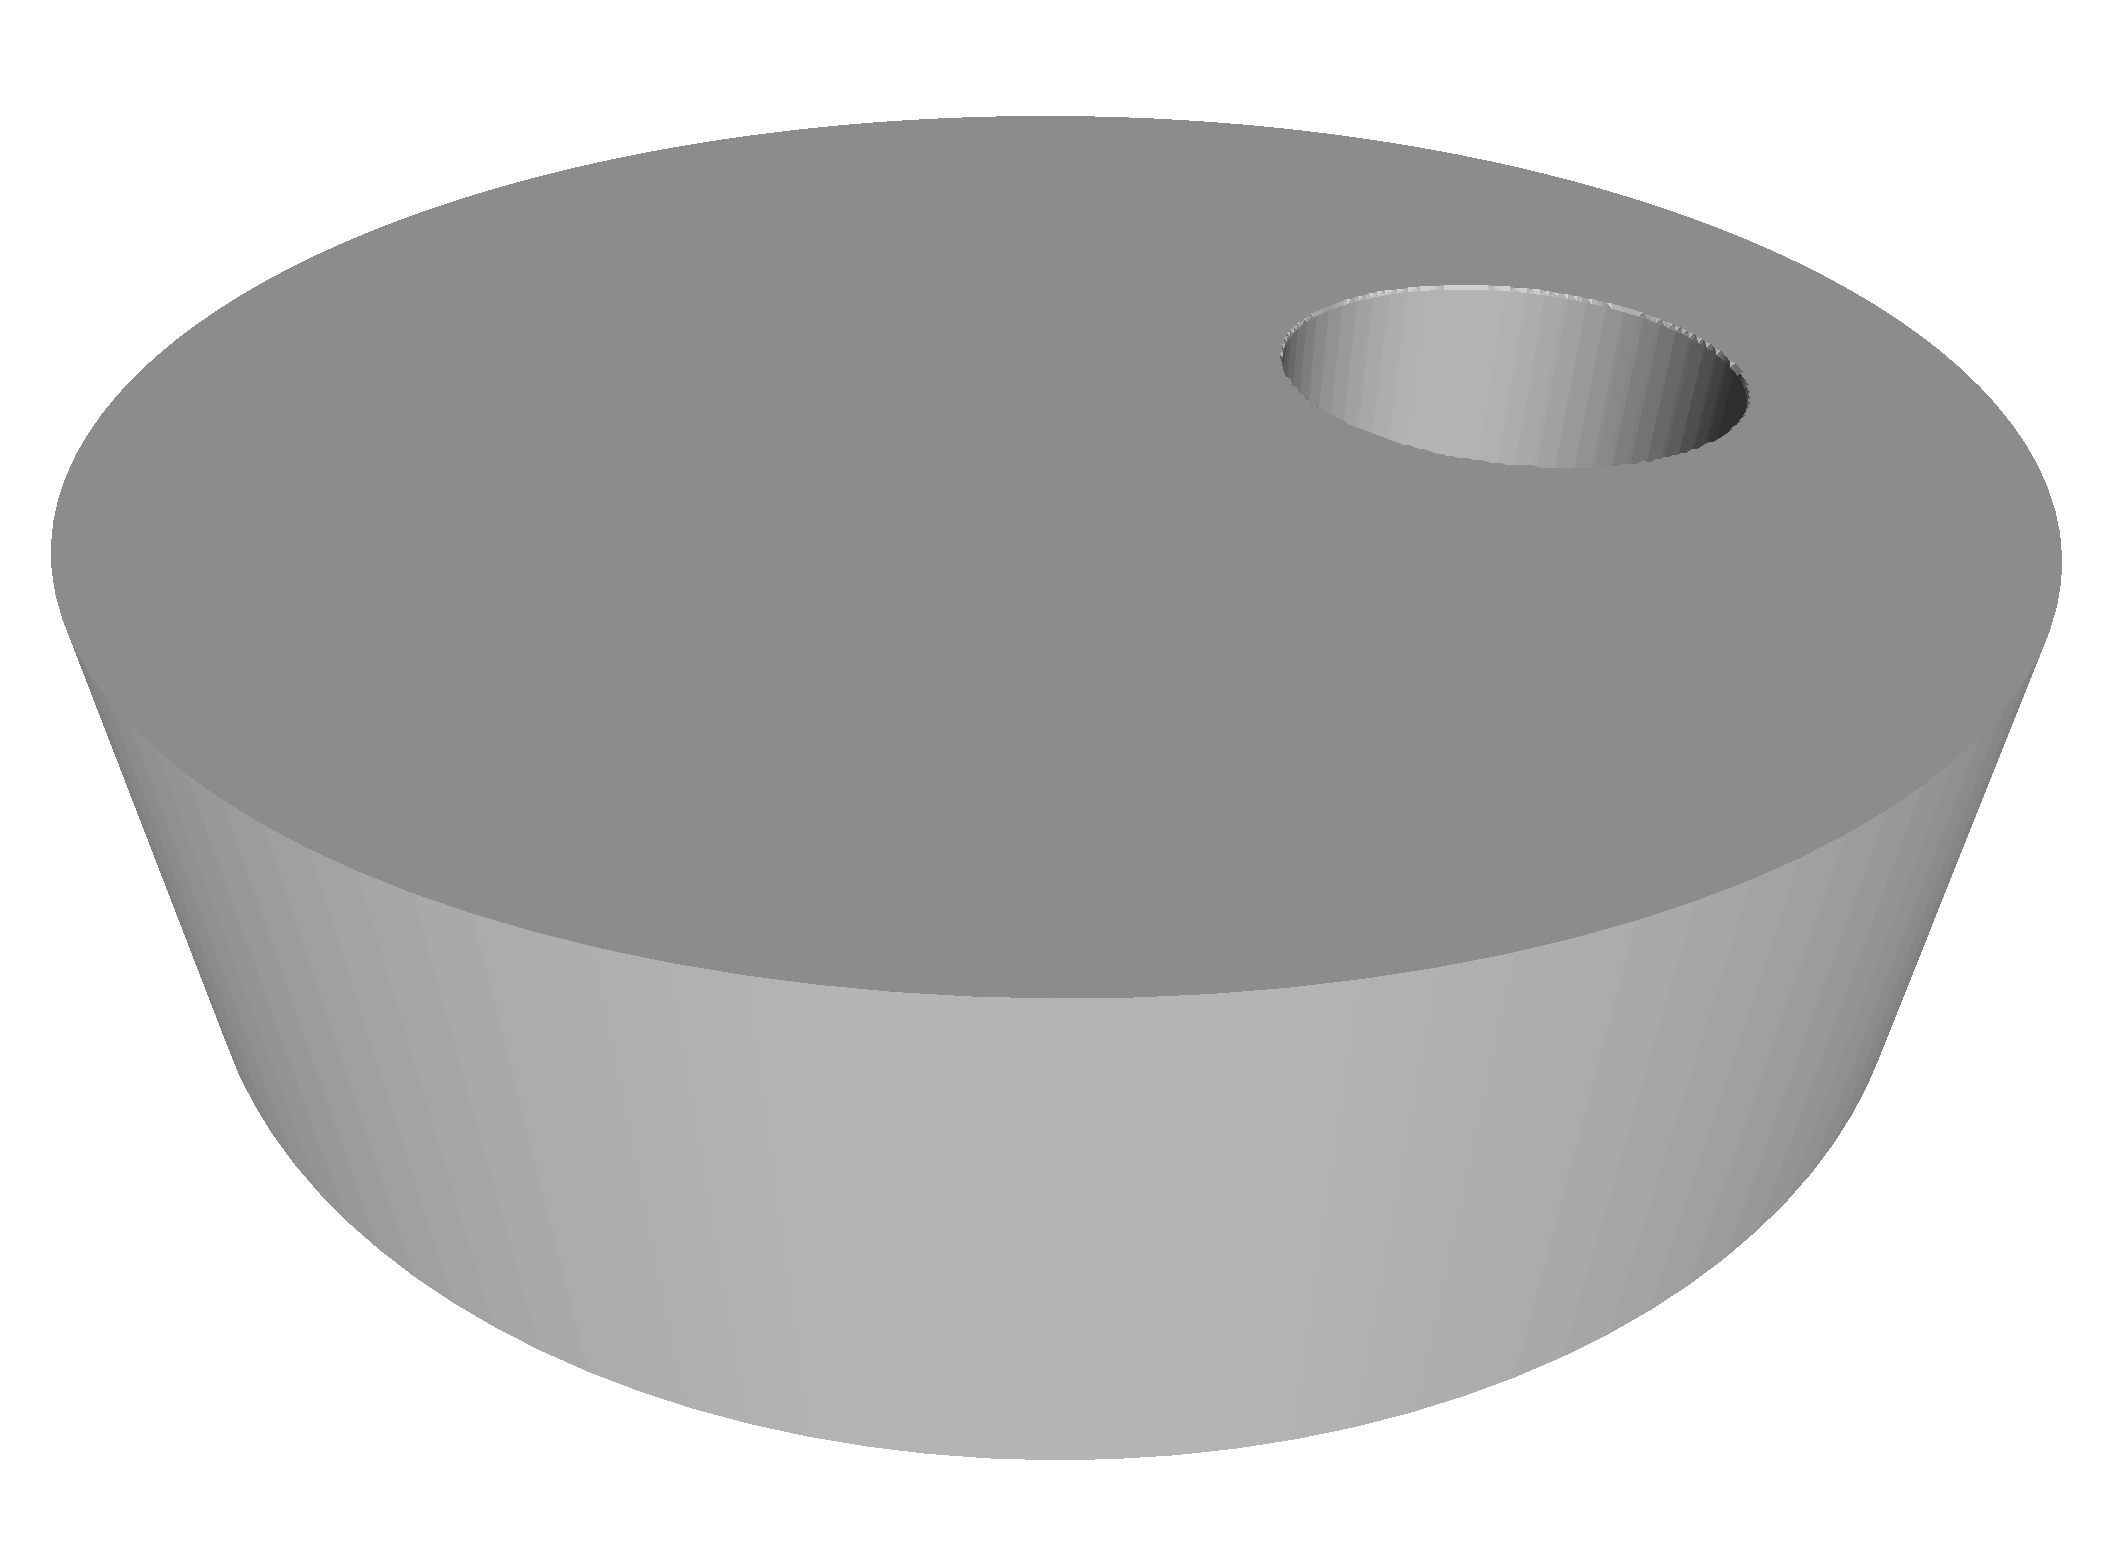
\includegraphics[width=\textwidth]{bpa_cylinders}
		\caption{cylinders}
		\label{fig:bpa_cylinders}
	\end{subfigure}
	\hspace{1cm}
	\begin{subfigure}[b]{0.34\textwidth}
		\centering
		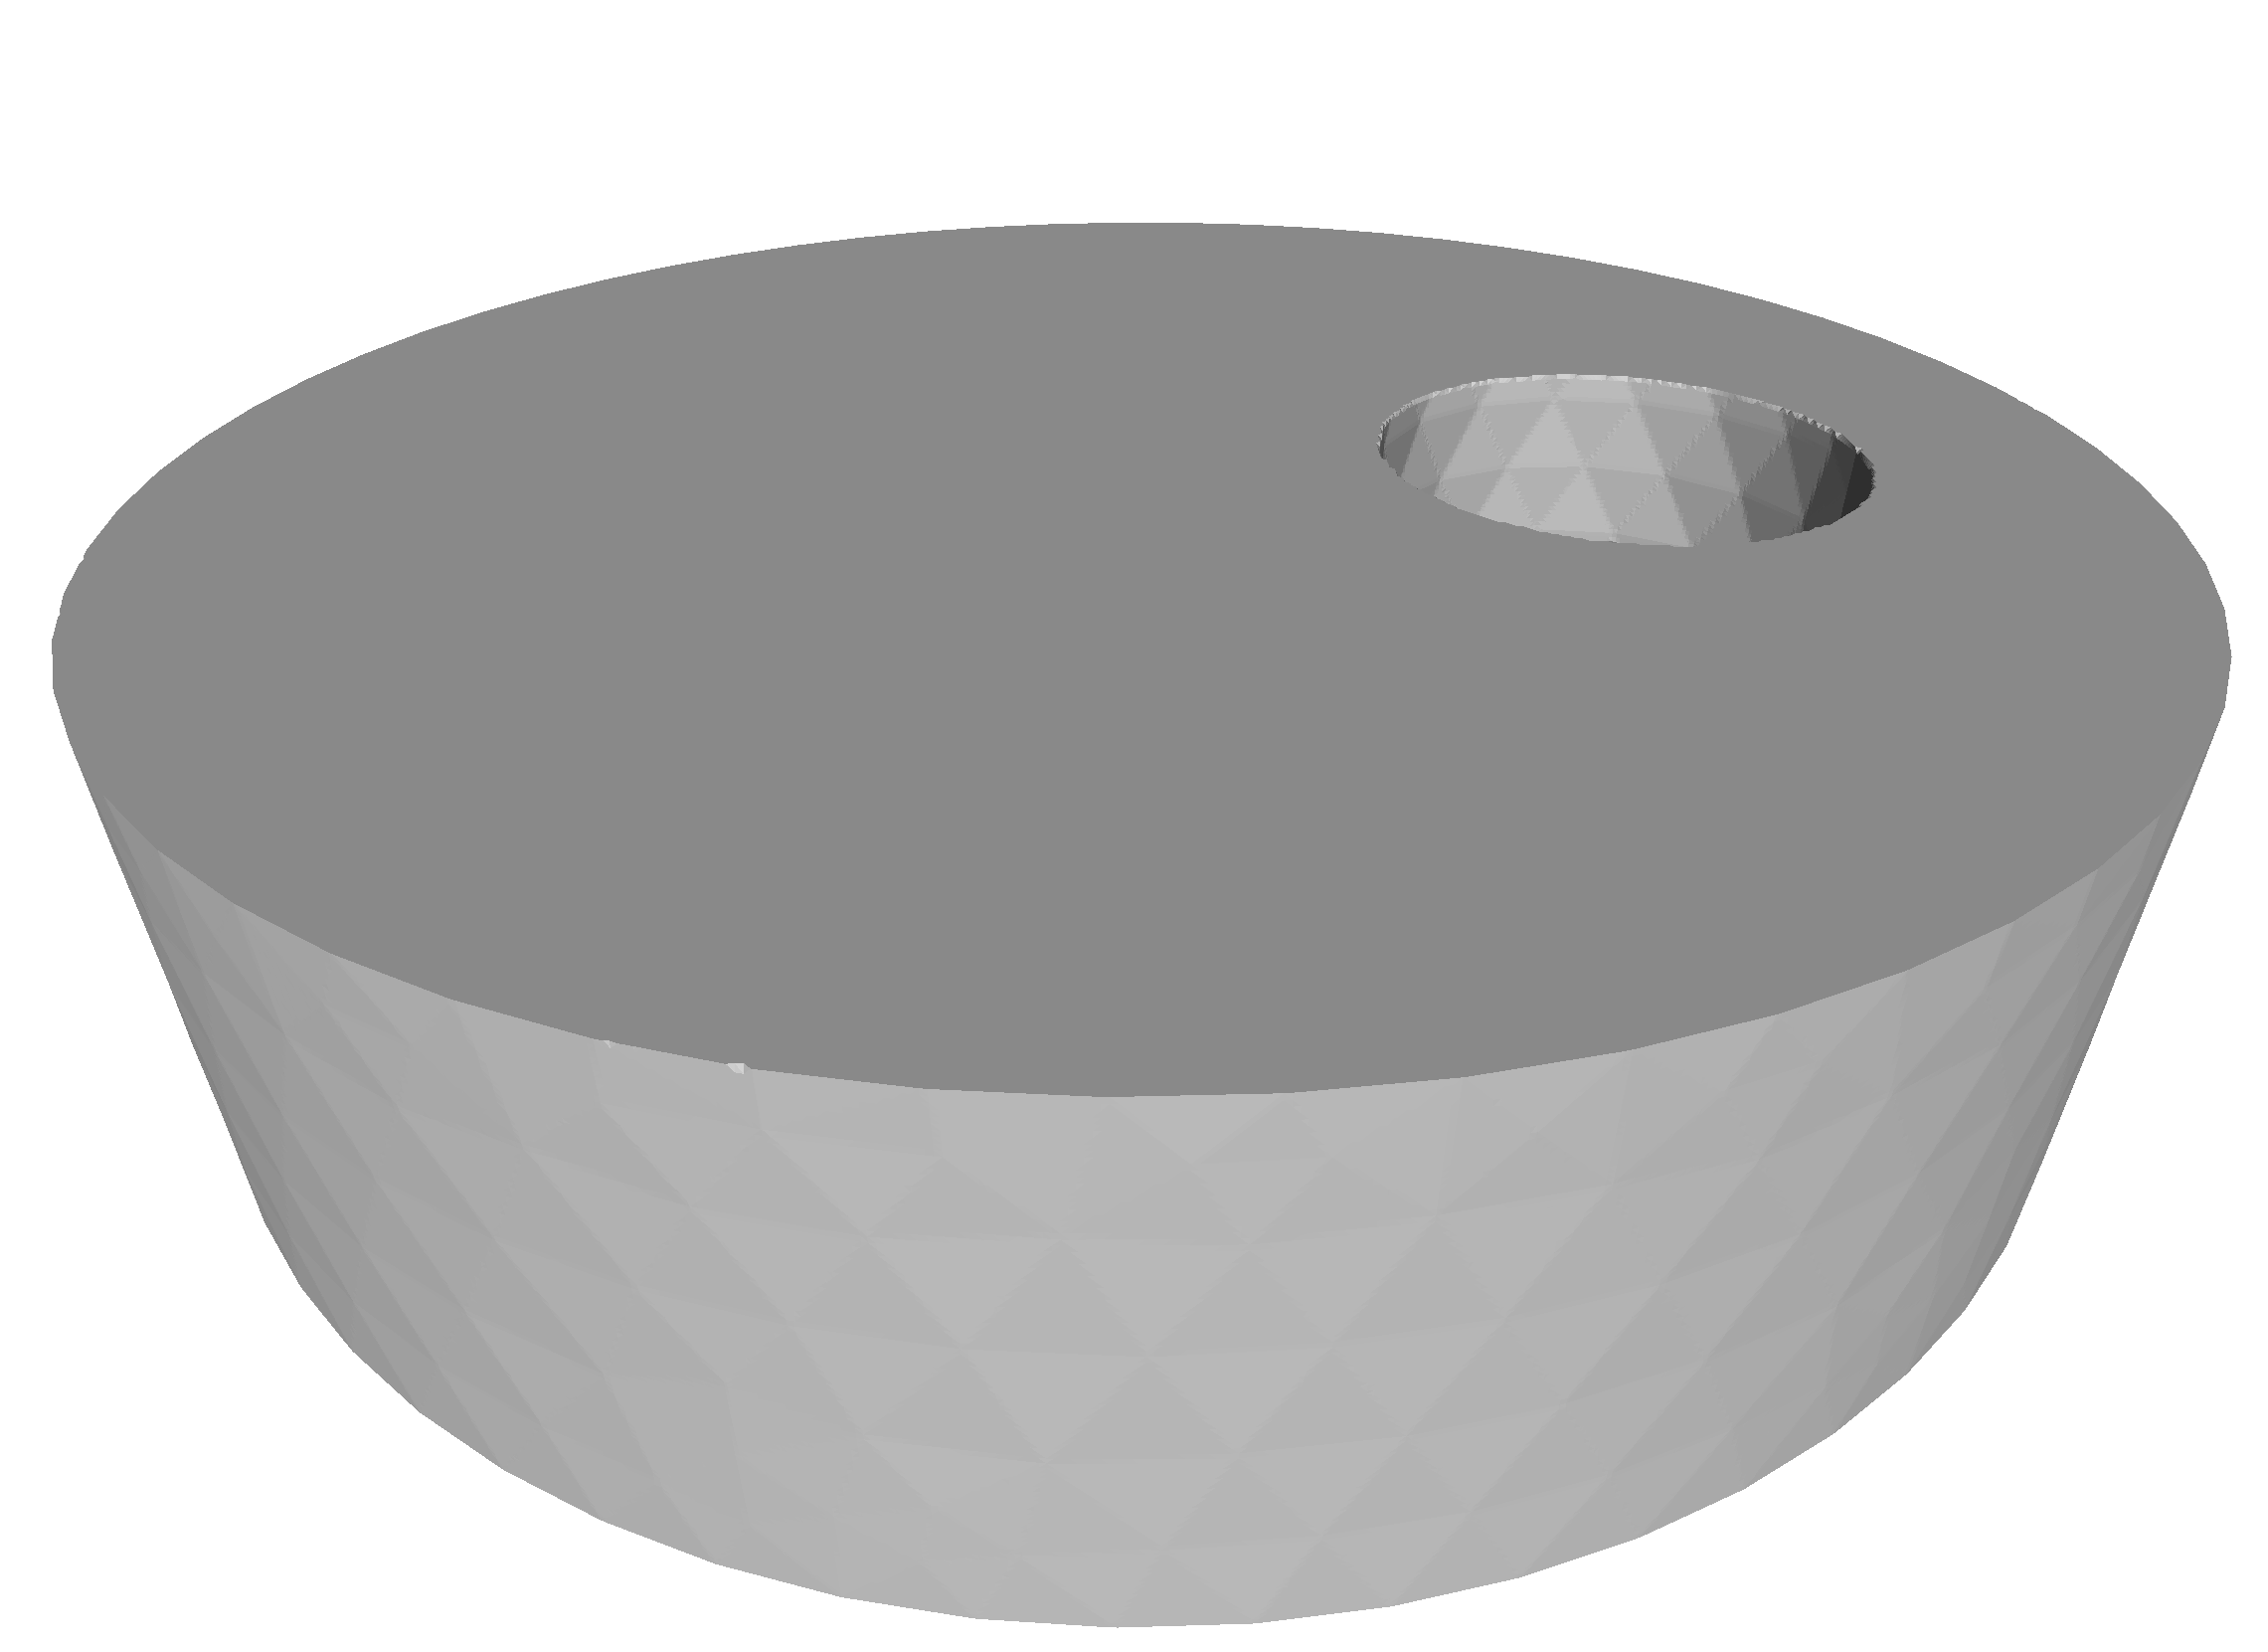
\includegraphics[width=\textwidth]{bpa_cylinders_d}
		\caption{cylinders\_d}
		\label{fig:bpa_cylinders_d}
	\end{subfigure}
	\begin{subfigure}[b]{0.34\textwidth}
		\centering
		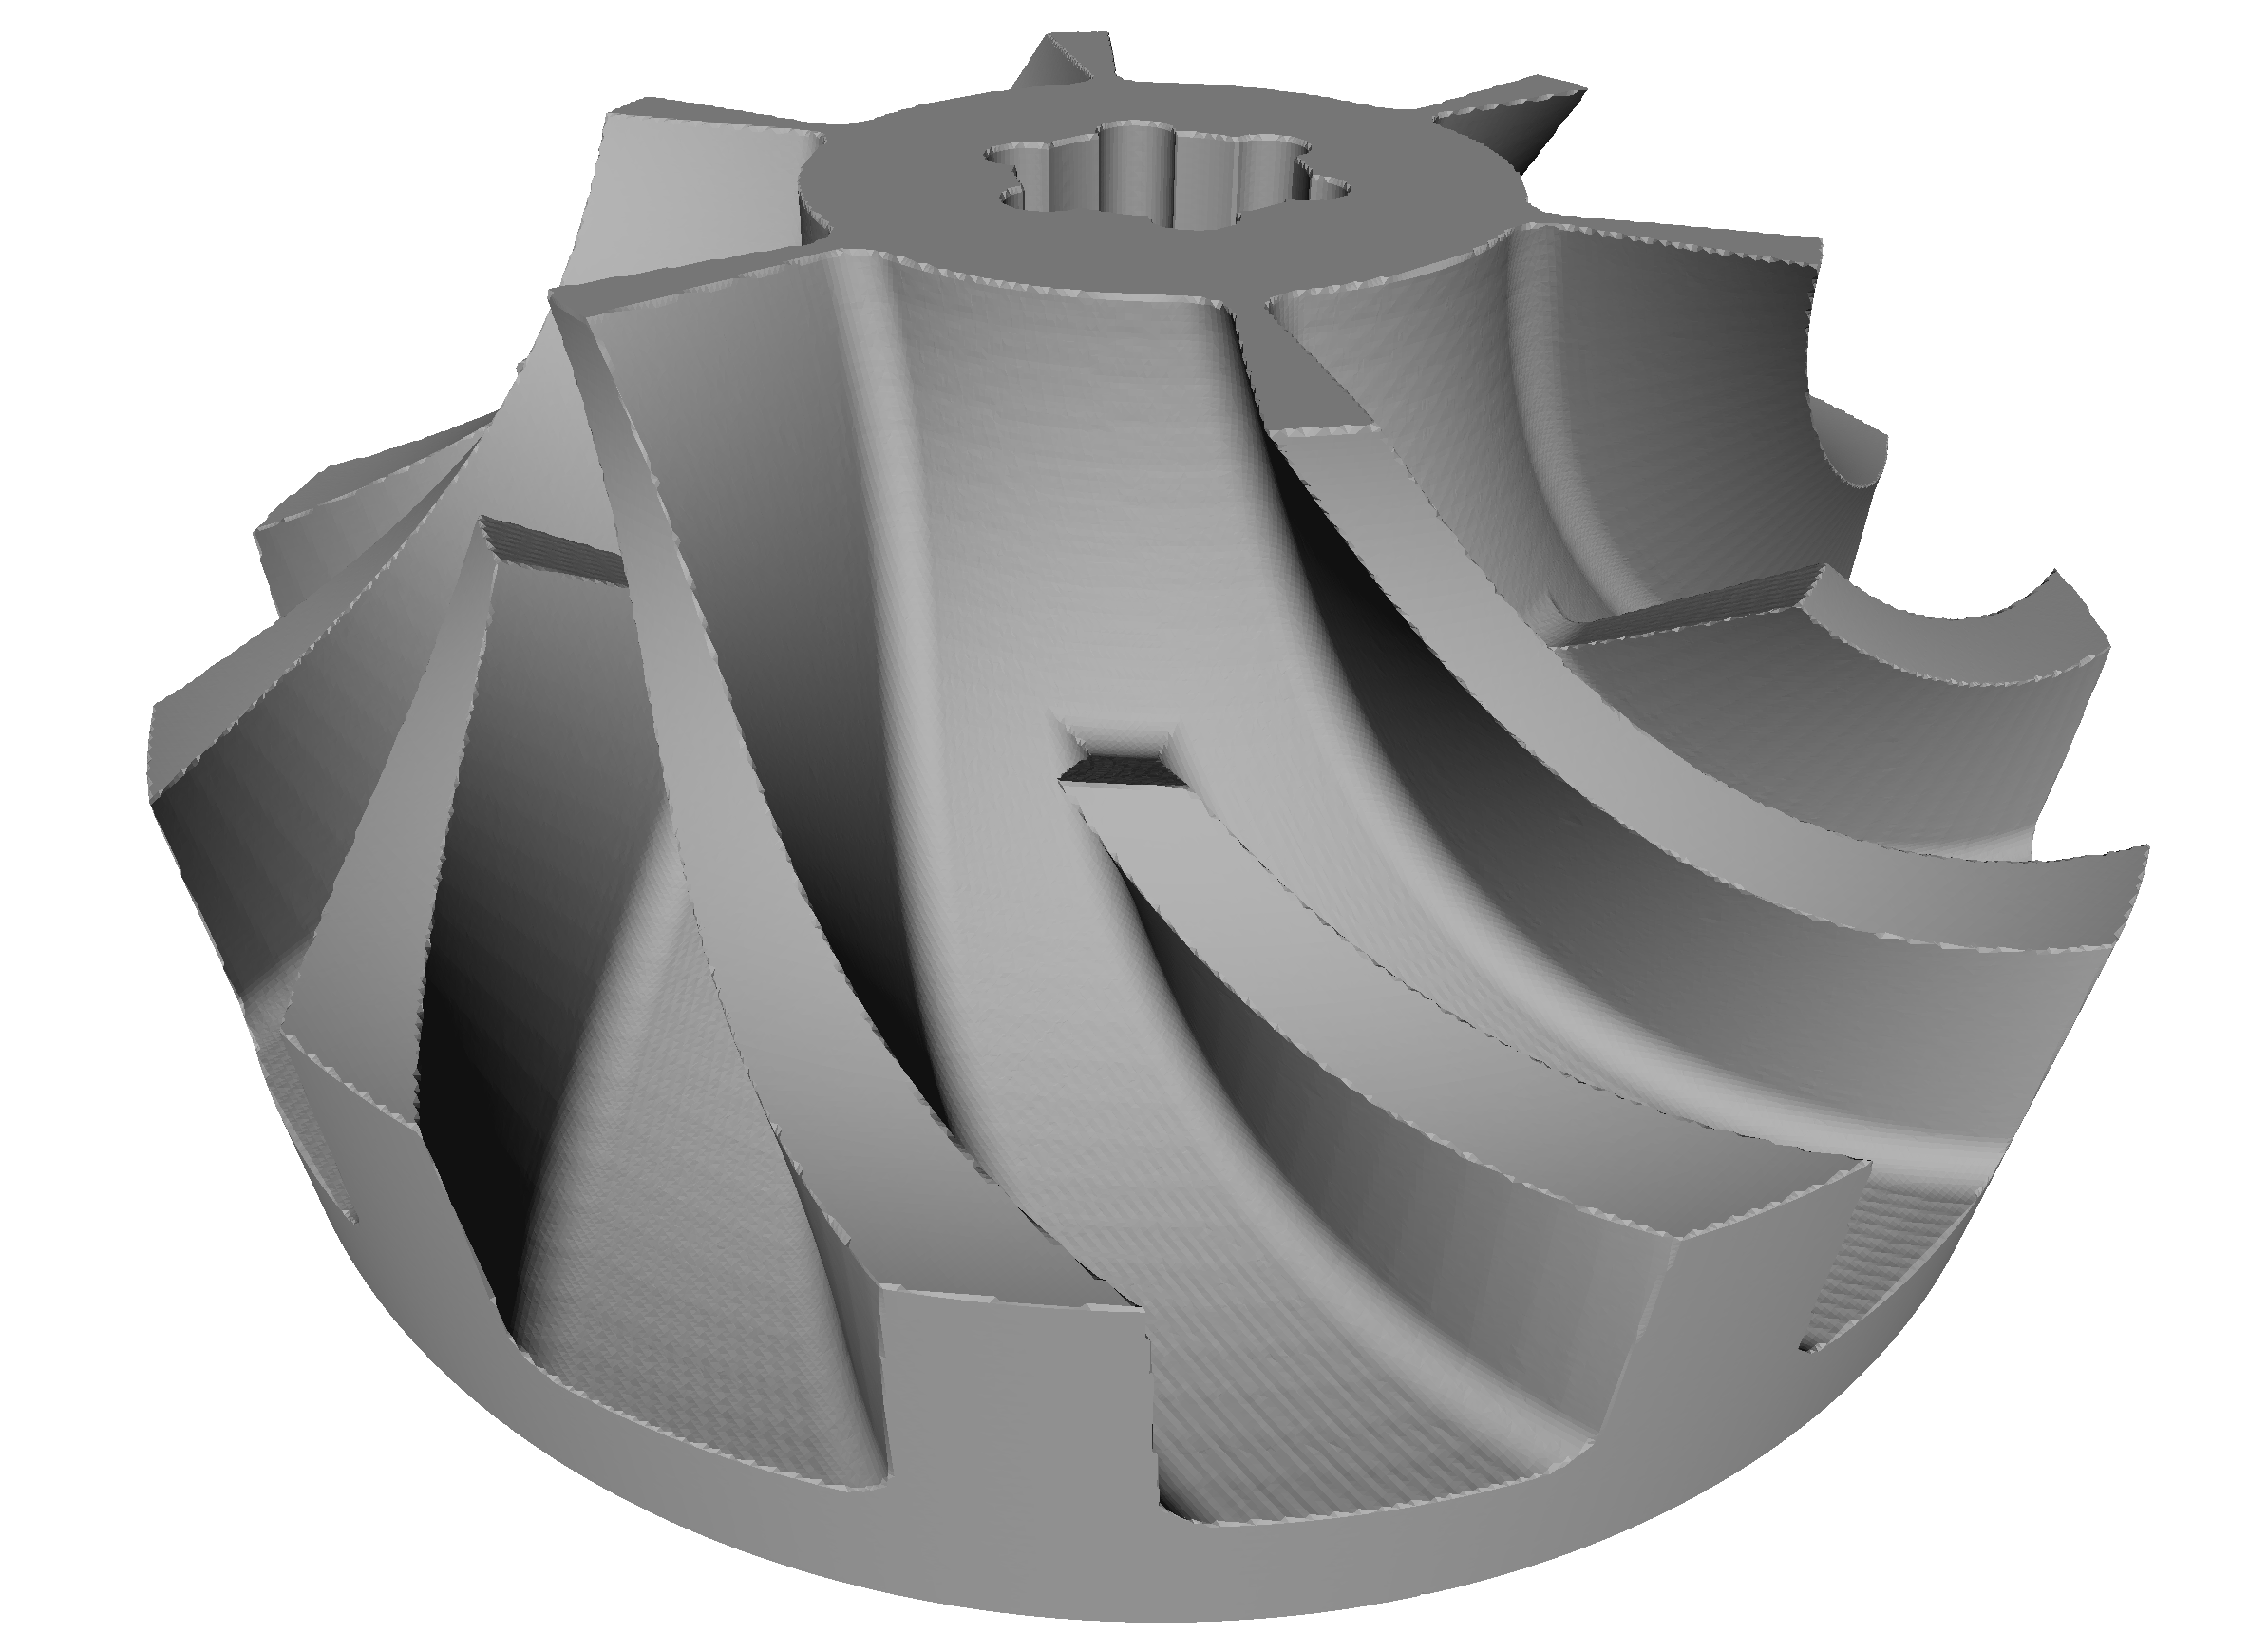
\includegraphics[width=\textwidth]{bpa_hq_impeller}
		\caption{impeller}
		\label{fig:bpa_hq_impeller}
	\end{subfigure}
	\hspace{1cm}
	\begin{subfigure}[b]{0.34\textwidth}
		\centering
		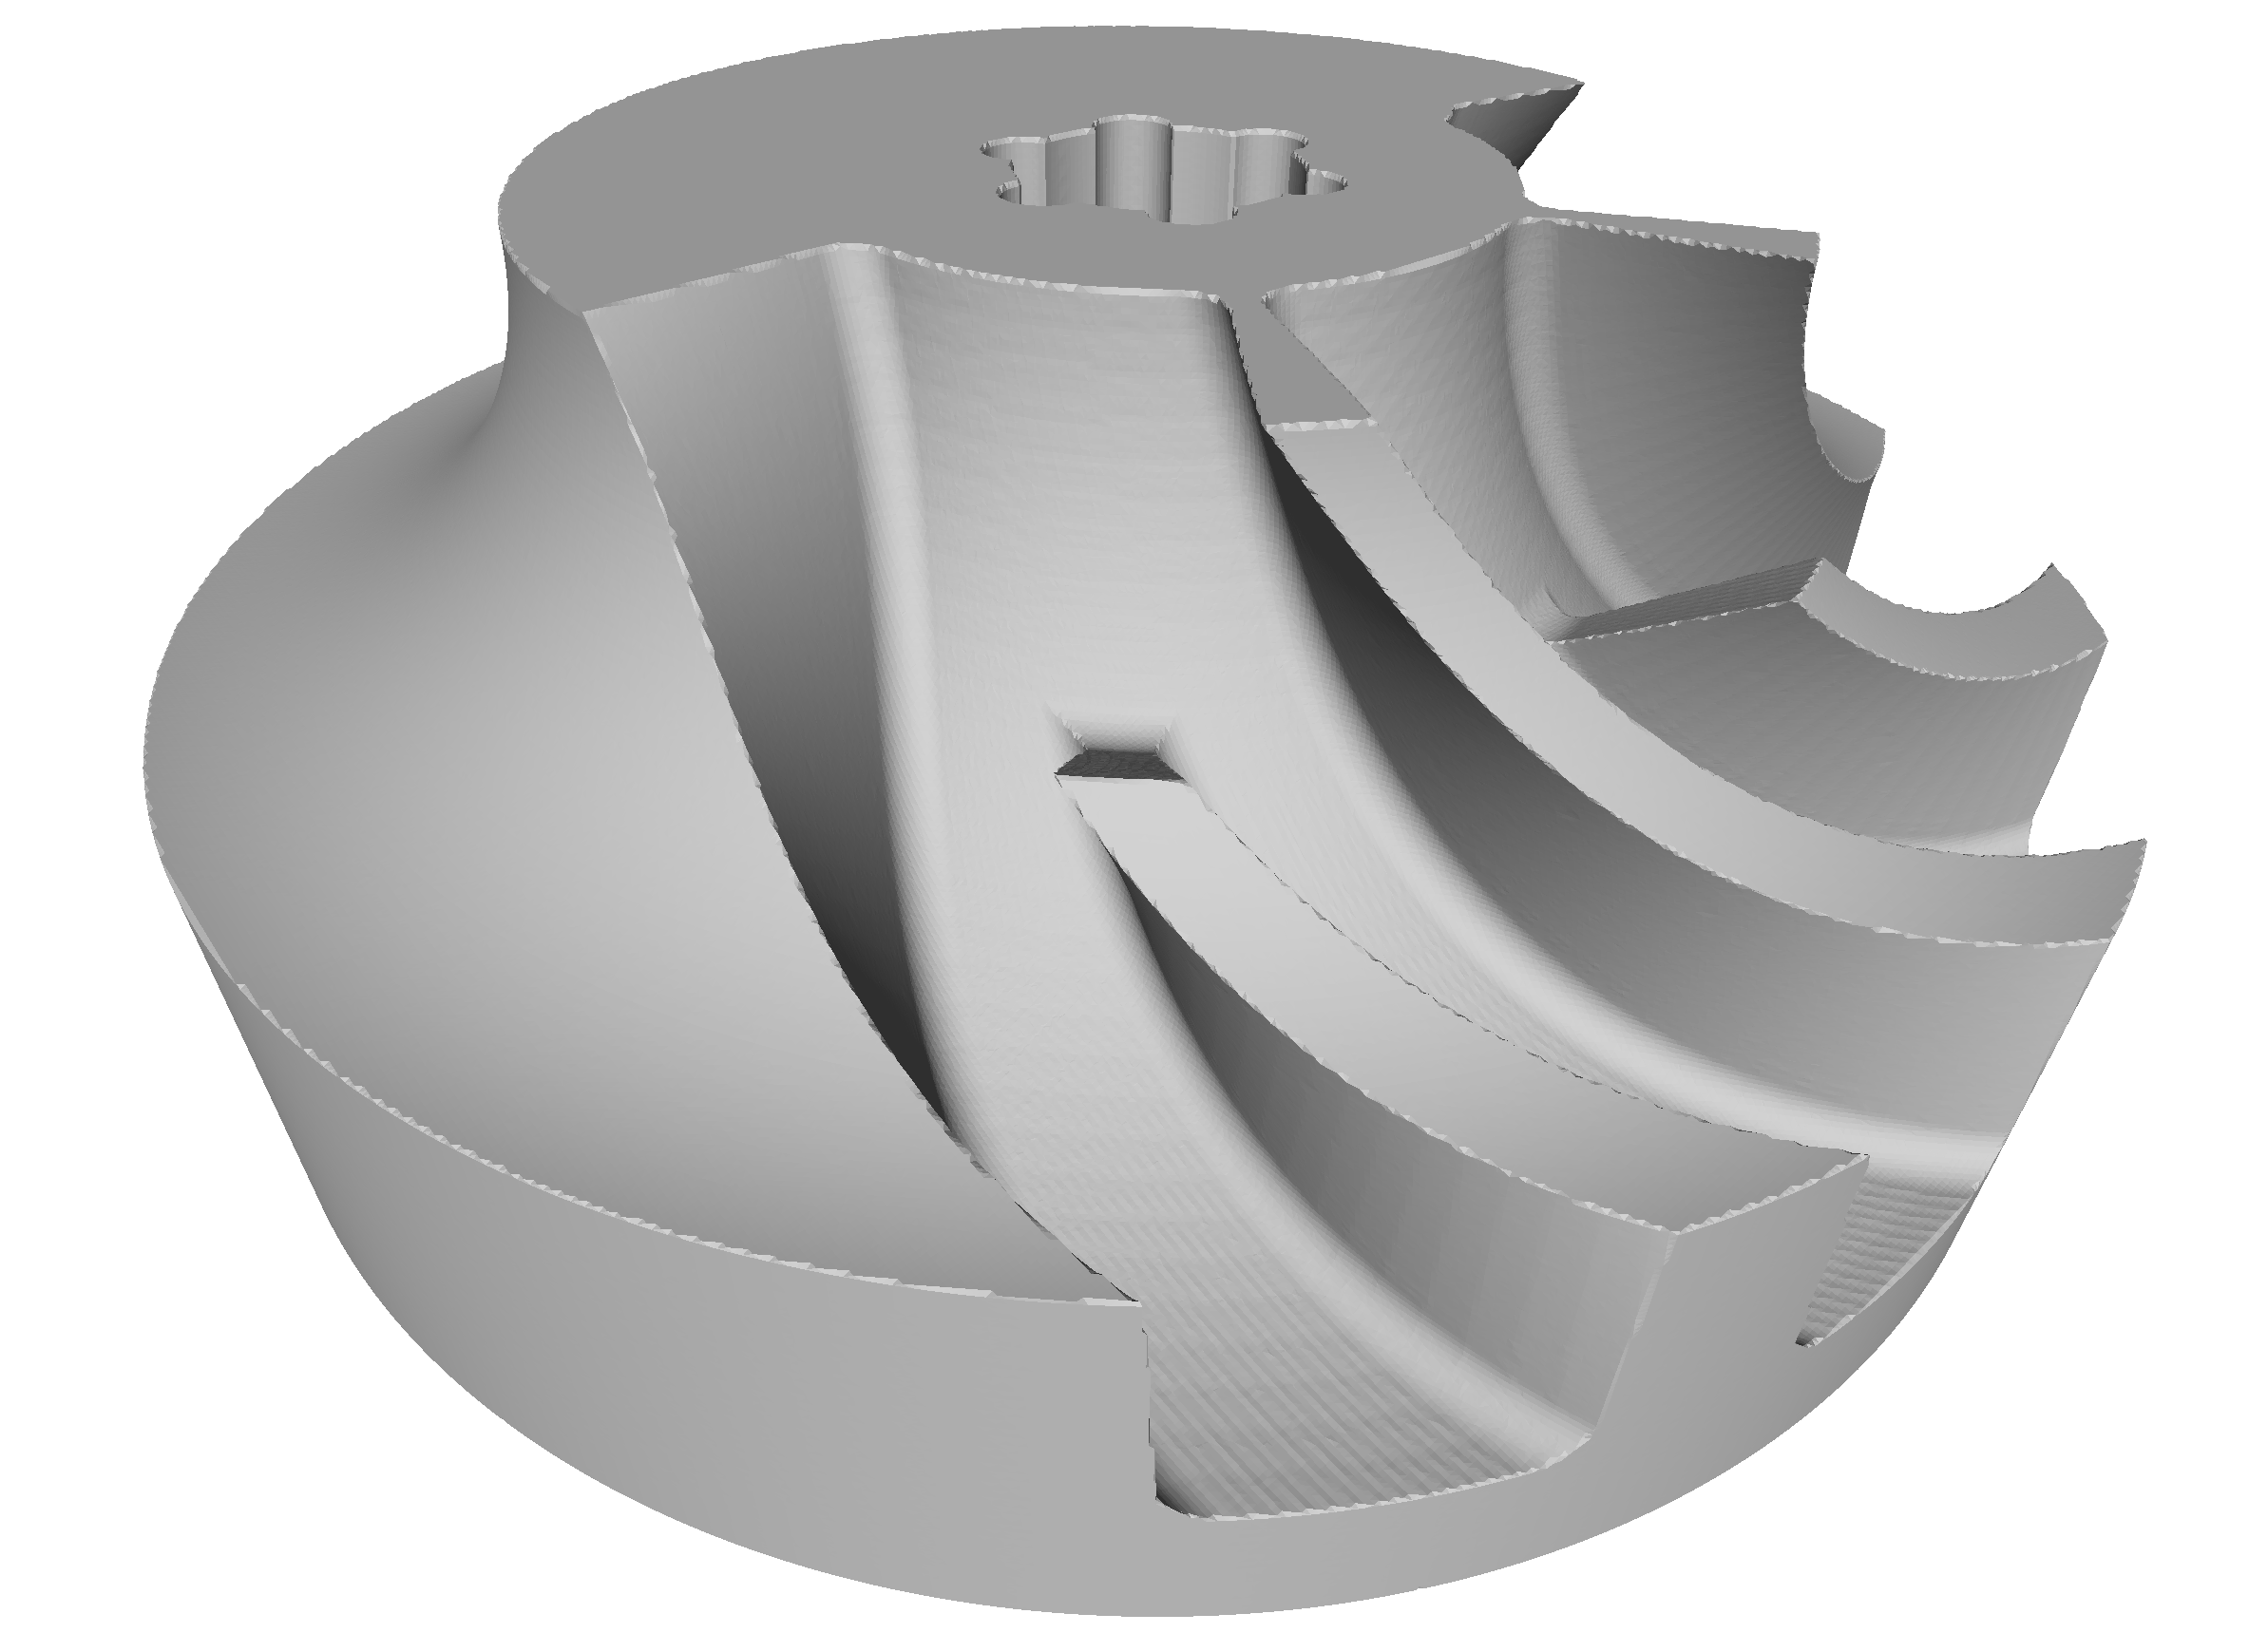
\includegraphics[width=\textwidth]{bpa_hq_impeller_2}
		\caption{impeller\_2}
		\label{fig:bpa_hq_impeller_2}
	\end{subfigure}
	\begin{subfigure}[b]{0.33\textwidth}
		\centering
		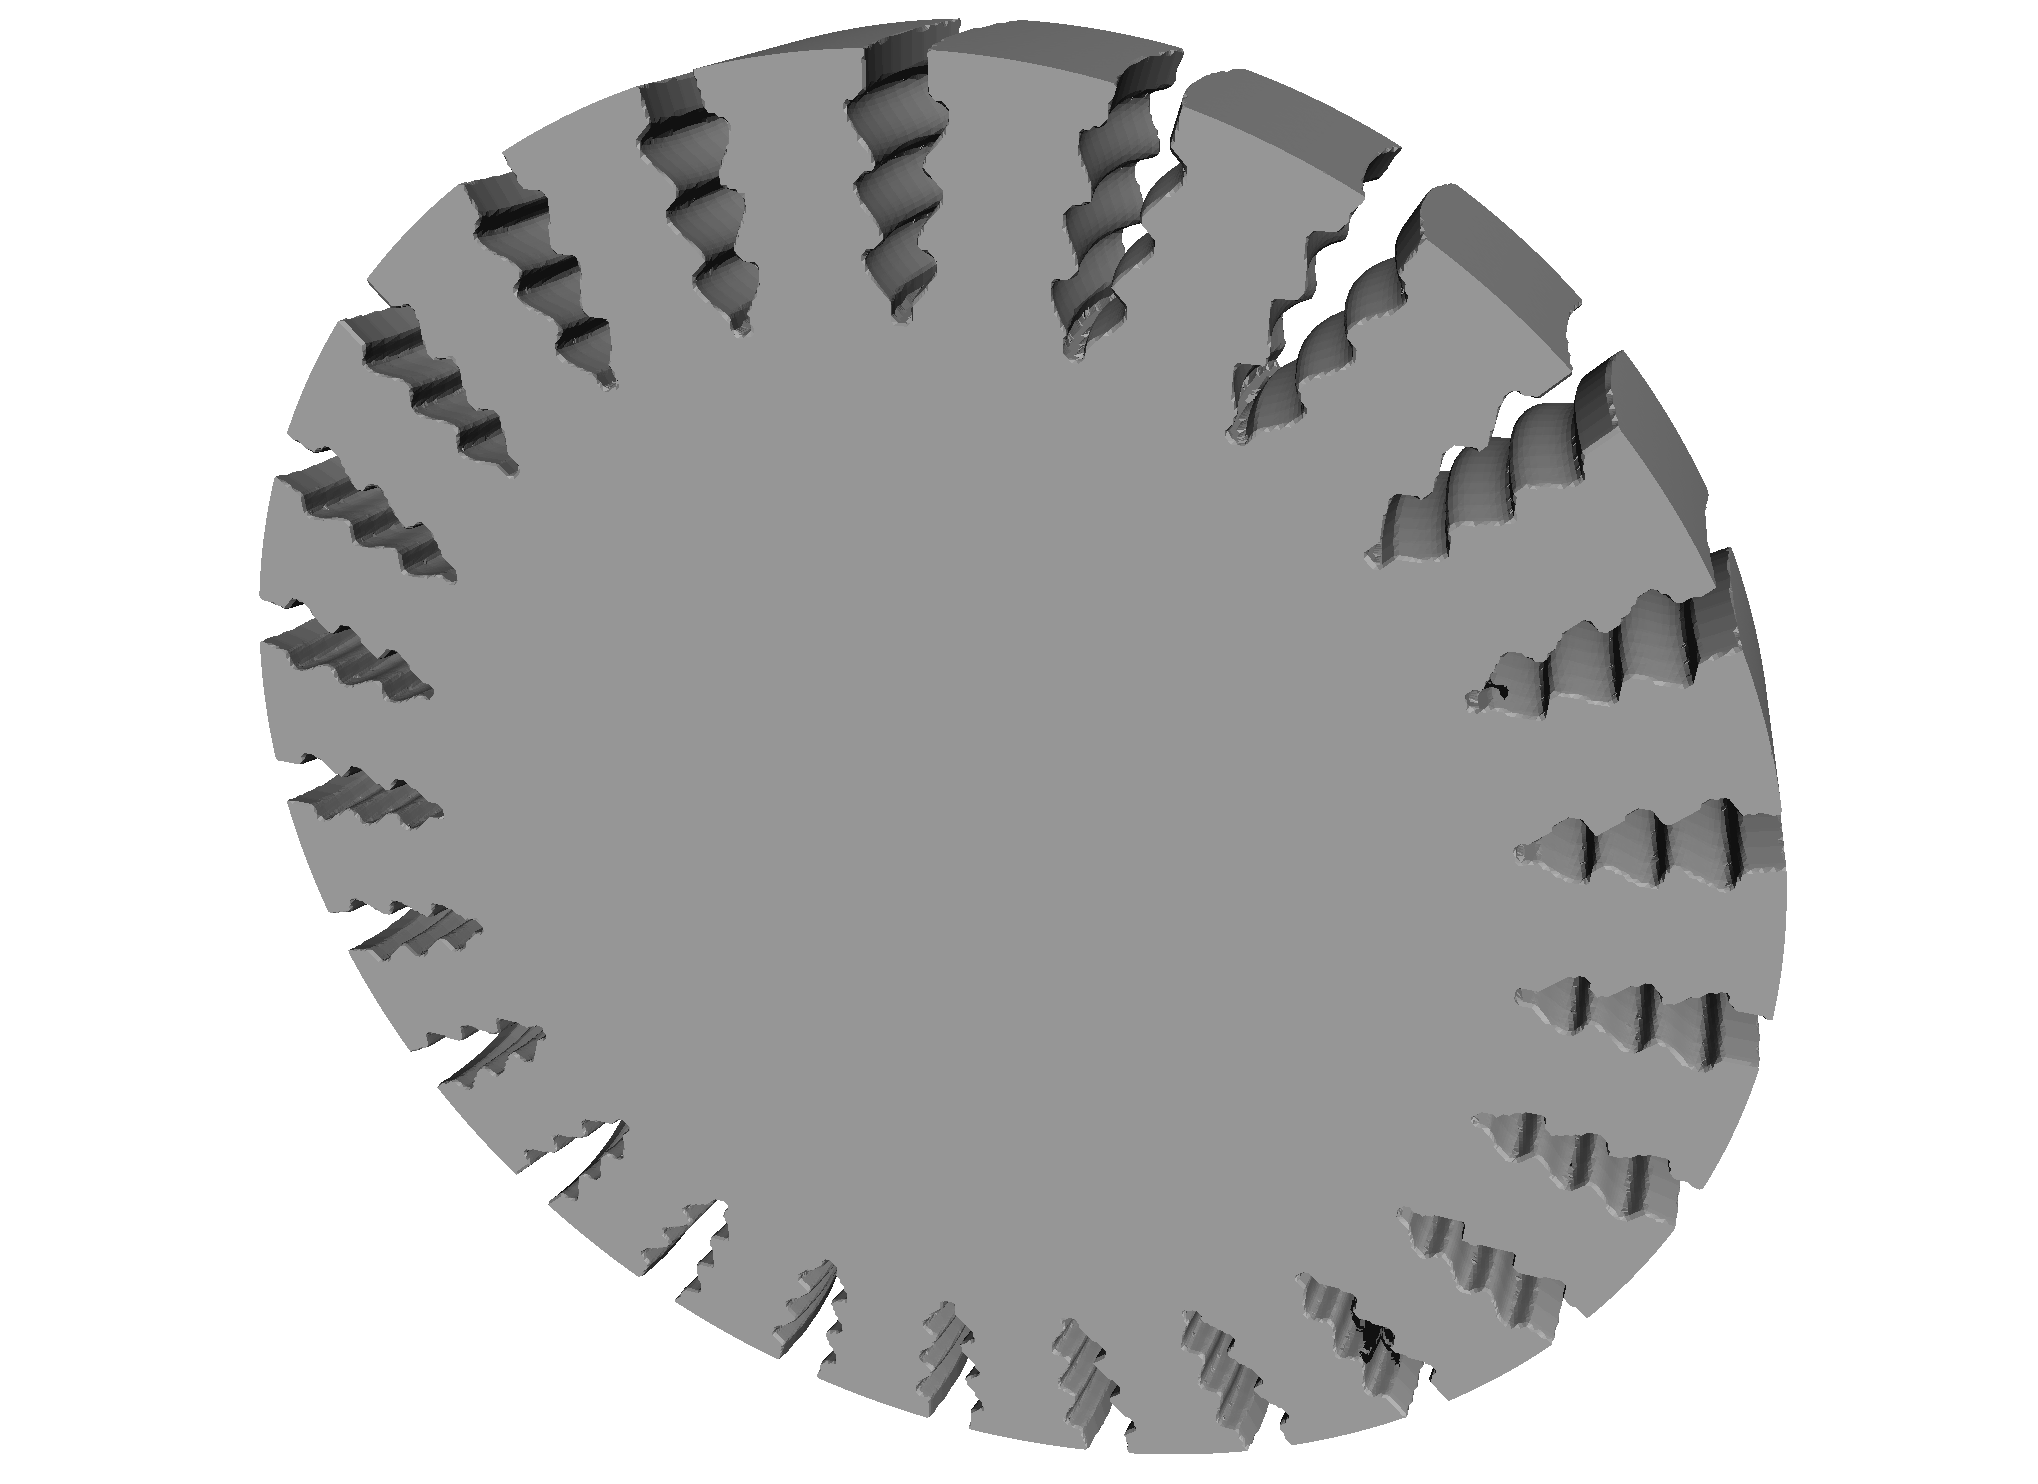
\includegraphics[width=\textwidth]{bpa_turbine}
		\caption{turbine}
		\label{fig:bpa_turbine}
	\end{subfigure}
	\caption{
		Renderings of the result meshes using MeshLab after applying the BPA reconstruction approach on a point cloud created with a resolution of 400 on the selected test scenes in table \ref{tbl:test_scenes}.
	}
	\label{fig:bpa_results}
\end{figure}
%
All scenes except the turbine have been extracted without errors.
The BPA did a good job in creating a mesh for each point cloud, although the reconstructions are not perfect.
Especially sharp edges and corners are missing in all reconstructions.
Furthermore, similar to the tri-dexel, the BPA also produces a high number of triangles in flat regions, where far less triangles would be needed to express the same surface.
Again, this may be solved by running a post processing step which recombines adjacent triangles with equal normals.

Similar to the tri-dexel, the BPA also reproduces the original triangulation of the volumes in the cylinders\_d scene, clearly seen at the drilling and the lateral surface of the stock in figure \ref{fig:bpa_cylinders_d}.
Also the small rills between the blades of the impeller become visible again.
Although the tri-dexel does a slightly better job with these nuances, as it may calculate feature and apex points from the normals of its dexel nodes.
The BPA does not use point normals for reconstructing features, although a post processing pass might \eg further bend/tessellate created triangles based on their vertex normals.

Consequently, the only difficulty of the BPA is reconstructing small features, both convex and concave.
Figure \ref{fig:bpa_cylinder_head_edges} shows several concave and convex edges of the cylinder\_head scene which were not correctly reconstructed.
%
\begin{figure}
	\centering
	\begin{subfigure}[b]{0.49\textwidth}
		\centering
		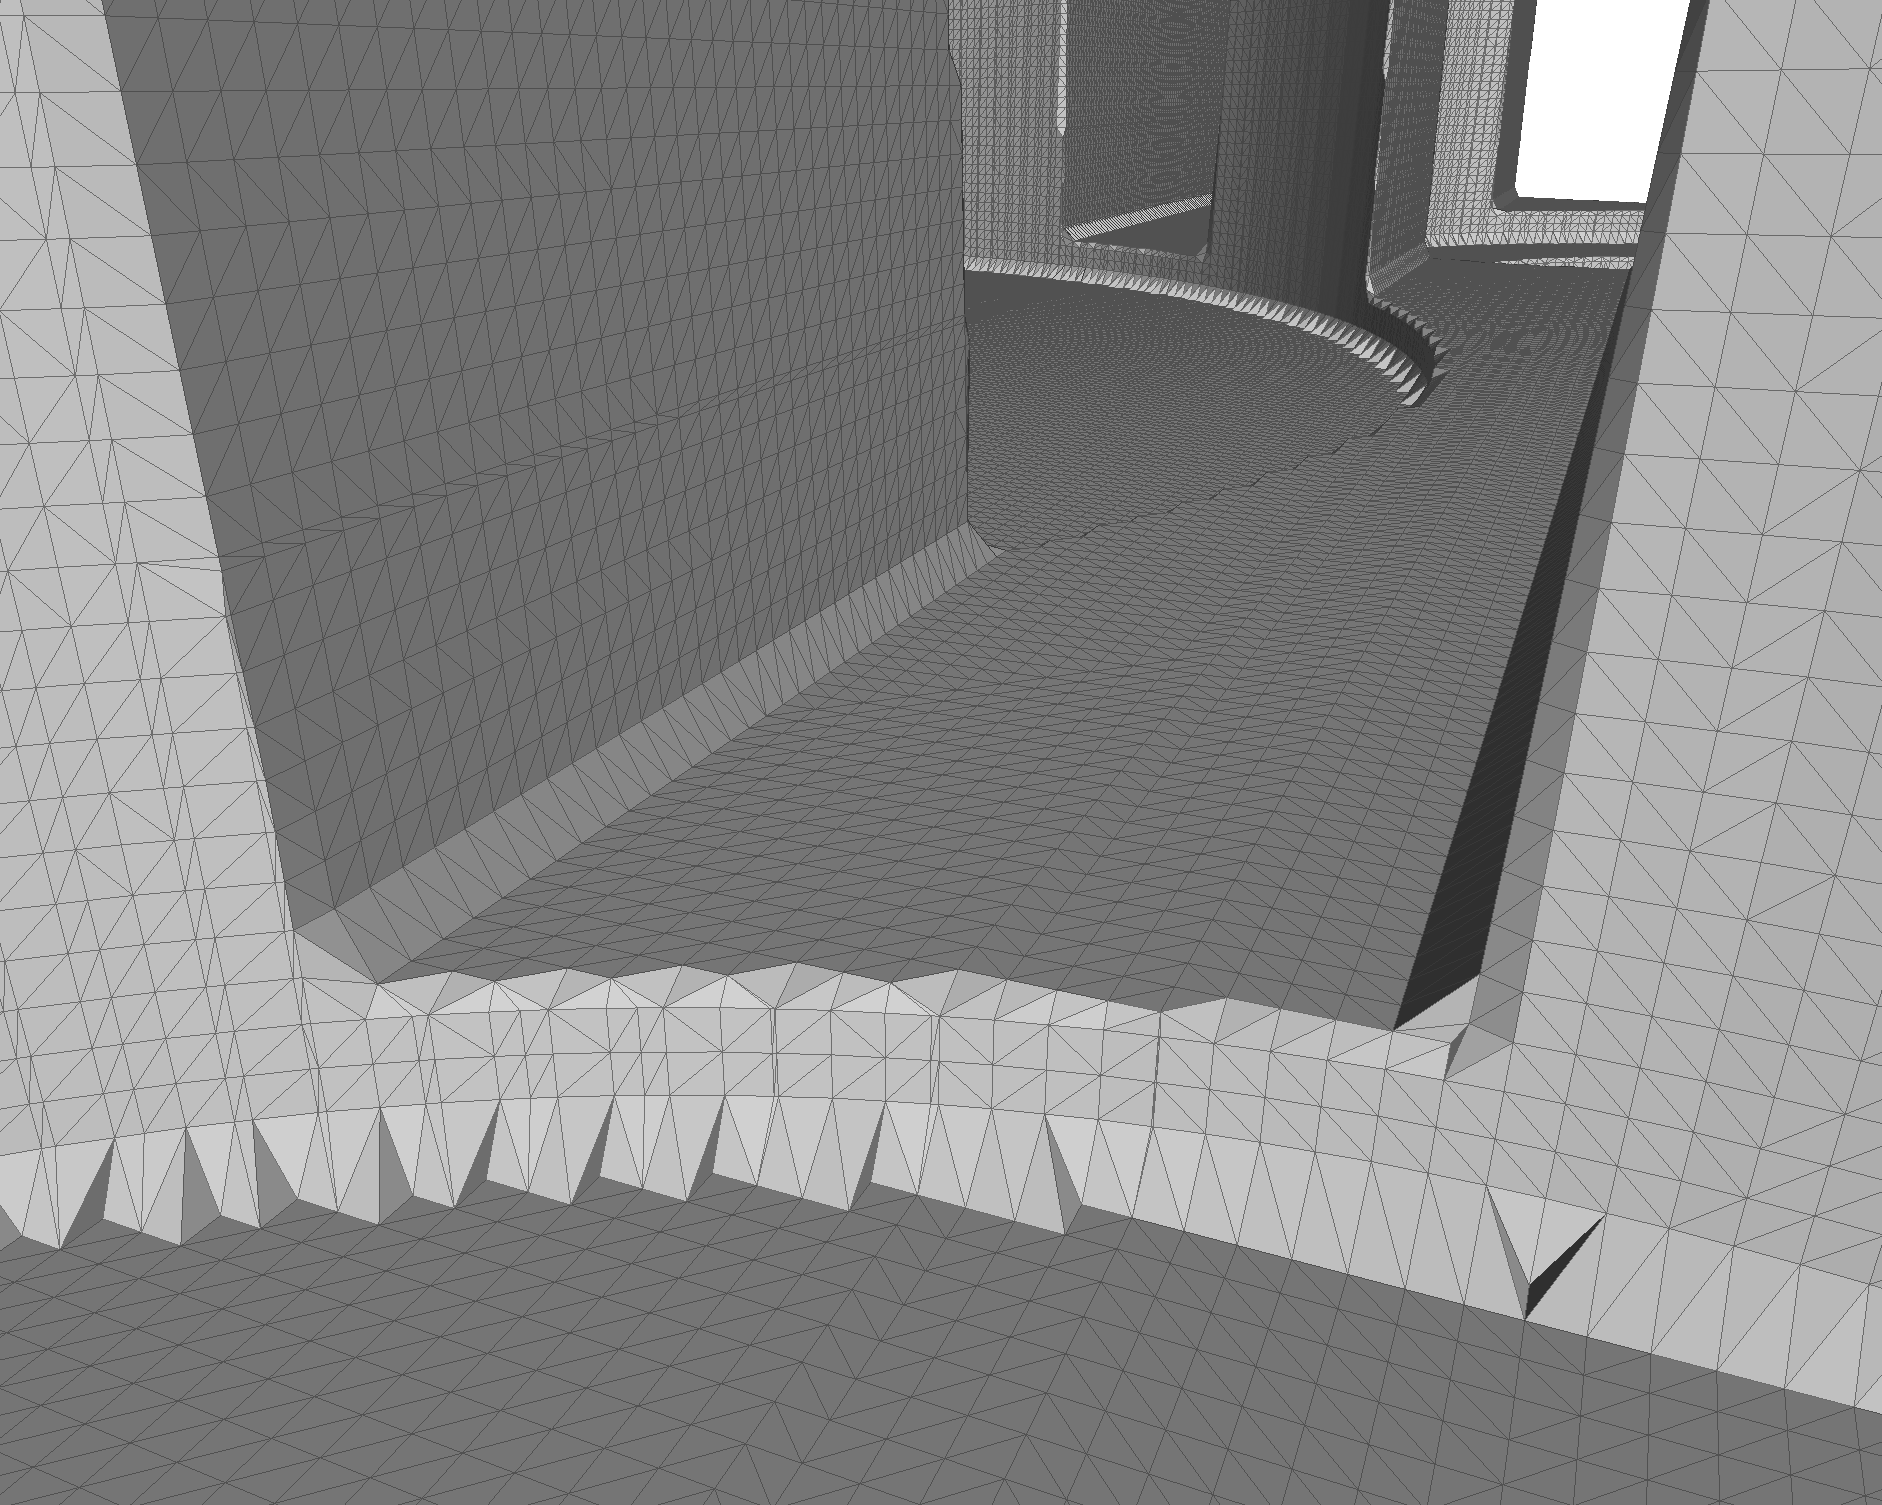
\includegraphics[width=\textwidth]{bpa_cylinder_head_edges}
		\caption{cylinder\_head edges}
		\label{fig:bpa_cylinder_head_edges}
	\end{subfigure}
	\begin{subfigure}[b]{0.49\textwidth}
		\centering
		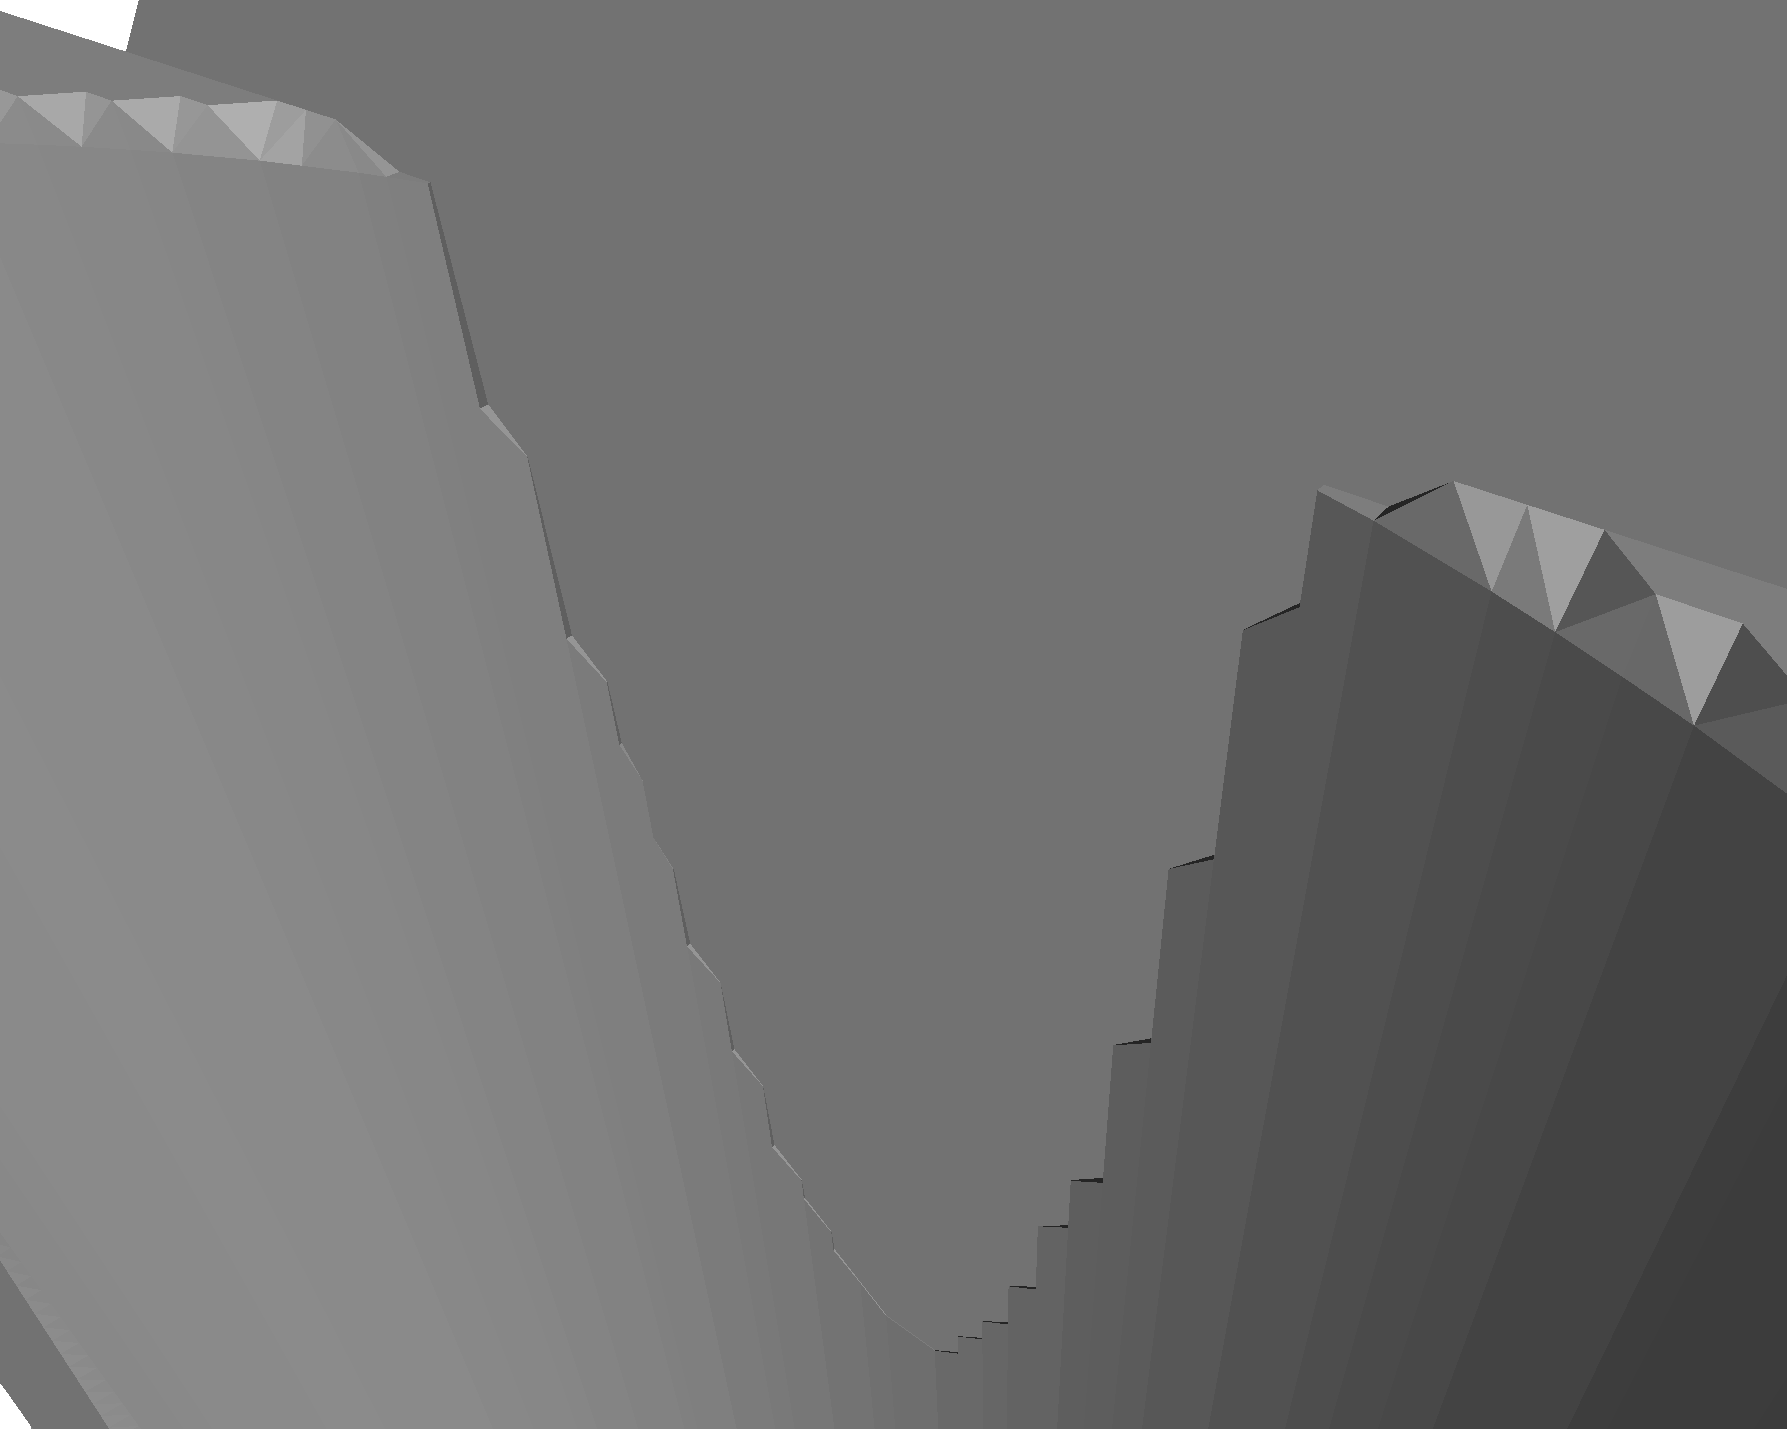
\includegraphics[width=\textwidth]{bpa_cylinder_head_thin_fin}
		\caption{cylinder\_head drilling at fin}
		\label{fig:bpa_cylinder_head_thin_fin}
	\end{subfigure}
	\caption{
		Details of the cylinder\_head scene rendered using MeshLab.
		The meshes have been extracted using the BPA approach with a resolution of 400.
	}
	\label{fig:bpa_cylinder_head_details}
\end{figure}
%
Concerning concave edges/features, the ball size is the BPA's limiting component as it does not allow the created surface to \enquote{crawl} into the sharp corners.
These features are simply rolled over.
Fine convex and concave features are only reconstructible from the normals of the point cloud and therefore ignored by the BPA.
Only geometry for which points are present in the point cloud is reconstructed by the BPA.
Surprisingly, due to the BPA's sole concentration on points, thin convex features such as the drilling at a fin of the cylinder\_head, \cf figure \ref{fig:bpa_cylinder_head_thin_fin}, are reconstructed quite robustly.
This part of the scene challenges the tri-dexel approach much more, as the cells almost collapse along one axis during slicing.

The turbine scene looks reasonable from a distance, \cf figure \ref{fig:bpa_turbine}.
However, the BPA has a hard time reconstructing the concave grooves, failing horribly at lower resolutions.
Figure \ref{fig:bpa_grooves} shows the turbine's grooves reconstructed from point clouds with various resolutions.
%
\begin{figure}
	\centering
	\begin{subfigure}[b]{0.24\textwidth}
		\centering
		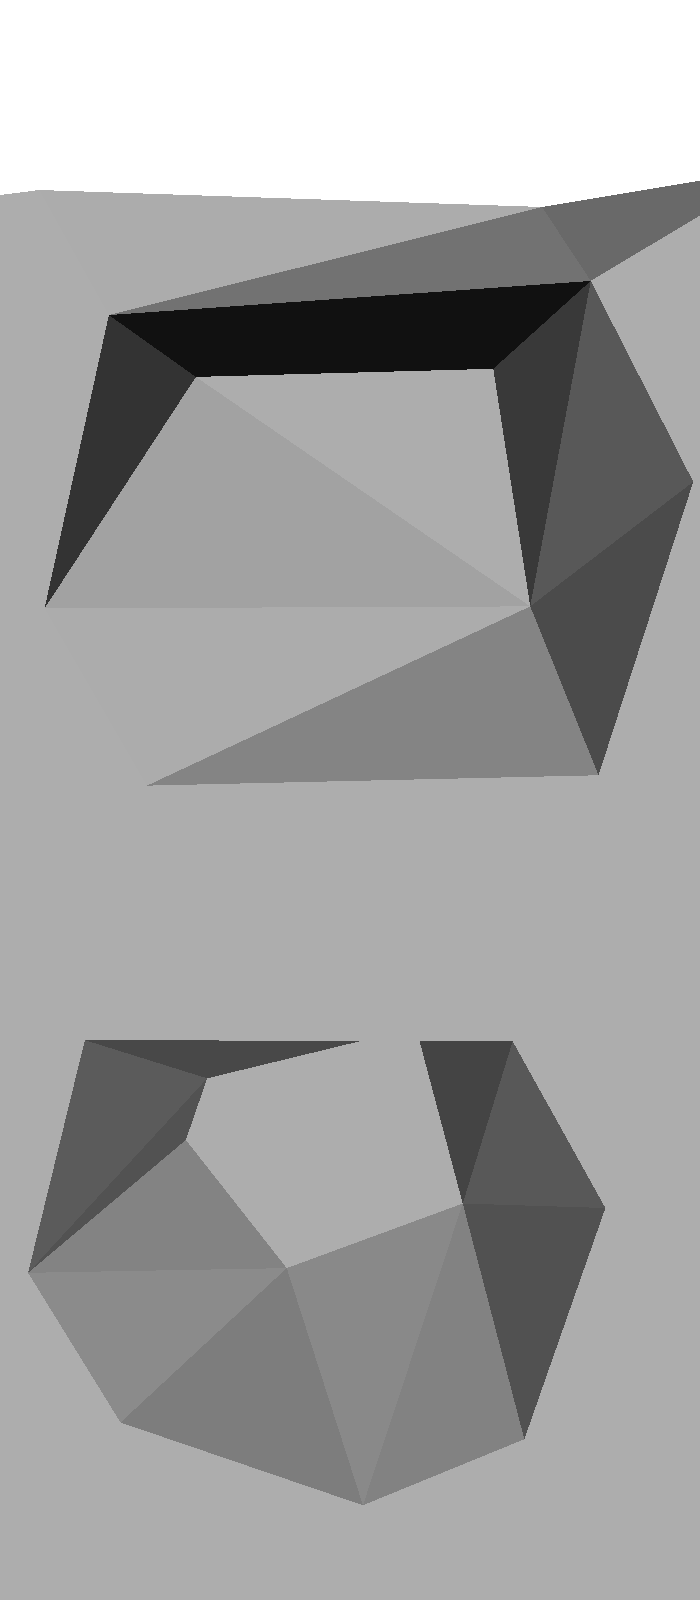
\includegraphics[width=\textwidth]{bpa_turbine_groove_50}
		\caption{50}
		\label{fig:bpa_turbine_groove_50}
	\end{subfigure}
	\begin{subfigure}[b]{0.24\textwidth}
		\centering
		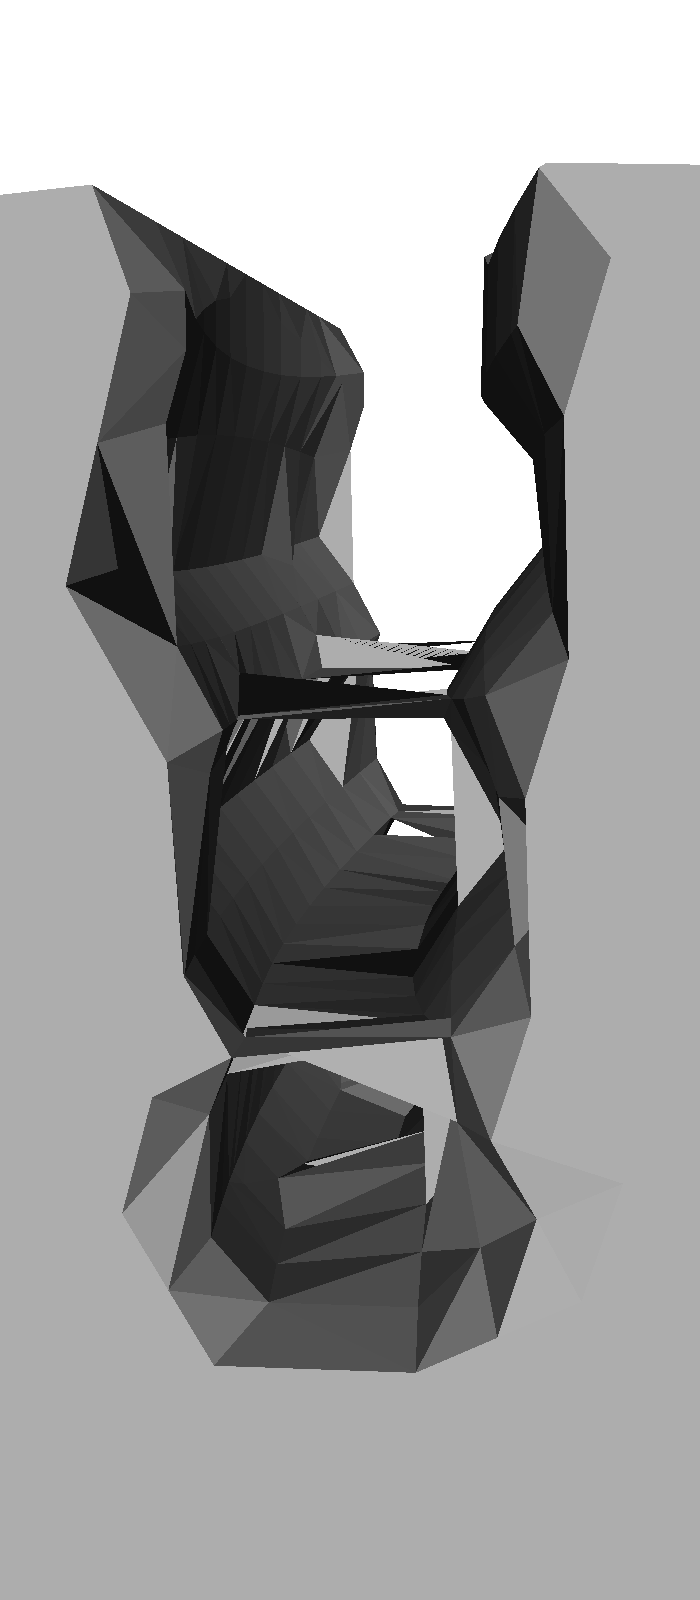
\includegraphics[width=\textwidth]{bpa_turbine_groove_100}
		\caption{100}
		\label{fig:bpa_turbine_groove_100}
	\end{subfigure}
	\begin{subfigure}[b]{0.24\textwidth}
		\centering
		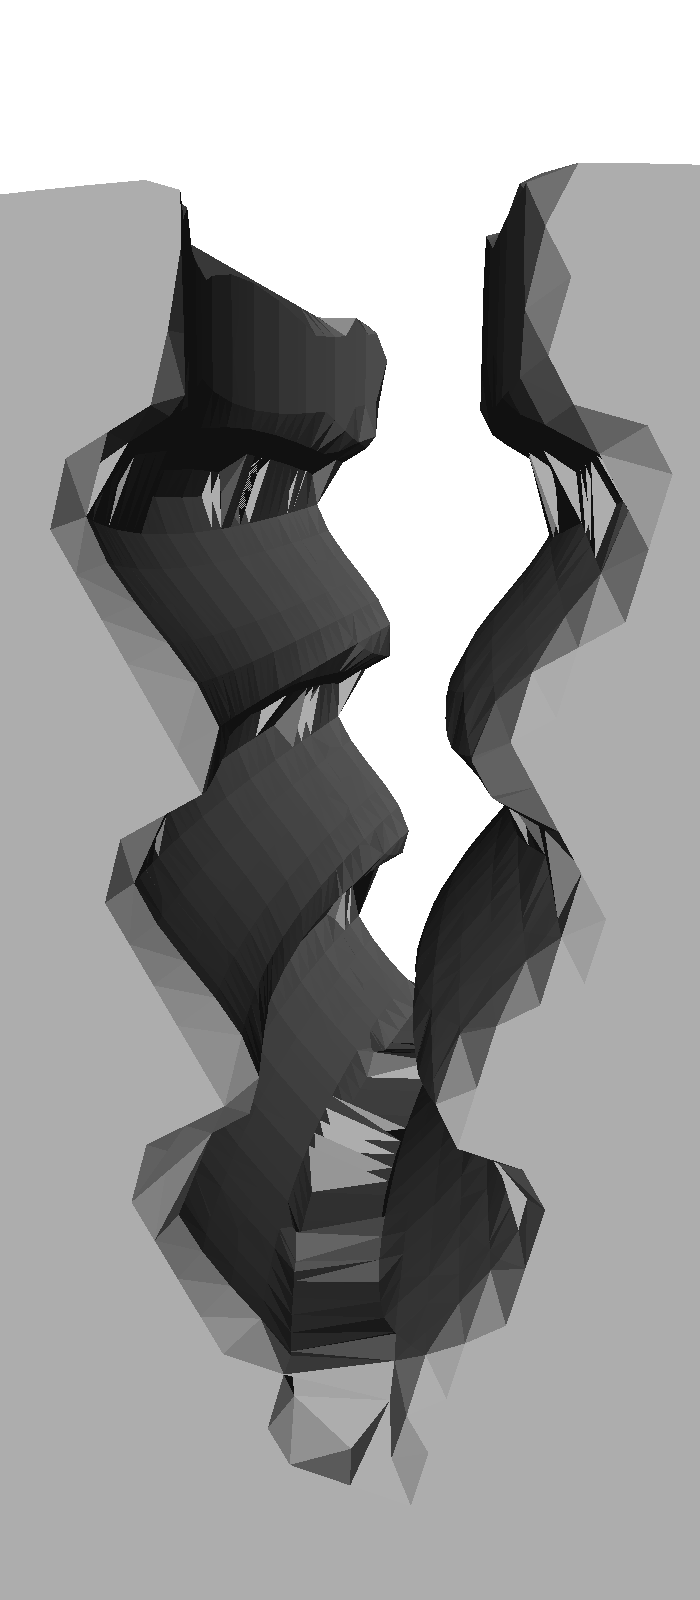
\includegraphics[width=\textwidth]{bpa_turbine_groove_200}
		\caption{200}
		\label{fig:bpa_turbine_groove_200}
	\end{subfigure}
	\begin{subfigure}[b]{0.24\textwidth}
		\centering
		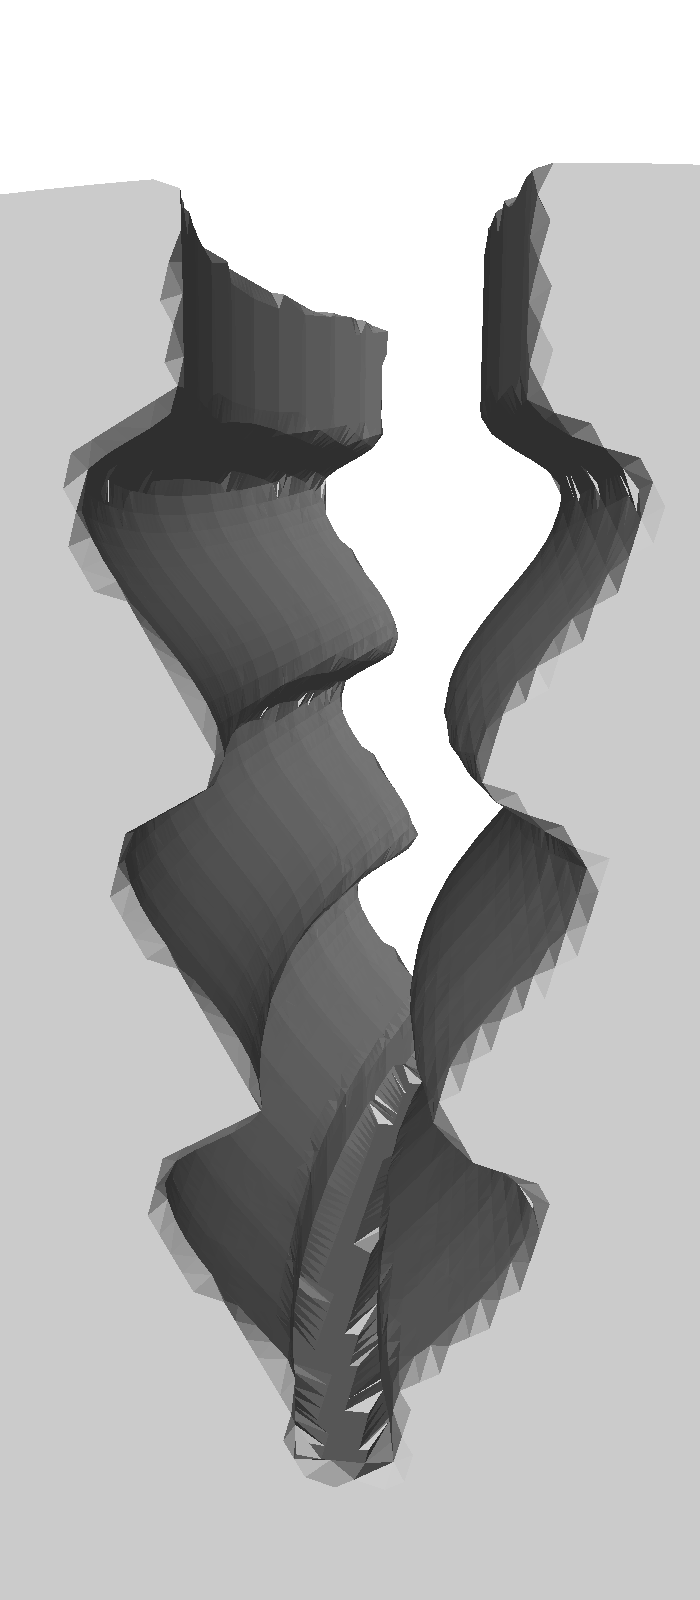
\includegraphics[width=\textwidth]{bpa_turbine_groove_400}
		\caption{400}
		\label{fig:bpa_turbine_groove_400}
	\end{subfigure}
	\caption{
		Detailed renderings with the same perspective of a groove of the turbine scene using MeshLab.
		The meshes were created using the BPA reconstruction algorithm run on a point cloud with the resolutions 50, 100, 200 and 400.
	}
	\label{fig:bpa_grooves}
\end{figure}
%
At a resolution of 50, the grooves are simply too small for the ball to roll inside.
Compared with the tri-dexel approach using the same resolution, which succeeds in recreating the groove, the BPA's result is terrible.
Increasing the resolution to 100 allows the ball to slip inside the groove, although still a lot of geometry is created spanning it.
At a resolution of 200, the groove becomes clearly visible.
However, the concave indentations at the groove's sides are still captured badly, especially the indentation at the bottom.
Finally, at a resolution of 400 the groove is reconstructed almost correctly, which only a few artifacts at the bottom.
Compared again with the tri-dexel results for the turbine's grooves, \cf figure \ref{fig:td_grooves}, the BPA requires approximately twice the resolution for a similar visual quality.

A further problem of the BPA is its instability inside concave features which are slightly larger than the ball as well as the possibility of the ball to roll inside the point cloud.
Figure \ref{fig:bpa_issues} shows cases for these two problems.%
\begin{figure}
	\centering
	\begin{subfigure}[b]{0.49\textwidth}
		\centering
		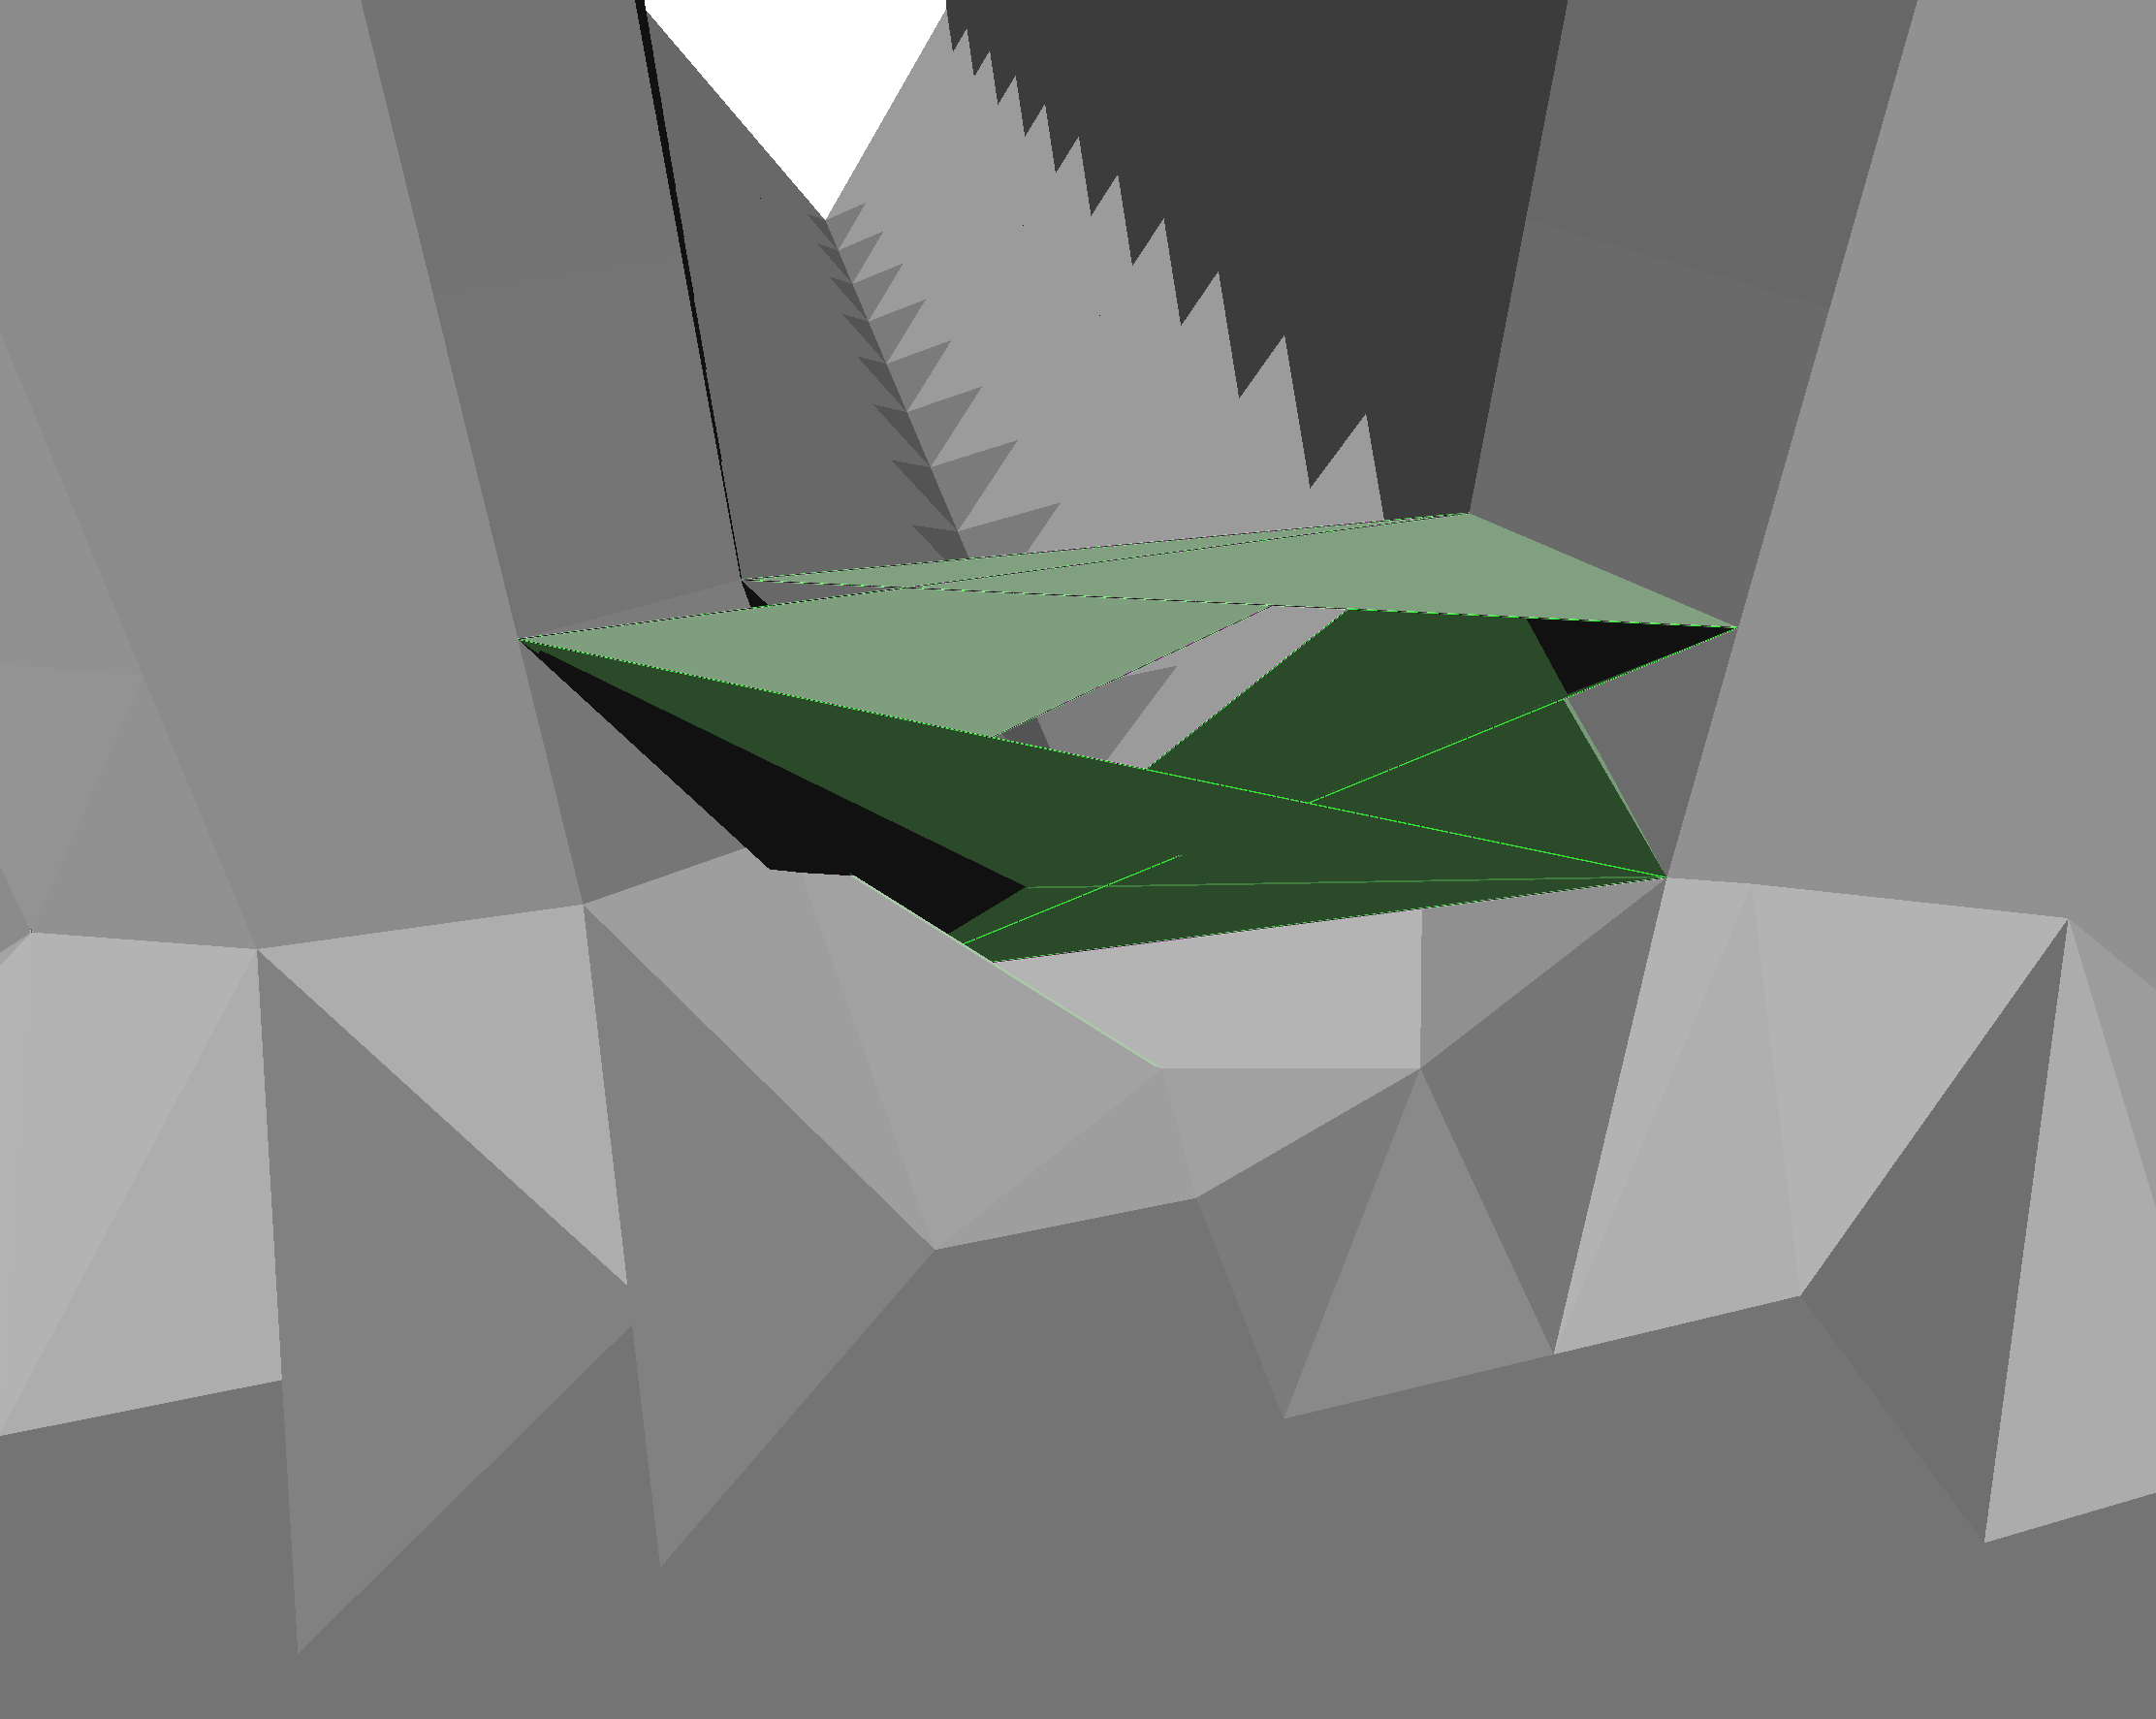
\includegraphics[width=\textwidth]{bpa_cylinder_head_non_manif}
		\caption{cylinder\_head 50}
		\label{fig:bpa_cylinder_head_non_manif}
	\end{subfigure}
	\begin{subfigure}[b]{0.49\textwidth}
		\centering
		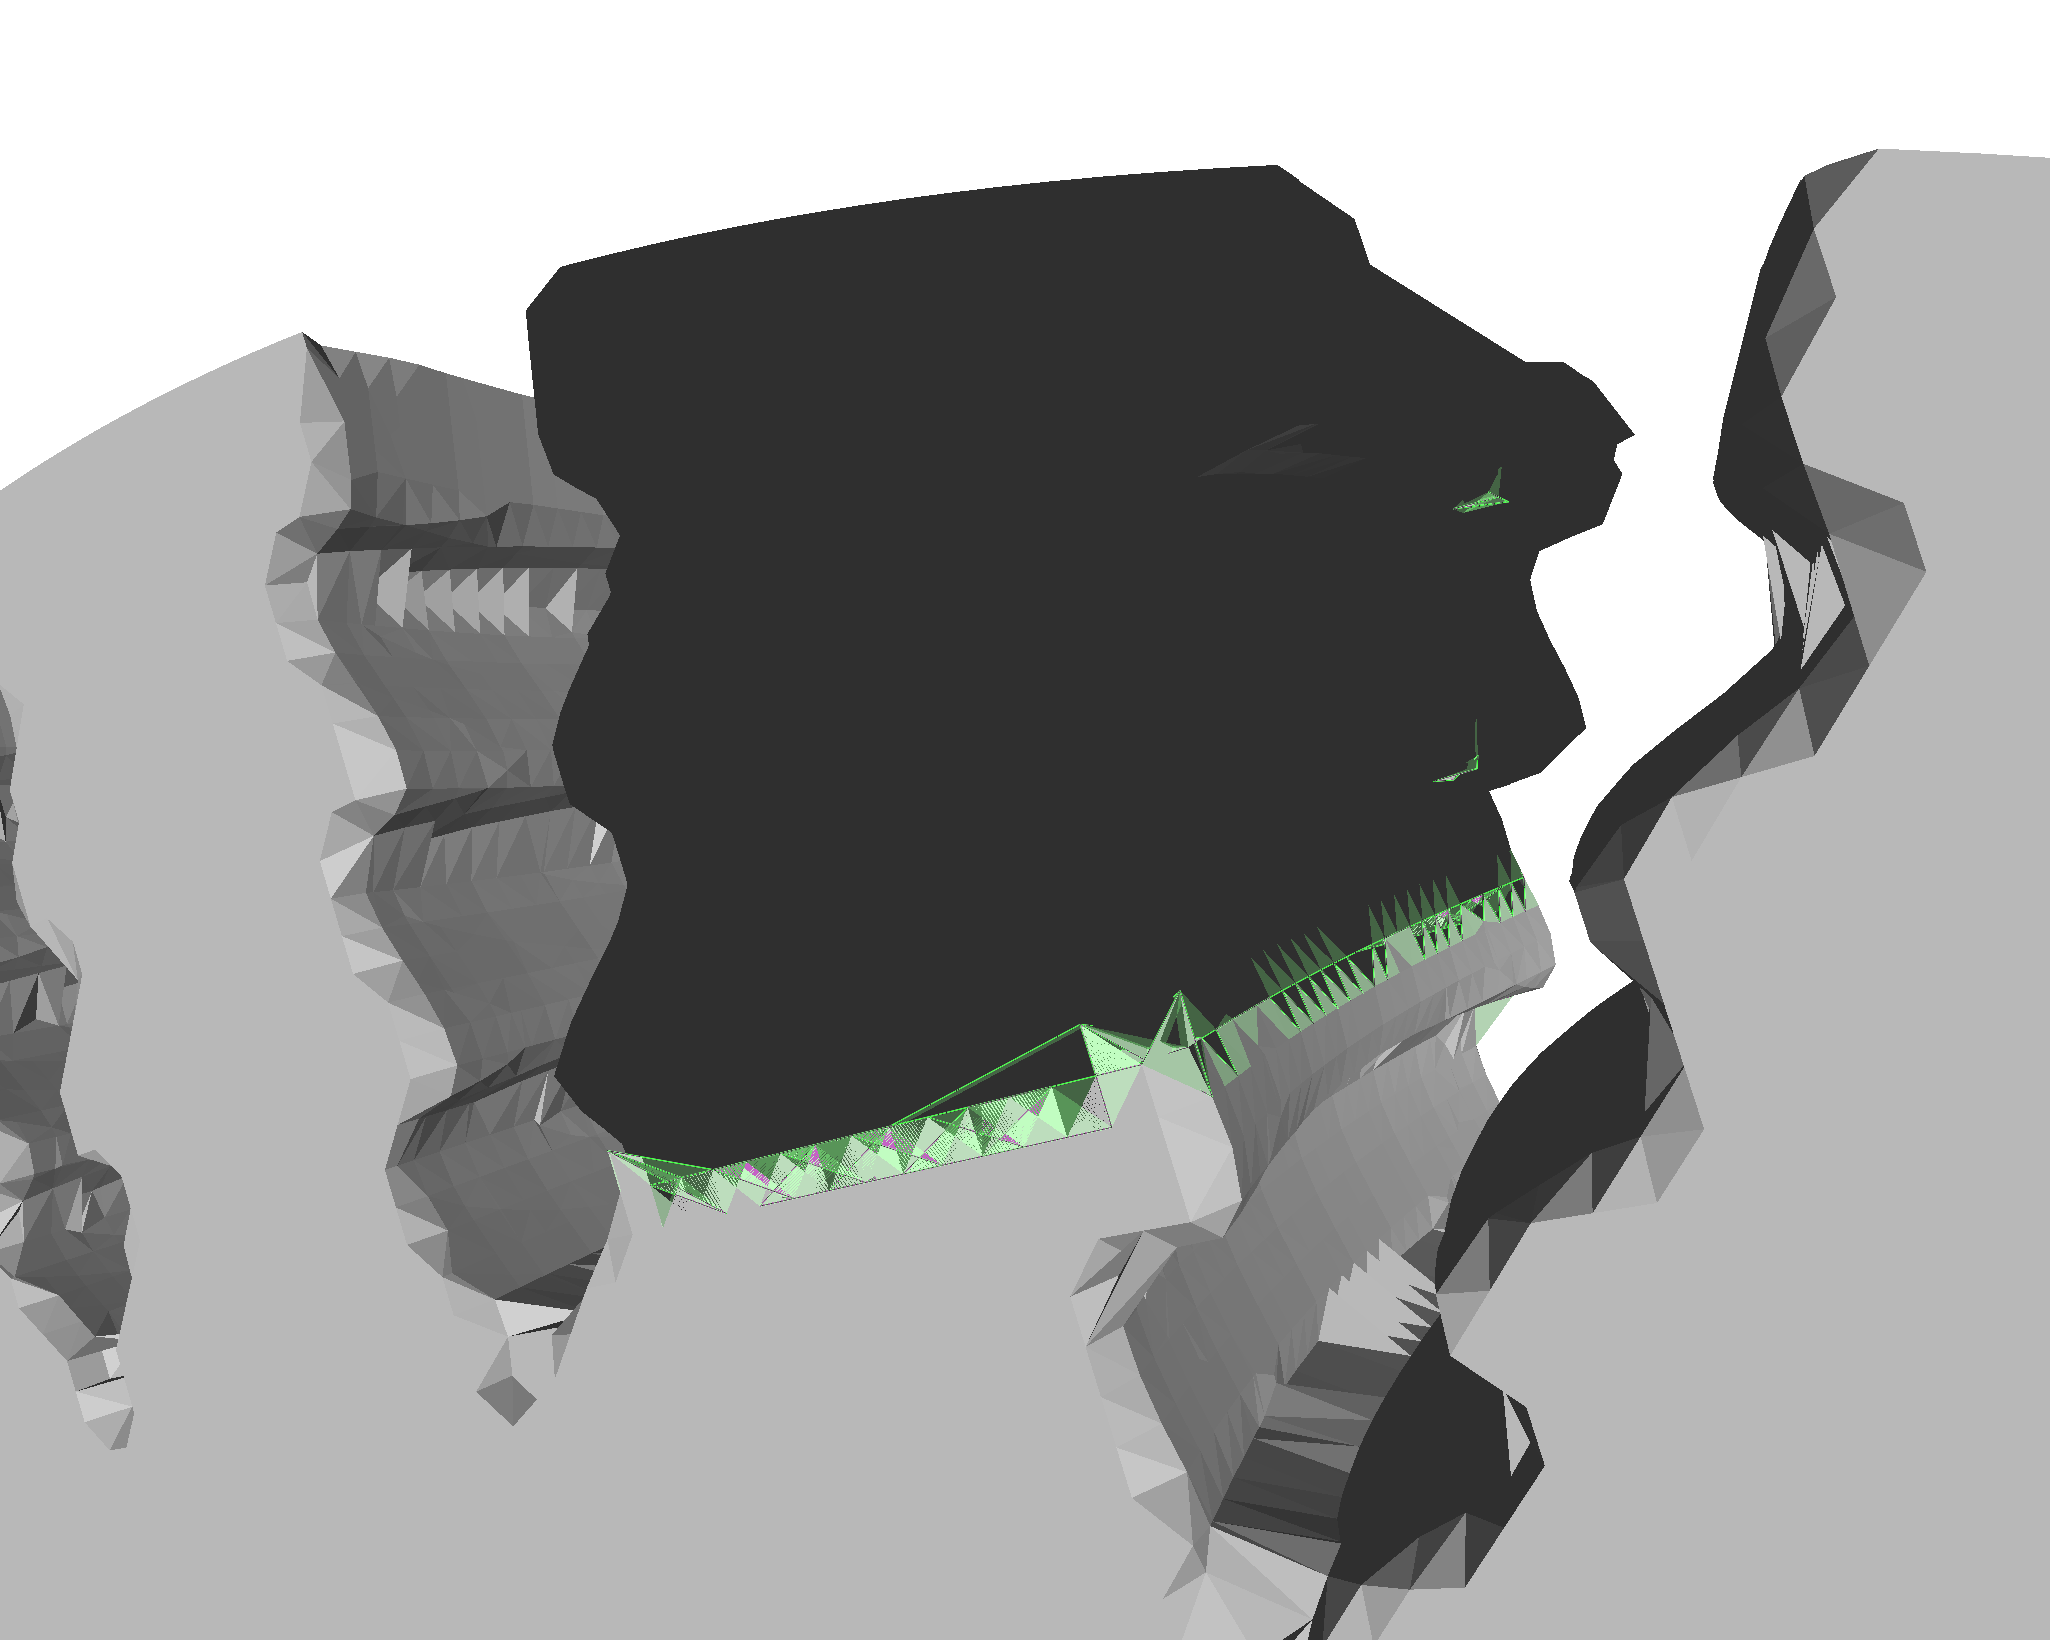
\includegraphics[width=\textwidth]{bpa_turbine_inside}
		\caption{turbine 200}
		\label{fig:bpa_turbine_inside}
	\end{subfigure}
	\caption{
		Error in the cylinder\_head and turbine scene after BPA reconstruction, rendered using MeshLab.
		Boundary edges are marked in green.
	}
	\label{fig:bpa_issues}
\end{figure}

The left rendering, figure \ref{fig:bpa_cylinder_head_non_manif}, shows the creation of holes and non-manifold triangles between two fins of the cylinder\_head.
Such problems occur if the ball suddenly switches sides inside a concave feature, creating a triangle spanning the indentation.
Usually, the edges of these triangles cannot be pivoted further and remain boundaries.

The right rendering shows a cog of the turbine where the ball has fell inside the point cloud.
Between the differently oriented meshes, one created from outside, one from inside, lots of boundary edges and overlapping triangles are created.
If sufficient density of the point cloud is guaranteed, this case should, theoretically, never occur.
However, since all pivotings are subject to numeric calculations, there are indeed cases where the ball may still roll inside the point cloud.
Increasing the ball's size may help to minimize the likelihood of such an error, but comes at the cost of worse feature reconstruction.

Concerning the created boundary edges and holes, \cf table \ref{tbl:bpa_boundary edges}, the BPA is quite robust if the point cloud does not contain concave features which are slightly larger than the size of the ball.
%
\begin{table}
	\centering
	\begin{tabular}{l|r|r|r|r}
		resolution     &  50 &  100 &  200 &  400 \\
		\midrule
		cube2          &   0 &    0 &    0 &    0 \\
		cylinders\_d   &   0 &    0 &    0 &    0 \\
		cylinders      &   0 &    0 &    0 &    0 \\
		cylinder\_head & 110 &    0 &    0 &    0 \\
		impeller       &   0 &    0 &    0 &    0 \\
		impeller\_2    &   0 &    0 &    0 &    0 \\
		turbine        &   0 & 3055 & 1721 & 3293 \\
	\end{tabular}
	\caption{
		Created boundary edges by the BPA surface extraction.
		All values were measured using MeshLab.
	}
	\label{tbl:bpa_boundary edges}
\end{table}
%
The only point clouds where boundary edges have been generated are the cylinder\_head, at a resolution of 50, and all turbine clouds higher than 50.

In all of these cases, the ball rolls inside a concave feature/hole and creates triangles spanning the sides of the feature, \cf figure \ref{fig:bpa_cylinder_head_non_manif} and \ref{fig:bpa_turbine_groove_100}.
These cases could be resolved by analyzing the created mesh, finding non-manifold vertices/edges, removing affected triangles and rerunning the BPA on the remaining holes, maybe with different ball sizes.
If sufficient memory is available, the point cloud resolution may also be increased which allows the ball to be smaller and have more space to pivot in such small features.

In the turbine cases, the ball also frequently rolls inside the point cloud, even if it is only for smaller regions.
At the border of these regions, the mesh orientation changes and usually causes boundary edges to be left, as the BPA is not allowed to attach new triangles to existing triangles if they are differently orientated.
This kind of problem occurs primarily numerically and may only be mitigated by implementing further checks into the pivoting code.


Finally, to show the suitability of the point cloud for other algorithms outside the VML, a few renderings of the more complex scenes from meshes reconstructed with the Poisson reconstruction approach are discussed.
Figure \ref{fig:poisson_results} shows renderings of the cylinder\_head and impeller scene after applying the Poisson surface reconstruction filter available in MeshLab.
%
\begin{figure}
	\centering
	\begin{subfigure}[b]{0.49\textwidth}
		\centering
		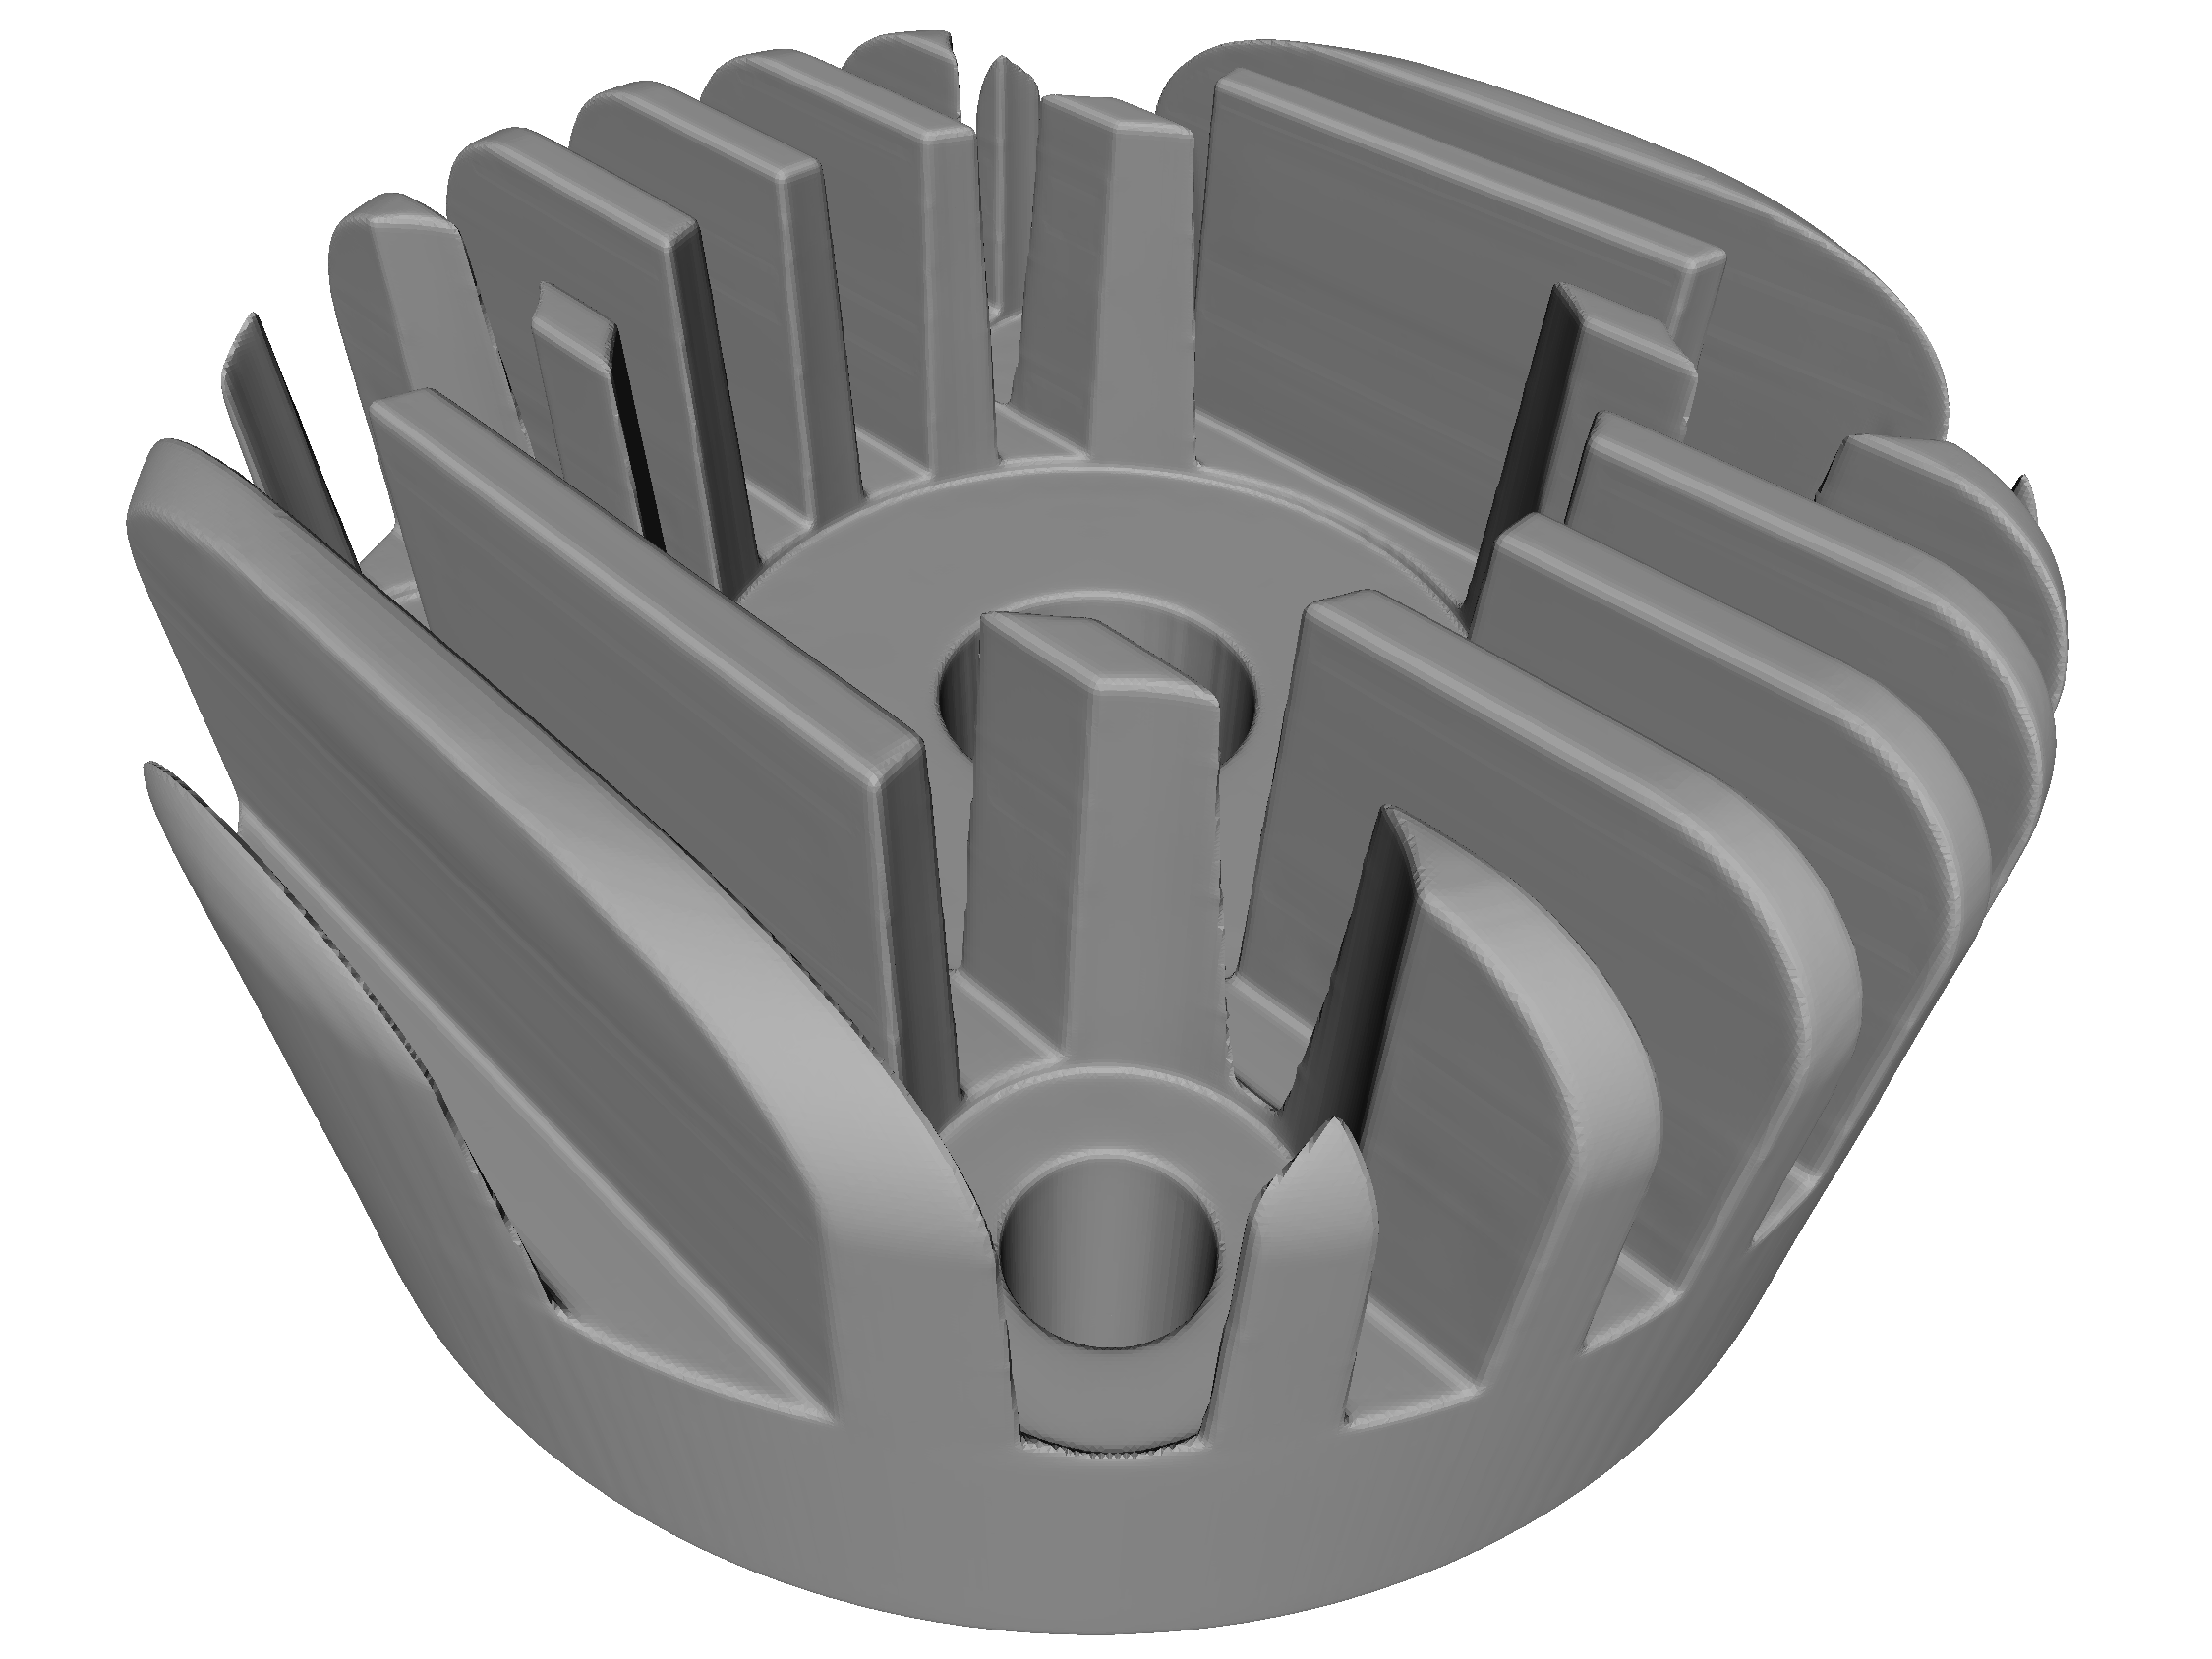
\includegraphics[width=\textwidth]{poi_cylinder_head}
		\caption{cylinder\_head}
		\label{fig:poi_cylinder_head}
	\end{subfigure}
	\begin{subfigure}[b]{0.49\textwidth}
		\centering
		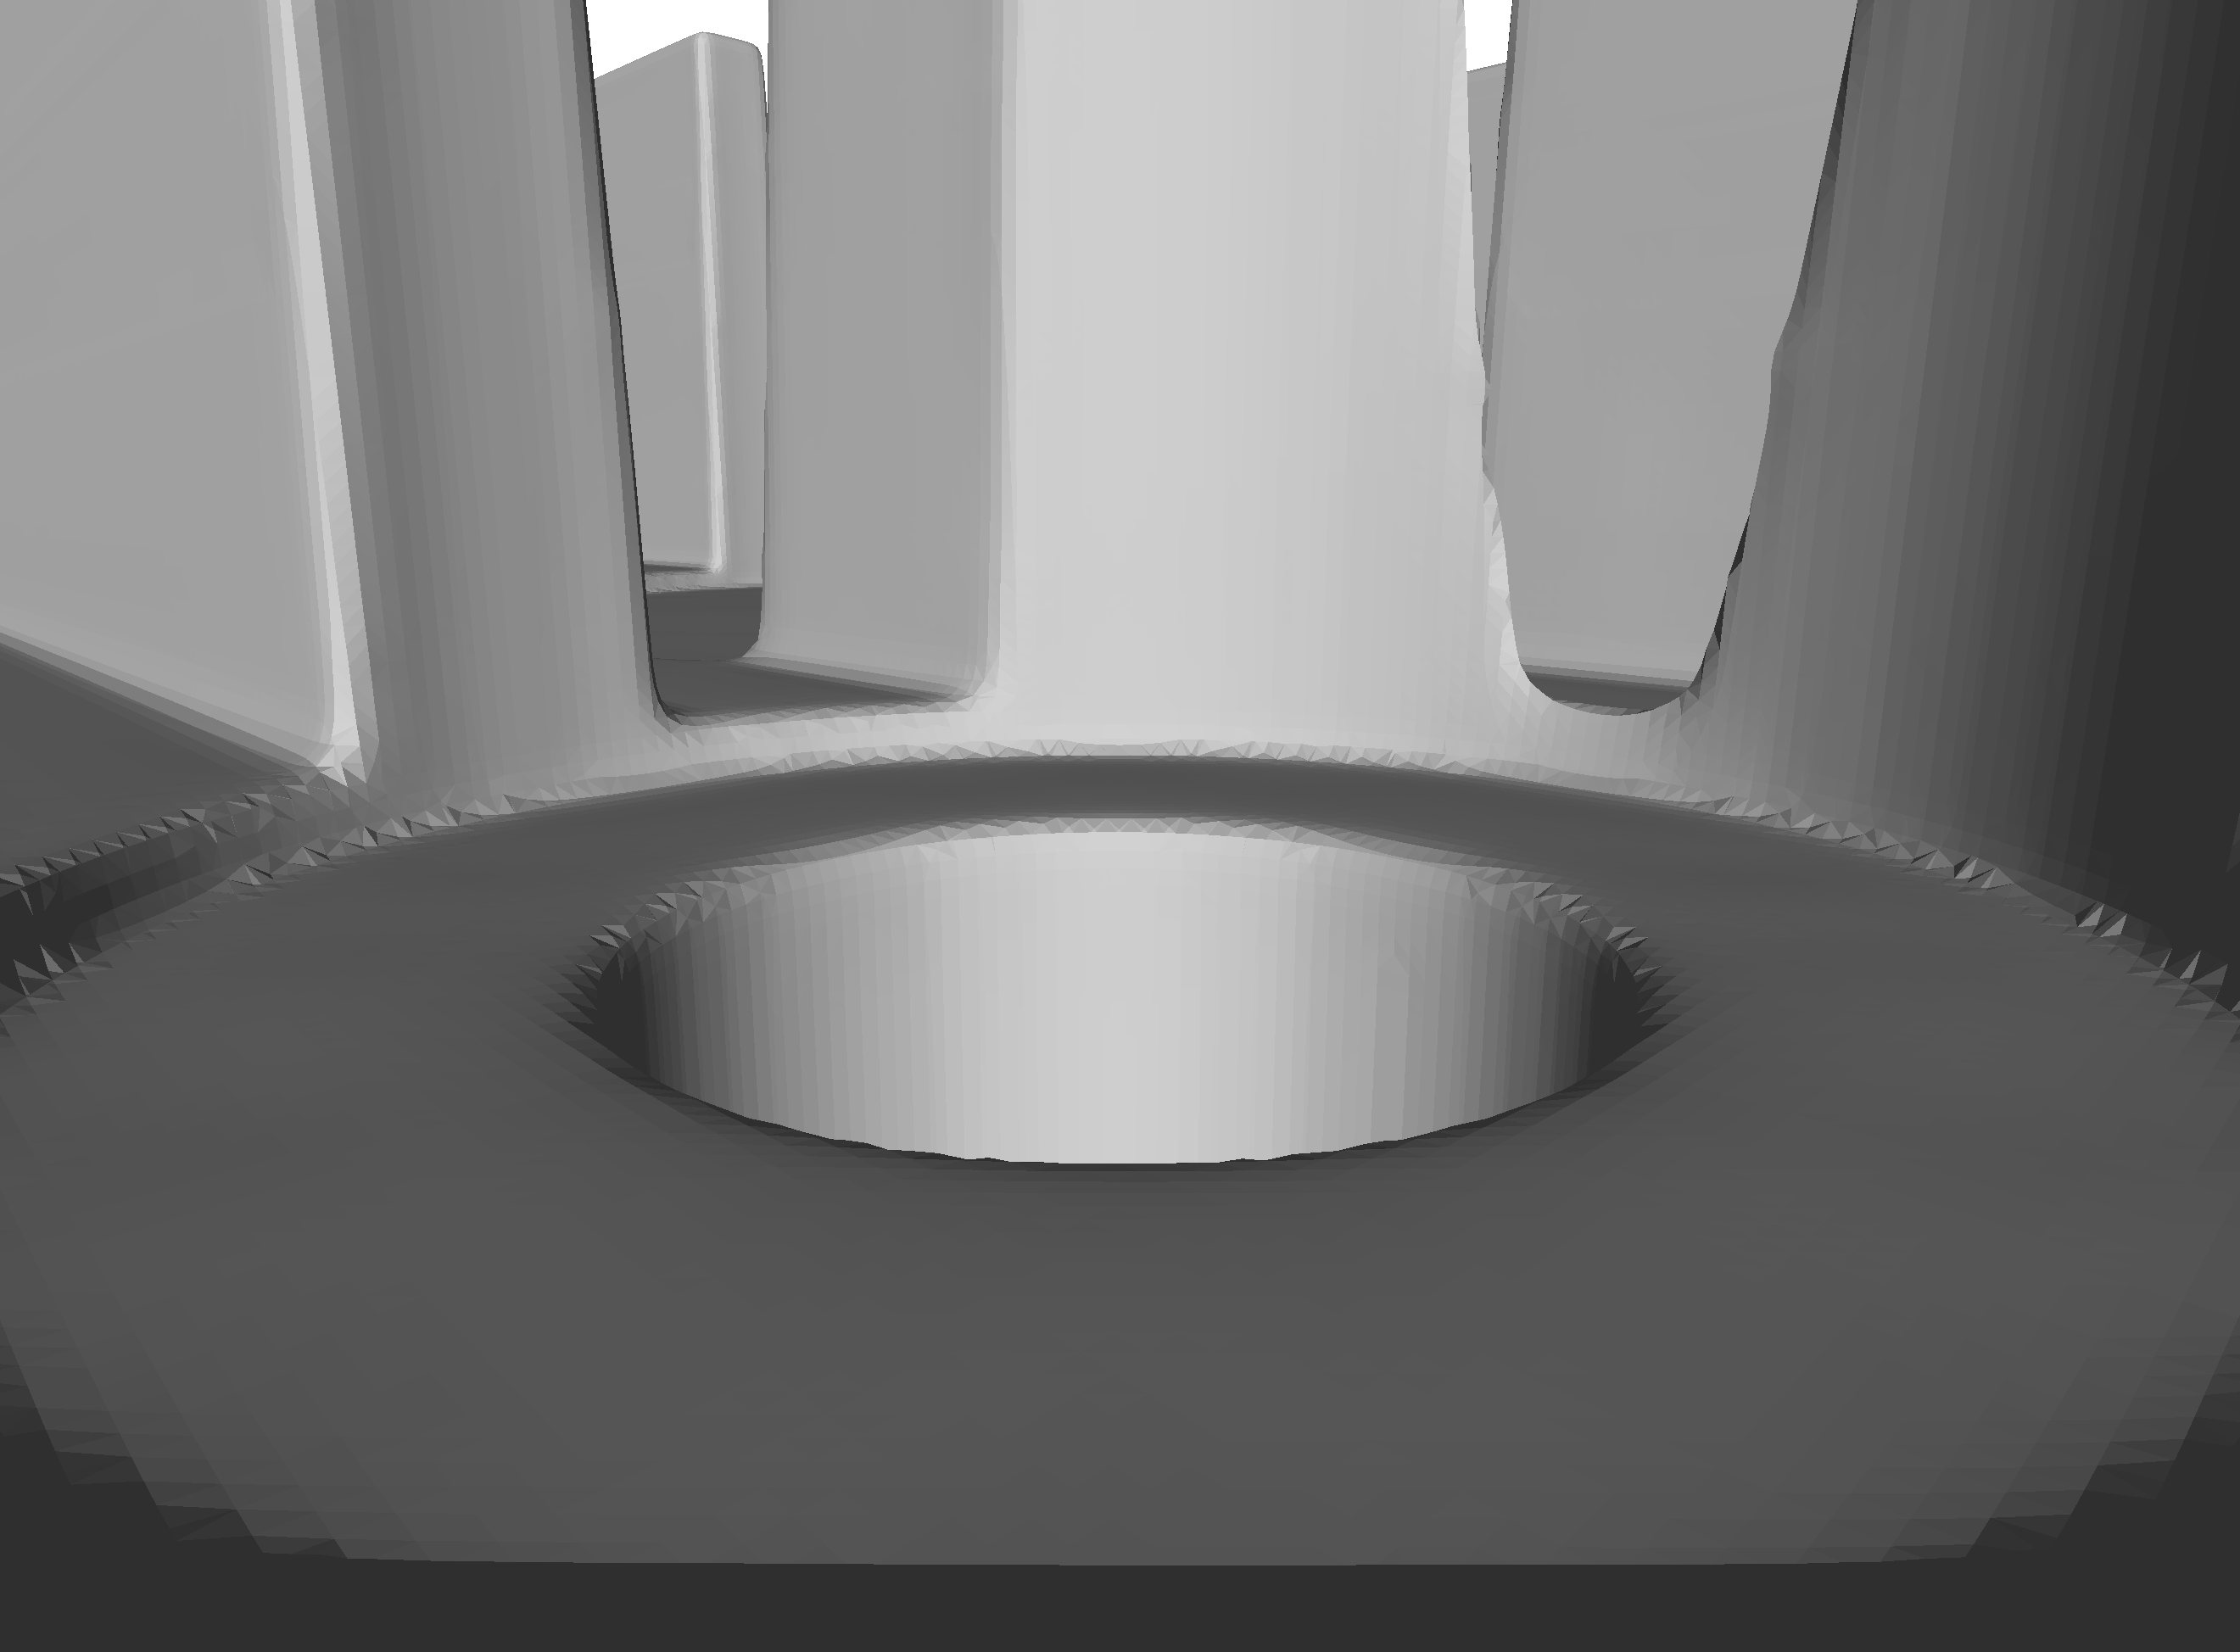
\includegraphics[width=\textwidth]{poi_cylinder_head_detail}
		\caption{cylinder\_head details}
		\label{fig:poi_cylinder_head_detail}
	\end{subfigure}
	\begin{subfigure}[b]{0.49\textwidth}
		\centering
		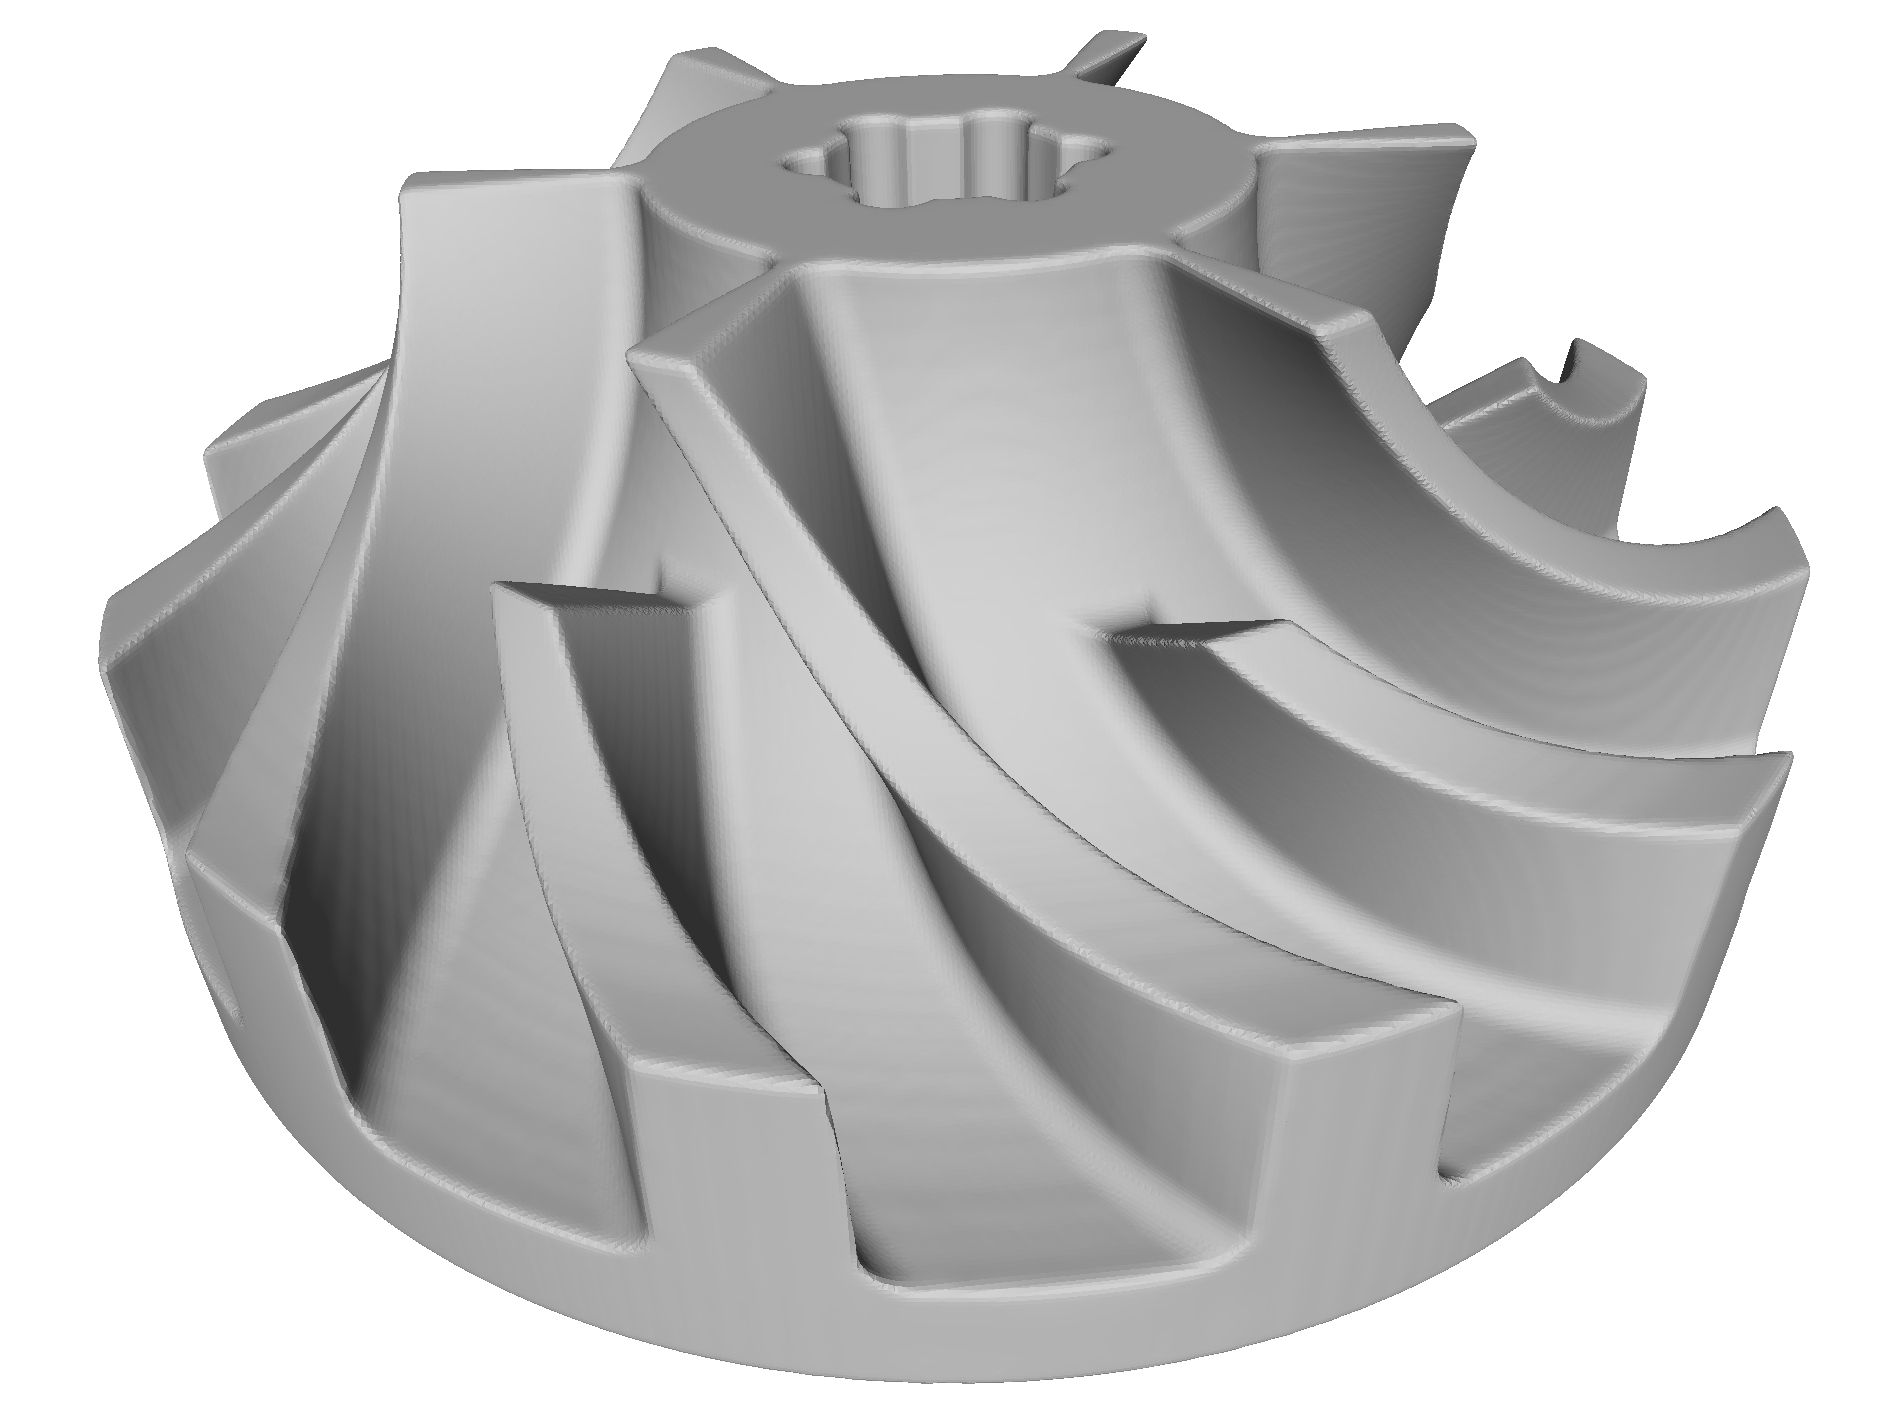
\includegraphics[width=\textwidth]{poi_hq_impeller}
		\caption{impeller}
		\label{fig:poi_hq_impeller}
	\end{subfigure}
	\begin{subfigure}[b]{0.49\textwidth}
		\centering
		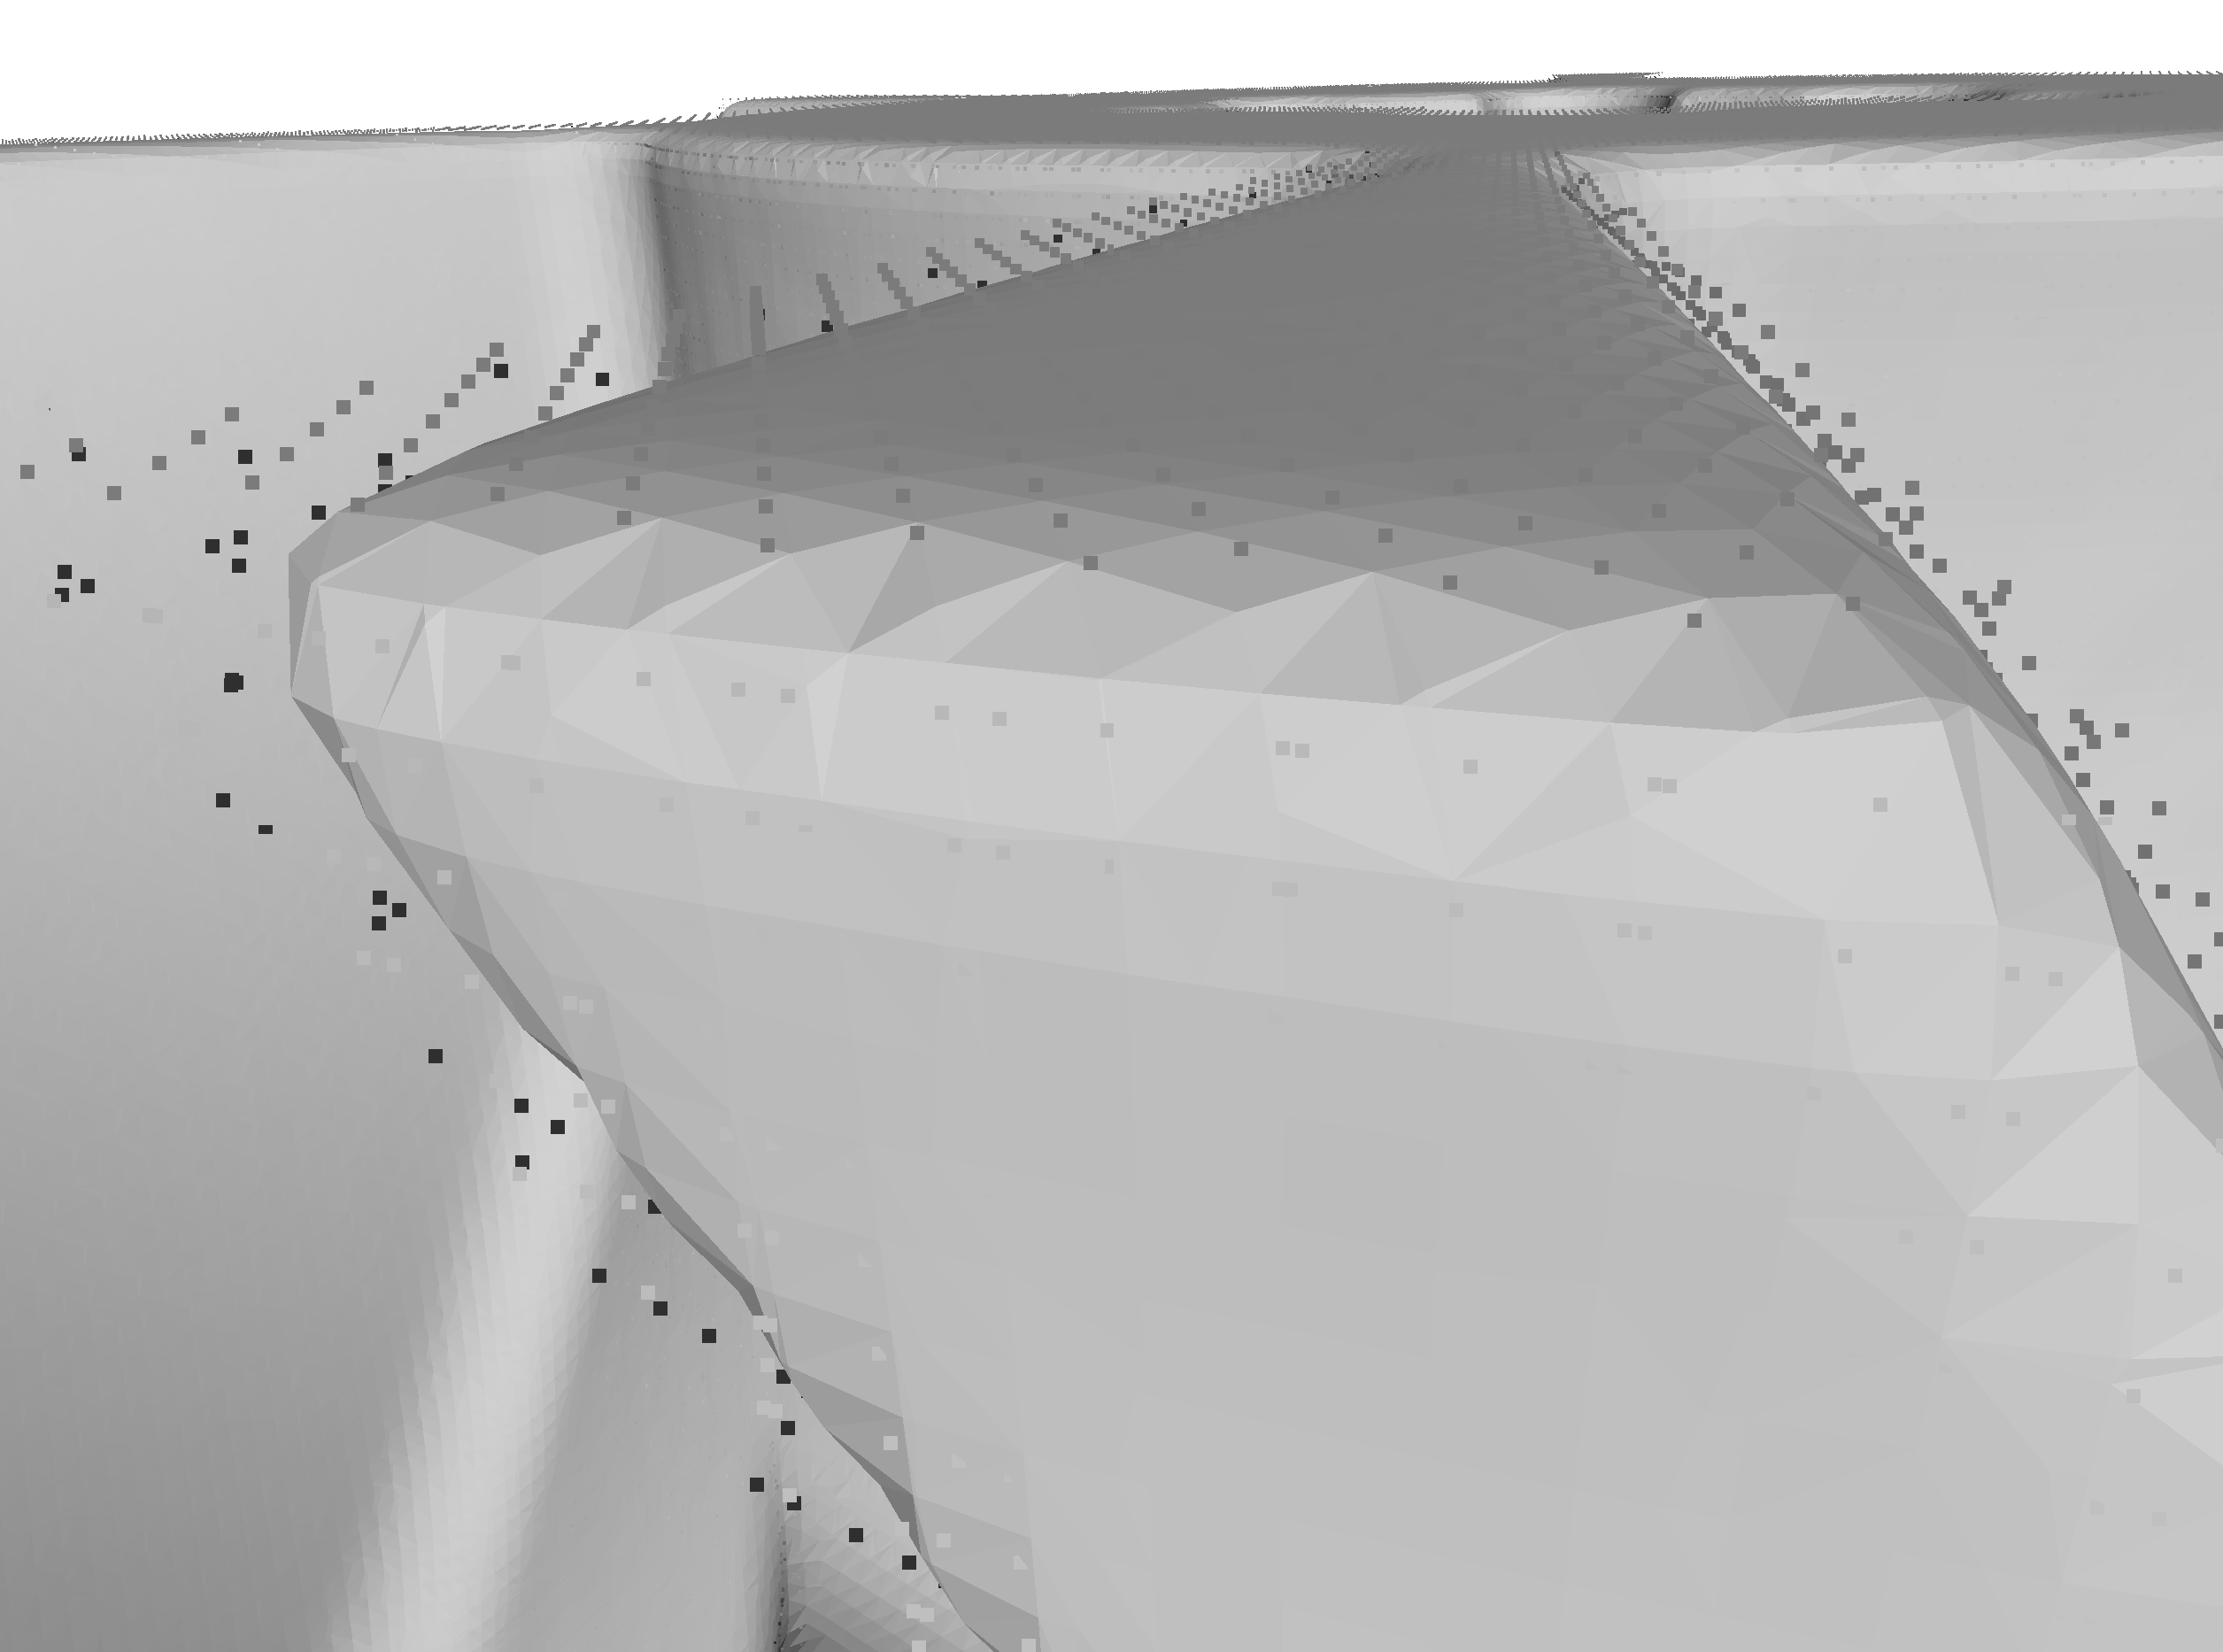
\includegraphics[width=\textwidth]{poi_hq_impeller_points}
		\caption{impeller edges}
		\label{fig:poi_hq_impeller_points}
	\end{subfigure}
	\caption{
		Renderings of the cylinder\_head and impeller scenes of reconstructions using the Poisson surface reconstruction filter from MeshLab.
		The point cloud was created with a resolution of 400.
		The Poisson filter was parameterized with an octree depth of 10, solver divide at 8, 1 sample per node and a surface offsetting of 1, \cf corresponding dialog in MeshLab.
	}
	\label{fig:poisson_results}
\end{figure}
%
As the Poisson algorithm tries to be robust against inhomogeneous and noisy inputs, sharp features are considered outliers and lost during the function fitting process.
This gives the reconstructed meshes a smooth and roundish appearance, as visible in the general renderings in figures \ref{fig:poi_cylinder_head} and \ref{fig:poi_hq_impeller}.
The detailed rendering of a drilling of the cylinder\_head in figure \ref{fig:poi_cylinder_head_detail} further demonstrates the loss of sharp edges.
Additionally, the structure in the upper right, the drilling at the fin, is almost completely lost as the structure is too thin to allow the creation of a surface.

Figure \ref{fig:poi_hq_impeller_points} shows a reconstructed blade of the impeller together with the sampled point cloud.
The amount of lost volume, especially at the blade's tip and edge at the left, is clearly visible, as the surface only bends towards the points in flatter regions.
Nevertheless, the resulting triangulation is appealing with even a bit of adaptivity, containing larger triangles in flatter regions.
All runs of the algorithm generated manifold and closed meshes for all tested point clouds.

Figure \ref{fig:poi_grooves} shows a groove of the turbine reconstructed from point clouds with various resolutions.
%
\begin{figure}
	\begin{subfigure}[b]{0.24\textwidth}
		\centering
		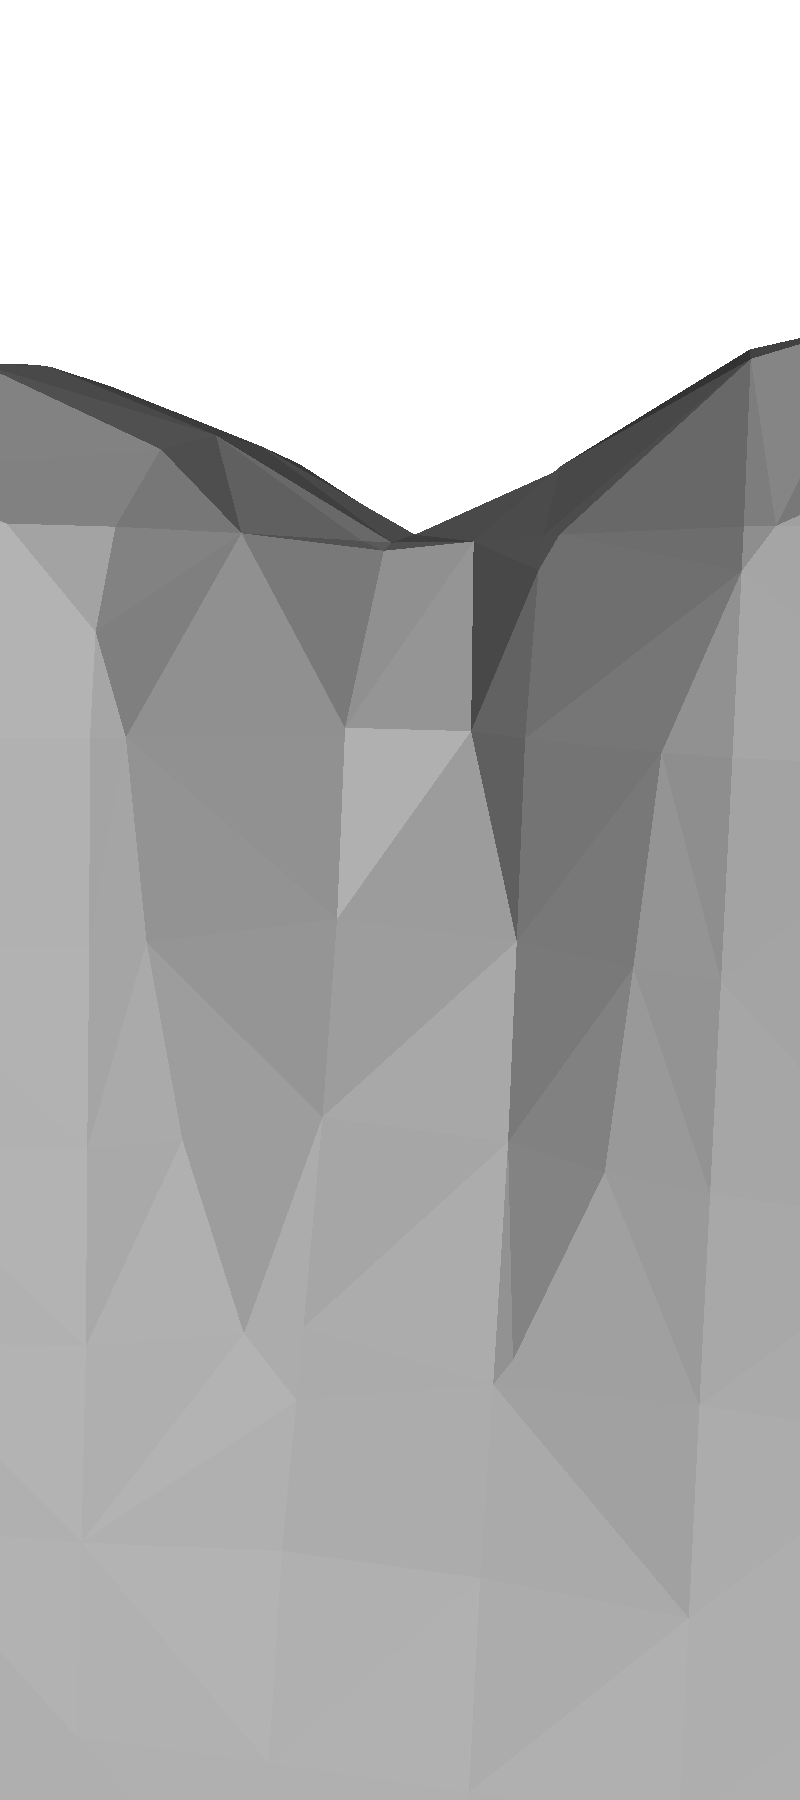
\includegraphics[width=\textwidth]{poi_turbine_groove_50}
		\caption{50}
		\label{fig:poi_turbine_groove_50}
	\end{subfigure}
	\begin{subfigure}[b]{0.24\textwidth}
		\centering
		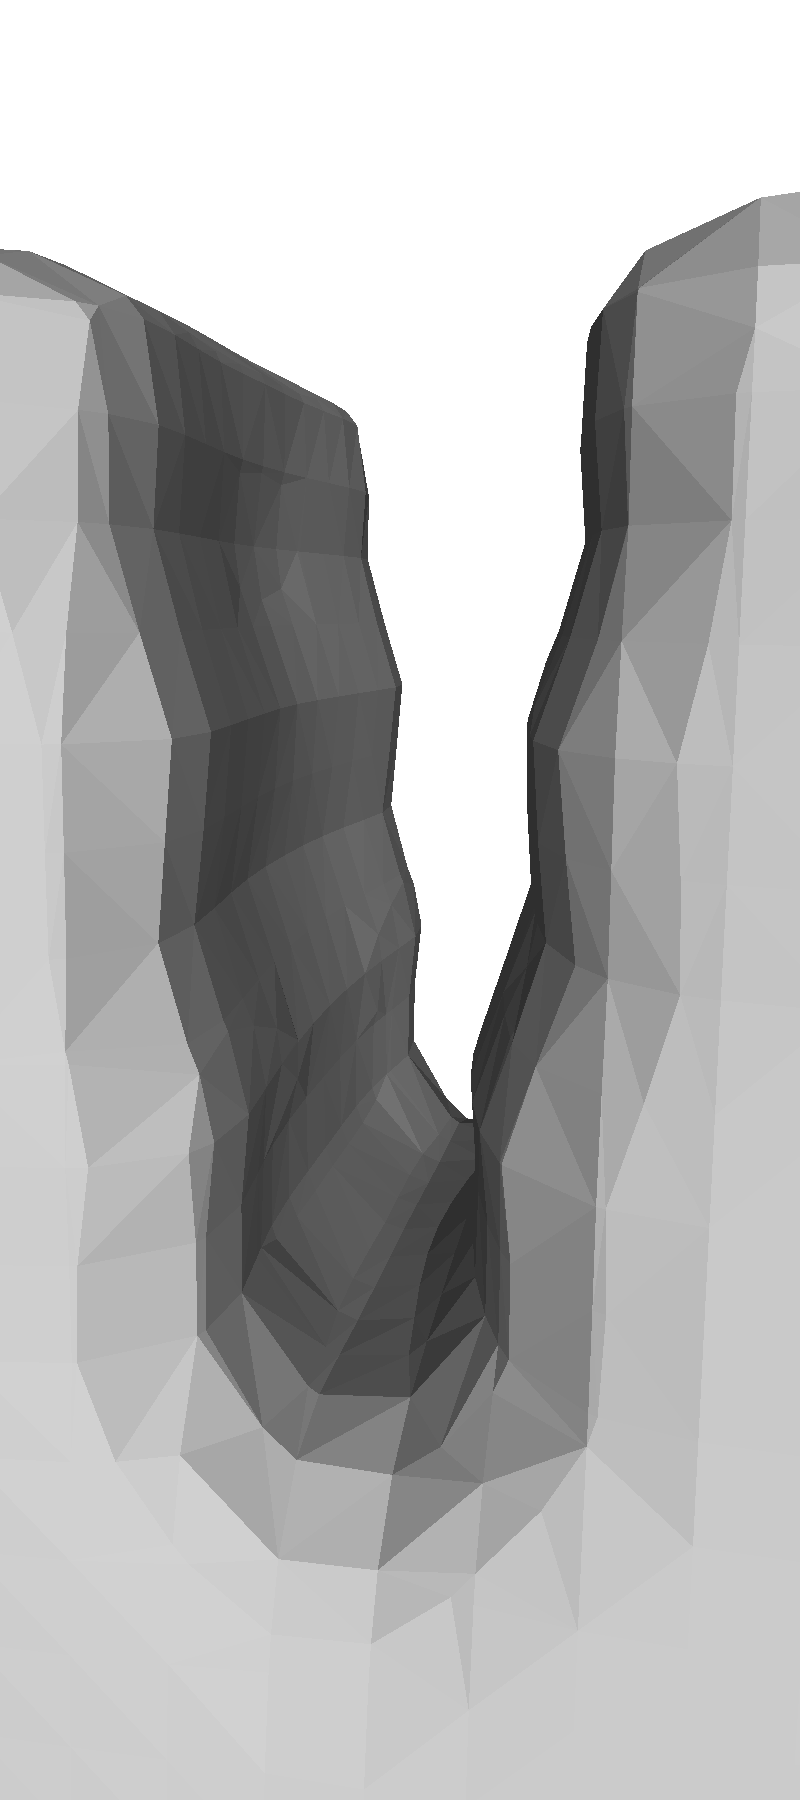
\includegraphics[width=\textwidth]{poi_turbine_groove_100}
		\caption{100}
		\label{fig:poi_turbine_groove_100}
	\end{subfigure}
	\begin{subfigure}[b]{0.24\textwidth}
		\centering
		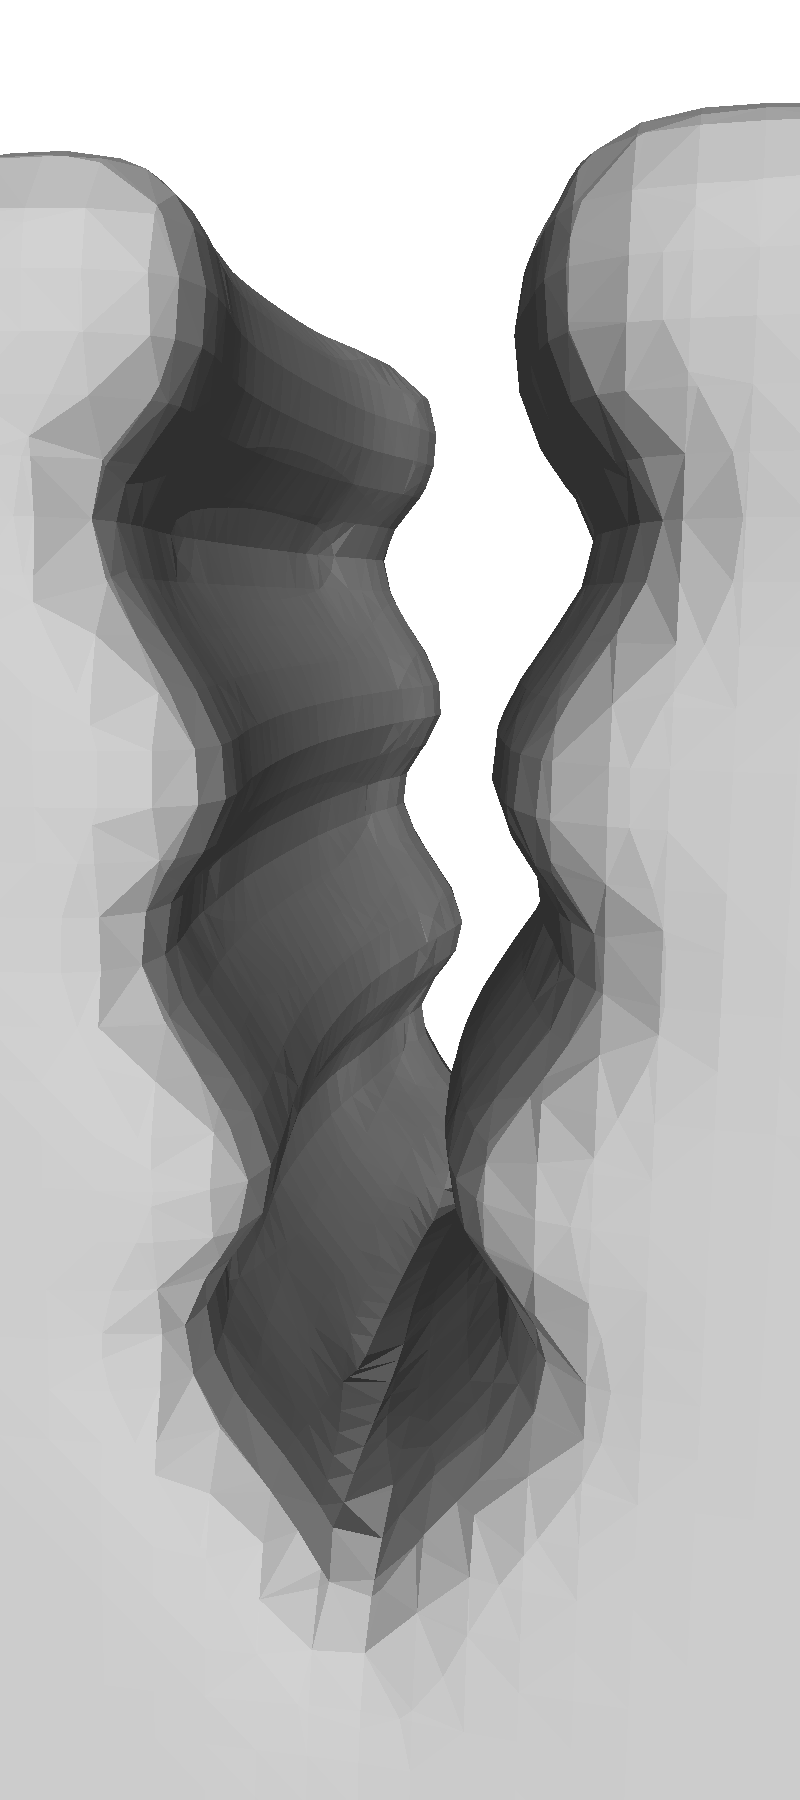
\includegraphics[width=\textwidth]{poi_turbine_groove_200}
		\caption{200}
		\label{fig:poi_turbine_groove_200}
	\end{subfigure}
	\begin{subfigure}[b]{0.24\textwidth}
		\centering
		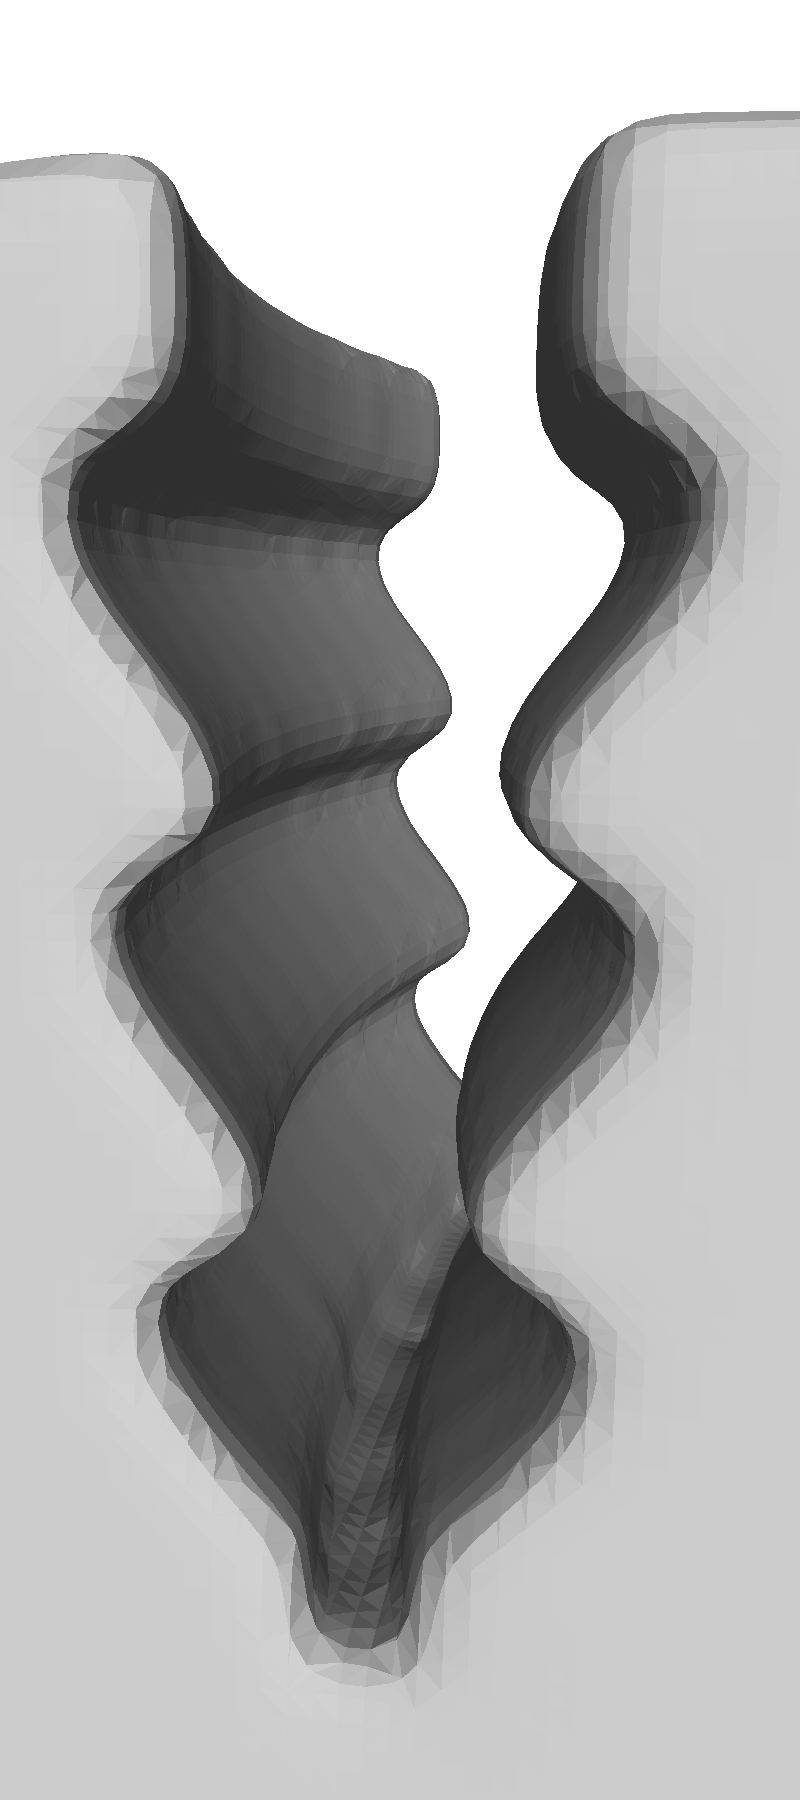
\includegraphics[width=\textwidth]{poi_turbine_groove_400}
		\caption{400}
		\label{fig:poi_turbine_groove_400}
	\end{subfigure}
	\caption{
		Detailed renderings with the same perspective of a groove of the turbine scene using MeshLab.
		The meshes were created using the Poisson surface reconstruction filter of MeshLab run on a point cloud with the resolutions 50, 100, 200 and 400.
	}
	\label{fig:poi_grooves}
\end{figure}
%
At a resolution of 50, the groove is simply sampled too poor for the Poisson reconstruction to create the indentation.
This result is comparable to the BPA's performance at the same resolution in figure \ref{fig:bpa_turbine_groove_50}, where the ball was too big to roll inside the groove.
At a resolution of 100, the groove becomes visible as the indentation is created.
Still, the concave rills inside the notch as well as the indentation at the bottom of the groove are not visible yet.
The rills are acceptably reconstructed at a resolution of 200 while the bottom notch requires a resolution of 400 to appear.
Compared with the tri-dexel approach and similarly to the BPA, the Poisson surface reconstruction also requires roughly twice the resolution of the tri-dexel for a visually comparable output regarding the captured features.
However, as detailed in section \ref{sec:point_cloud_concept}, the main reason for this issue is the richer semantic carried by the tri-dexel image when compared with a point cloud.

Concerning timings, the Poisson surface reconstruction filter of MeshLab is roughly 10 - 20 times slower than the BPA implementation of the VML, \cf table \ref{tbl:bpa_results}.
\Eg, the runtimes for the turbine scene at the resolutions 50, 100, 200 and 400, averaged over 5 runs, are \SI{941}{\milli\second}, \SI{2816}{\milli\second}, \SI{10587}{\milli\second} and \SI{46397}{\milli\second}, respectively, measured using MeshLab.
However, the algorithm employed by MeshLab runs single threaded.
Accounting for this difference, MeshLab's Poisson implementation and the VML's BPA would both require a runtime in the same order of magnitude
During the reconstruction at resolution 400, roughly \SI{400}{\mebi\byte} were allocated, making the Poisson algorithm significantly more light-weight than the BPA.

Similar to the external Poisson surface reconstruction algorithm of MeshLab, any other external algorithm may be run on the point clouds created from the raycaster in section \ref{sec:point_cloud_implementation}.
MeshLab for example further offers an implementation of alpha shapes \cite{alpha_shape}, an own BPA, two marching cubes variants based on MLS \cite{meshlab_mc_mls_1, meshlab_mc_mls_2} as well as an algorithm based on distance fields from the VCG library \cite{vcg}.
Further libraries for point cloud surface reconstruction include the Computational Geometry Algorithms Library (CGAL) \cite{cgal}, the Visualization Toolkit (VTK) \cite{vtk}, QHull \cite{qhull} or the Point Cloud Library (PCL) \cite{pcl}.
